%%
%% This is file `thesis-ex.tex',
%% generated with the docstrip utility.
%%
%% The original source files were:
%%
%% uiucthesis2014.dtx  (with options: `example')
%% 
\def\fileversion{v2.25b} \def\filedate{2017/05/02}
%% Package and Class "uiucthesis2014" for use with LaTeX2e.
\documentclass[12pt,edeposit,fullpage]{uiucthesis2014}

% references at the end of each chapter
\usepackage[round,sectionbib]{natbib}
\usepackage{chapterbib}

\usepackage{amsmath}
\usepackage{amssymb}
\usepackage{bibentry}
\usepackage{graphicx}
\usepackage{hyperref}
\usepackage{caption}
\usepackage{subcaption}
\usepackage{rotating}

\def\aap{{A\&A}}
\def\AaA{{A\&A}}
\def\AJ{{AJ}}
\def\aj{{AJ}}
\def\ApJ{{ApJ}}
\def\apj{{ApJ}}
\def\apjl{{ApJL}}
\def\ApJL{{ApJL}}
\def\ApJSupp{{ApJS}}
\def\MN{{MNRAS}}
\def\mnras{{MNRAS}}
\def\mnrasl{{MNRAS Letters}}
\def\pasp{{PASP}}
\def\jcap{JCAP}
\def\pasj{{PASJ}}
\def\nat{Nature}
\def\ARAA{{ARA\&A}}
\def\apjs{{ApJS}}
\def\araa{{ARA\&A}}
\def\apss{{Ap\&SS}}
\def\cjaa{{ChJAA}}
\def\aaps{{A\&AS}}

\newcommand{\eg}{{e.g., }}
\newcommand{\ie}{{i.e., }}
\newcommand\blfootnote[1]{%
  \begingroup
  \renewcommand\thefootnote{}\footnote{#1}%
  \addtocounter{footnote}{-1}%
  \endgroup
}

% put figure on a new page
\renewcommand{\floatpagefraction}{0.1}

\nocopyrightpage

\begin{document}

\title{Machine Learning Approaches to\\
       Star-galaxy Classification}
\author{Junhyung Kim}
\department{Physics}
\phdthesis
\advisor{Robert J.\ Brunner}
\degreeyear{2018}
\committee{
    Professor Emeritus Jon J.\ Thaler, Chair\\
    Professor Robert J.\ Brunner, Director of Research\\
    Professor George D.\ Gollin\\
    Assistant Professor Alexander G.\ Schwing}
\maketitle

\frontmatter

%% Create an abstract that can also be used for the ProQuest abstract.
%% Note that ProQuest truncates their abstracts at 350 words.
\begin{abstract}
Accurate star-galaxy classification has many important applications in modern precision cosmology.
However, a vast number of faint sources that are detected in the current and
next-generation ground-based surveys may be challenged by poor star-galaxy classification.
Thus, we explore a variety of machine learning approaches to improve
star-galaxy classification in ground-based photometric surveys.
In Chapter~\ref{chapter2}, we present a meta-classification framework that combines existing star-galaxy classifiers,
and demonstrate that our Bayesian combination technique improves the overall performance over any individual classification method.
In Chapter~\ref{chapter3}, we show that a deep learning algorithm called convolutional neural networks
is able to produce accurate and well-calibrated classifications by learning directly from the pixel values of photometric images.
In Chapter~\ref{chapter4}, we study another deep learning technique called generative adversarial networks
in a semi-supervised setting, and demonstrate that our semi-supervised method produces competitive classifications
using only a small amount of labeled examples.

\end{abstract}

%% Create a dedication in italics with no heading, centered vertically
%% on the page.
%\begin{dedication}
%To Father and Mother.
%\end{dedication}

%% Create an Acknowledgements page, many departments require you to
%% include funding support in this.
\chapter*{Acknowledgments}

First and formorest, I would like to thank my advisor, Robert Brunner, for his guidance and support
during my graduate studies at UIUC.
I also wish to thank my committee members, Jon Thaler, George Gollin, and Alex Schwing, for their help and support.
I am also grateful to Matias Carrasco Kind, Yiran Wang, Nacho Sevilla, William Biscarri, Samantha Thrush, Xinyang Lu, and Kelechi Ikegwu.
A special thanks to my father and my wife who endured this long process with me.

\begin{flushright}
--- Edward Junhyung Kim
\end{flushright}

\vspace{10mm}

This work was supported in part by the National Science Foundation Grant
No.\ AST-1313415.
This work used the Extreme Science and Engineering Discovery Environment
(XSEDE), which is supported by National Science Foundation grant number
ACI-1053575.
This work is based on observations obtained with MegaPrime/MegaCam, a
joint project of CFHT and CEA/DAPNIA, at the Canada-France-Hawaii
Telescope (CFHT) which is operated by the National Research Council
(NRC) of Canada, the Institut National des Sciences de l'Univers of
the Centre National de la Recherche Scientifique (CNRS) of France, and
the University of Hawaii. This research used the facilities of the
Canadian Astronomy Data Centre operated by the National Research
Council of Canada with the support of the Canadian Space Agency.
CFHTLenS data processing was made possible thanks to significant
computing support from the NSERC Research Tools and Instruments grant
program.
Funding for the DEEP2 survey has been provided by NSF grants AST-0071048,
AST-0071198, AST-0507428, and AST-0507483. 
Funding for SDSS-III has been provided by the Alfred P. Sloan Foundation, the
Participating Institutions, the National Science Foundation, and the U.S.
Department of Energy Office of Science. The SDSS-III web site is
http://www.sdss3.org/.
This work used data from the 
VIMOS Public Extragalactic Redshift Survey (VIPERS).
VIPERS has been performed using the ESO Very Large Telescope, under the "Large
Programme" 182.A-0886. The participating institutions and funding agencies are
listed at http://vipers.inaf.it/.
This work used data from the VIMOS VLT Deep Survey, obtained from the VVDS
database operated by Cesam, Laboratoire d'Astrophysique de Marseille, France.

%% The thesis format requires the Table of Contents to come
%% before any other major sections, all of these sections after
%% the Table of Contents must be listed therein (i.e., use \chapter,
%% not \chapter*).  Common sections to have between the Table of
%% Contents and the main text are:
%%
%% List of Tables
%% List of Figures
%% List Symbols and/or Abbreviations
%% etc.

\tableofcontents
%\listoftables
%\listoffigures

%% Create a List of Abbreviations. The left column
%% is 1 inch wide and left-justified
%\chapter{List of Abbreviations}
%
%\begin{symbollist*}
%\item[CA] Caffeine Addict.
%\item[CD] Coffee Drinker.
%\end{symbollist*}

%% Create a List of Symbols. The left column
%% is 0.7 inch wide and centered
%\chapter{List of Symbols}
%
%\begin{symbollist}[0.7in]
%\item[$\tau$] Time taken to drink one cup of coffee.
%\item[$\mu$g] Micrograms (of caffeine, generally).
%\end{symbollist}

\mainmatter

\chapter{Introduction}


\section{Star-galaxy Classification in Photometric Surveys}


Currently ongoing and upcoming large-scale surveys, such as the Dark Energy Survey (DES)
and the Large Synoptic Survey Telescope (LSST), are purely photometric surveys,
where digital images of the sky are obtained and subsequently analyzed.
To quantify the brightness of a source in a photometric image,
we count the number of photons from the source within a fixed aperture
(\eg a circle or a two-dimensional Gaussian).
This brightness measurement is expressed in units of magnitude ---
a logarithmic unit in which the fainter a source appears the larger its magnitude.
In mathematical terms, the apparent magnitude $m$ in a spectral band $\lambda$ is given by
\begin{equation}
m_{\lambda} = - 2.5 \log_{10} \frac{ F_{\lambda} }{ F_{\lambda,0} },
\end{equation}
where $F_{\lambda}$ is the observed flux using the photometric filter $\lambda$ ,
and $F_{\lambda,0}$ is the reference flux (\ie zero-point) for that filter.
Photometric surveys use filters on telescopes to allow only light around
a specific wavelength to pass.
Figure~\ref{fig:filters} shows the wavelengths of the five filters (named $u$, $g$, $r$, $i$, $z$)
of the Sloan Digital Sky Survey (SDSS).
Before these photometric data can be used for a scientific analysis, however, they must be classified,
which for most sources is either a star or a galaxy.

Stars are in our Milky Way galaxy and are close to us compared to distant galaxies.
Due to their small physical size, however, almost all stars appear as compact point sources
in photometric images.
Galaxies, despite being farther away, generally subtend a larger angle, and thus
appear as extended sources.
However, as Figure~\ref{fig:sg_mag} demonstrates, it becomes increasingly difficult
to separate stars from galaxies due to a large number of unresolved galaxies at faint magnitudes.
Since the number of galaxies grows exponentially with magnitude, 
this implies that the majority of sources that are detected in the current and
next-generation ground-based surveys may be challenged by poor star-galaxy classification.
Furthermore, due to the sheer number of stars and galaxies,
this classification has to be automated.
For example, the SDSS has obtained photometric observations of more than $3 \times 10^8$ objects
\citep{eisenstein2011sdss},
and the LSST will produce a catalog of $2 \times 10^{10}$ galaxies and a similar number of stars
\citep{ivezic2008lsst}.
Thus, there is a need for a robust, automated classification technique for large ground-based photometric surveys.

The classification of stars vs.\ galaxies has many important applications in precision cosmology.
As a basic example, in a homogeneous universe with a Euclidean geometry for three-dimensional space,
the number counts of galaxies as a function of magnitude follows
\begin{equation}
N \left( m_{\lambda} \right) \propto 10^{ 0.6 \left( m_{\lambda} - m_{\lambda,0} \right) }.
\end{equation}
By comparing this relation with the predictions of a Friedmann-Robertson-Walker (FRW) universe
(\ie the standard model of cosmology),
\citet{yasuda2001galaxy} show that our universe does not have a Euclidean geometry for
three-dimensional space.
Without a reliable method for separating stars from unresolved galaxies, 
we risk underestimating the number density of galaxies by rejecting all unresolved galaxies,
while including them could result in significant contamination of the galaxy sample.
Furthermore, the accurate separation of stars and galaxies in faint samples
significantly improves our ability to
(i) measure auto-correlation functions of luminous galaxies \citep{ross2011ameliorating},
(ii) control the systematic errors in the weak lensing shear measurement \citep{soumagnac2015star},
(iii) map the signature of baryon acoustic oscillations \citep{anderson2014clustering}, and
(iv) identify electromagnetic counterparts to gravitational wave sources \citep{miller2017preparing},
among other things.

Given the importance of this classification problem, it is not surprising that a variety of
different strategies have been developed.
The most commonly used method to classify stars and galaxies in large sky surveys is the morphological separation
\citep{sebok1979optimal, kron1980photometry, valdes1982resolution, yee1991faint, vasconcellos2011decision,
henrion2011bayesian}.
It relies on the assumption that stars appear as point sources while galaxies appear as resolved sources.
For example, a popular technique in the weak lensing community \citep{Kaiser1995}
makes a hard cut in the space of photometric attributes as shown in Figure \ref{fig:intro_morc}.
As the Figure shows, there is a distinct locus
produced by point sources in the half-light radius vs.\ the $i$-band magnitude plane.
(The half-light radius is the effective radius at which half of the total light of an object is contained.)
A rectangular cut in this size-magnitude plane separates point sources
(which are presumed to be stars) from resolved sources (which are presumed to be galaxies).

However, such a hard cut in a low-dimensional parameter space has disadvantages:
it does not break down gracefully; its treatment of measurement uncertainties is too simplistic;
it uses a rather limited subset of the full information available;
and it ignores a priori information like the expected demographics of the source populations.
Furthermore, currently ongoing and upcoming large photometric surveys
will detect a vast number of unresolved galaxies at faint magnitudes.
Near a survey's limit, the photometric observations cannot reliably separate stars from unresolved galaxies
by morphology alone without leading to incompleteness and contamination in the star and galaxy samples.

\section{Machine Learning}

\subsection{Supervised Learning}

The systematic misclassification of sources can be mitigated by using machine learning algorithms.
Machine learning methods have the advantage that it is easier to include extra information,
such as shape information or different model magnitudes.
Machine learning techniques are usually categorized into two main types: supervised and unsupervised learning approaches.
In the supervised learning approach, the input attributes (\ie the values that describe the properties of each objects \eg magnitudes),
$\mathbf{X}= \{ \mathbf{x}_1,\mathbf{x}_2,\dots,\mathbf{x}_N \}$,
are provided along with the desired output values (\eg star or galaxy),
$\mathbf{y} = \{ y_1, y_2, \dots, y_N \}$, in a labeled set of input-output pairs
$\mathbf{D} = \{ \left( \mathbf{x}_i, y_i \right) \}_{i = 1}^N$.
Here, $\mathbf{D}$ is the training set, and $N$ is the number of training examples.
The goal of supervised learning is then to estimate a function that maps $f: \mathbf{X} \rightarrow \mathbf{y}$.
As we discuss in the following chapters, it is desirable for the algorithm to return a probability.
To emphasize the need for probabilistic predictions, we formulate the goal of supervised learning as folows:
a probabilistic supervised learning algorithm infers the probability distribution $P( \mathbf{y} | \mathbf{X}, \mathbf{D} )$
over possible labels, given the input $\mathbf{X}$ and training set $\mathbf{D}$.
We use the conditioning bar $|$ to explicitly show that the probability is conditional on both
the input $\mathbf{X}$ and the training set $\mathbf{D}$.
When we have a set of multiple models to choose from, we explicitly condition the probability on the set of models and write
$P \left( \mathbf{y} | \mathbf{X}, \mathbf{D}, \mathbf{M} \right)$, where $\mathbf{M}$ is the set of models.
However, if it is clear from the context which model we use to make predictions, we drop $\mathbf{M}$ although
it is implied that the probability is conditional on the form of model.

To obtain the truth labels for the training data,
we use spectroscopy to measure the spectrum of electromagnetic radiation
from stars and galaxies.
Although modern spectrometers are more complex,
a spectrometer, in its most basic form, consists of a slit,
a prism or diffraction grating (to split the light into its component colors), and a detector.
We can use spectroscopy to measure many properties of distant stars and galaxies,
such as their chemical composition, temperature, and distance, and thus
spectral classification can be used as the ground truth for classifying sources in photometric images.

\subsection{Neural Networks}

As an example of a supervised learning algorithm, we provide a brief description of
\textit{artificial neural networks} (ANN)---the most widely used machine learning algorithm in astronomy.
The use of neural networks in astronomy goes as far back as the mid 1980s \citep{jeffrey1986optimization}.
ANN was first applied to the star-galaxy classification problem by \citet{odewahn1992automated},
and it has become a core part of the popular astronomical image processing software \textsc{SExtractor}~\citep{bertin1996sextractor}.

The original motivation for ANNs was to simulate neurons in the human brain.
A neuron in the human brain receives signals from other neurons through synaptic connections.
If the combination of these signals exceeds a certain threshold,
the neuron will fire and send a signal to other neurons.
Intelligence is believed to be the collective effect of
approximately $10^{11}$ neurons firing.
An artificial neuron in most artificial neural networks is represented
as a mathematical function that models a biological neural structure
(Figure~\ref{fig:intro_neuron_a}).
Let $\mathbf{x}=\left(x_1,x_2,\dots,x_n\right)$ be a vector of inputs to a given neuron,
$\mathbf{w}=\left(w_1,w_2,\dots,w_n\right)$ be a vector of weights, and
$b$ be the bias.
Then, the output of the neuron is
\begin{equation}
  y = \sigma \left( \mathbf{w} \cdot \mathbf{x} + b \right),
  \label{eq:intro_neuron_output}
\end{equation}
where $\sigma$ is the activation function (or \textit{non-linearity}).
Common activation functions include the sigmoid function,
\begin{equation}
\sigma(x)=1/\left(1+e^{-x}\right),
\end{equation}
the hyperbolic tangent function,
\begin{equation}
\sigma(x)=\tanh(x),
\end{equation}
and the rectified linear unit \citep[ReLU;][]{nair2010rectified},
\begin{equation}
\sigma(x)=\max(0, x).
\end{equation}
Typical neurons are organized as layers, where each neuron in one layer is connected to the neurons of the subsequent layer.
A schematic representation is shown in Figure~\ref{fig:intro_neuron_b}.
All layers except the input and output layers are conveniently called hidden layers.

The training uses an algorithm to a set of weights and biases such that, given $N$ samples, the output from the network
$\mathbf{y}=\left(\hat{y}_1, \hat{y}_2, \dots, \hat{y}_N \right)$
approximates the desired output
$\mathbf{y} = \left(y_1, y_2, \dots, y_N \right)$
as closely as possible for all input
$\mathbf{X}=\left(\mathbf{x}_1,\mathbf{x}_2,\dots,\mathbf{x}_N\right)$.
We can formulate this as the minimization of a loss function $L(\mathbf{y},\hat{\mathbf{y}})$ over the training data.
A common form of the loss function is the \textit{cross-entropy},
\begin{equation}
  L(y_j, \hat{y}_j) = - \frac{1}{N} \sum_{j=1}^{N} y_j  \log_2 \hat{y}_j
    + (1 - y_j)  \log_2 (1 - \hat{y}_j).
  \label{eq:intro_cross_entropy}
\end{equation}
where $y_j$ is the actual truth value (\eg 0 or 1) of the $j$-th data, and
$\hat{y}_j$ is the probability prediction made by the model.

To find the weights $\mathbf{w}$ and biases $\mathbf{b}$ which minimize the loss,
we use a technique called \textit{gradient descent},
where we use the following rules to update the parameters in each layer $l$:
\begin{align}
  \mathbf{w}_l &\rightarrow
  \mathbf{w}_l^{\prime}
  = \mathbf{w}_l - \eta \frac{\partial L}{\partial \mathbf{w}_l} \nonumber \\
  \mathbf{b}_l &\rightarrow
  \mathbf{b}_l^{\prime}
  = \mathbf{b}_l - \eta \frac{\partial L}{\partial \mathbf{b}_l},
  \label{eq:intro_gradient_descent}
\end{align}
where $\eta$ is a small, positive number known as the \textit{learning rate}.
The gradients in \ref{eq:intro_gradient_descent} can be computed using the
\textit{backpropagation} procedure~\citep{rumelhart1988learning},
which is nothing more than an application of the chain rule for derivatives.

\subsection{Unsupervised and Semi-supervised Learning}

In contrast to supervised learning, in which the truth labels are provided,
unsupervised learning does not utilize the desired output during the learning process.
Instead, we are only given unlabeled inputs $\mathbf{D}= \{ \mathbf{x}_i \}_{i=1}^N$,
and the data is clustered into different classes or categories.
In other words, unsupervised learning attempts to infer the probability distribution of the form $P(\mathbf{x}_i)$.
Unsupervised machine learning techniques are less common, in part due to the successes of purely supervised learning.
Semi-supervised learning falls between supervised learning, where training data are completely labeled,
and unsupervised learning, where all training data are unlabeled.
Semi-supervised techniques make use of a large amount of unlabeled data, in conjunction with a small amount of labeled data,
to better capture the underlying data distribution.
We expect unsupervised and semi-supervised learning to become more important, since
it is unclear if sufficient training data will be available in future ground-based photometric surveys and
there will be many orders of magnitude more unlabeled than labeled data available in future ground-based imaging surveys.

\section{Thesis Structure}

In the following chapters, we explore a variety of statistical and machine learning approaches to push the limits of
star-galaxy classification in ground-based photometric surveys.
Each chapter is self-contained and has its own references.

In Chapter~\ref{chapter2}, we present a novel meta-classification
framework that combines and fully exploits different techniques
to produce a more robust star-galaxy classification.
To demonstrate this hybrid, ensemble approach,
we combine a purely morphological classifier,
a supervised machine learning method based on random forest,
an unsupervised machine learning method based on self-organizing maps,
and a hierarchical Bayesian template fitting method.
Using data from the Canada-France-Hawaii Telescope Lensing Survey (CFHTLenS),
we consider different scenarios:
when a high-quality training set is available with spectroscopic labels,
and when the demographics of sources in a low-quality training set
do not match the demographics of objects in the test data set.
We demonstrate that our Bayesian combination technique improves
the overall performance over any individual classification method
in these scenarios.

In Chapter~\ref{chapter3}, we present a star-galaxy classification framework that uses a supervised machine learning algorithm called
convolutional neural networks (ConvNets).
Most existing star-galaxy classifiers use the reduced summary information from catalogs,
requiring careful feature extraction and selection.
Deep ConvNets allow a machine to automatically learn the features directly from images,
minimizing the need for input from human experts.
Using data from the SDSS and CFHTLenS,
we demonstrate that ConvNets are able to produce accurate and well-calibrated probabilistic classifications that are competitive with
conventional machine learning techniques.

In Chapter~\ref{chapter4}, we study the application of a deep learning technique called generative adversarial networks (GANs)
to the star-galaxy classification problem in a semi-supervised setting.
As current and forthcoming photometric surveys probe large cosmological volumes,
the majority of photometric observations are too faint for a uniform spectroscopic follow-up.
As a result, the number of unlabeled data available for training machine learning algorithms will be orders of magnitude
greater than the number of labeled data.
Semi-supervised learning techniques are of great interest since they are able to capture the underlying data distribution
with only a small amount of labeled data.
Using photometric images from the SDSS, we demonstrate that semi-supervised GANs are able to produce
accurate and well-calibrated classifications using only a small amount of labeled examples.
We also show that the number count distributions of the images generated by GAN follow a similar distribution to
the SDSS photometric sample.

In Chapter \ref{chapter5}, we outline our conclusions.

\newpage
\section{Figures and Tables}

\vspace{100pt}

\begin{figure}[htp]
  \centering
  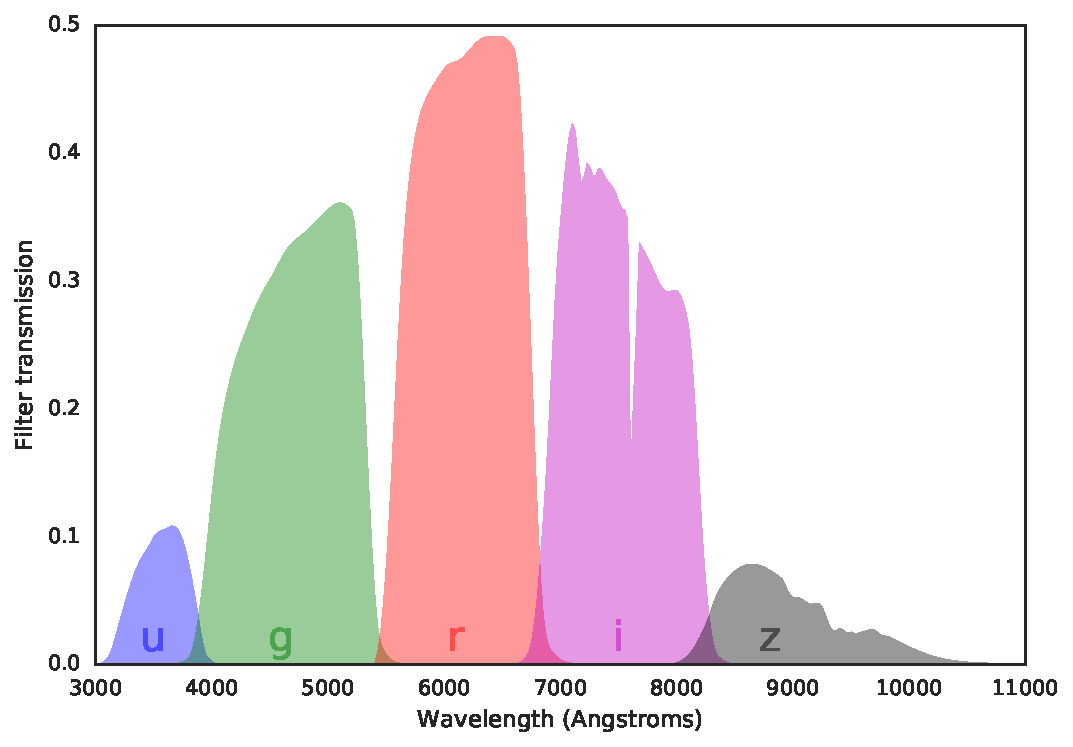
\includegraphics[width=0.8\textwidth]{figures/filters.pdf}
  \caption{The SDSS $ugriz$ filter transmission curves.}
  \label{fig:filters}
\end{figure}

\begin{sidewaysfigure}[htp]
  \centering
  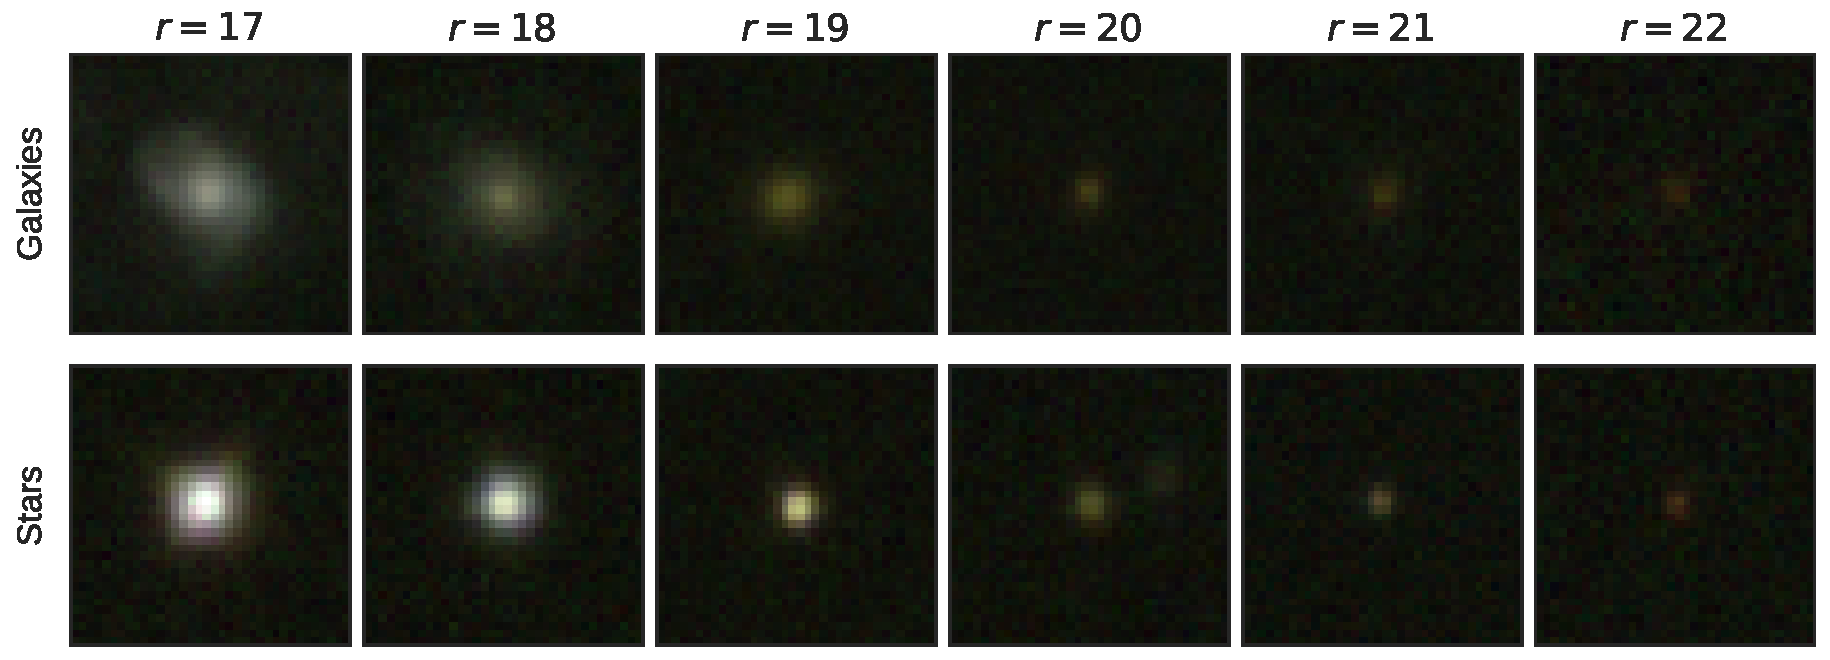
\includegraphics[width=\textwidth]{figures/sgstamps.pdf}
  \caption{Sample images of stars (top row) and galaxies (bottom row) from the SDSS survey
  at different magnitudes ($r$-band).
  Note that it becomes increasingly difficult to classify sources at fainter magnitudes,
  where we have the majority of the detected sources.}
  \label{fig:sg_mag}
\end{sidewaysfigure}

\begin{figure}[htp]
  \centering
  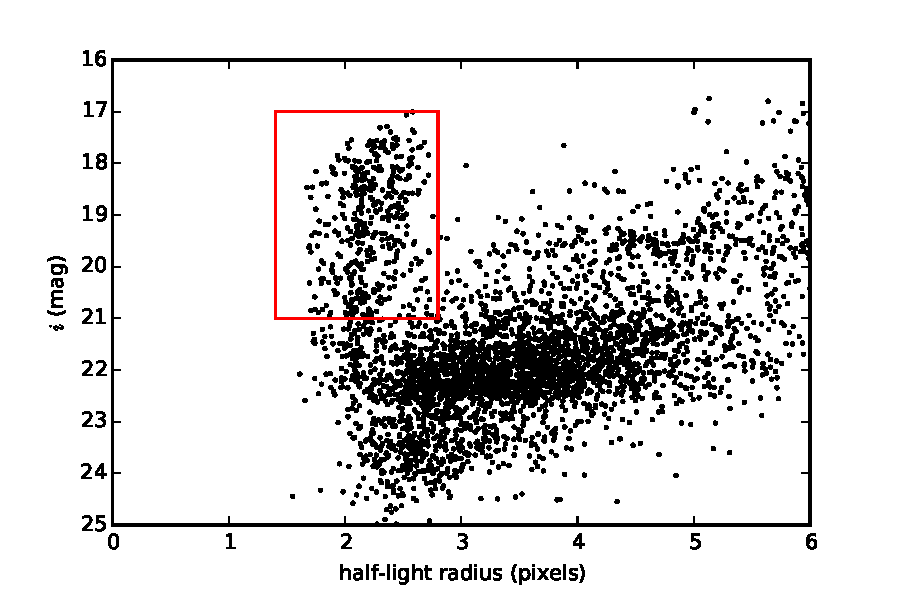
\includegraphics{figures/morph.pdf}
  \caption{Half-light radius vs.\ magnitude.}
  \label{fig:intro_morc}
\end{figure}

\begin{sidewaysfigure}
  \centering
  \begin{subfigure}[]{0.49\linewidth}
    \centering
    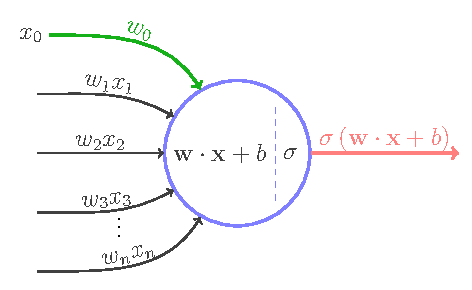
\includegraphics[width=0.6\textwidth]{figures/neuron.pdf}
    \caption{}
    \label{fig:intro_neuron_a}
  \end{subfigure}
  \begin{subfigure}[]{0.49\linewidth}
    \centering
    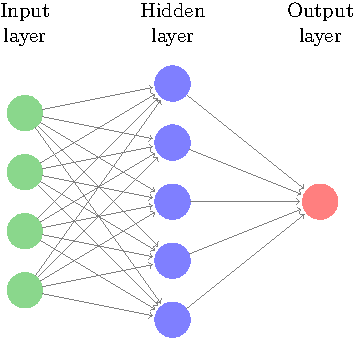
\includegraphics[width=0.6\textwidth]{figures/network.pdf}
    \caption{}
    \label{fig:intro_neuron_b}
  \end{subfigure}
  \caption{
    (a) A mathematical model of a biological neuron.
    (b) A schematic diagram of a neural network with one hidden layer.
    }
\end{sidewaysfigure}


\clearpage
\bibliographystyle{plainnat}
\bibliography{thesisbib}
\chapter{A Hybrid Ensemble Learning Approach to Star-galaxy Classification}
  \label{chapter2}

\blfootnote{
This chapter contains material from the following previously published article:
\nobibliography{thesisbib}
\begin{itemize}
\item\bibentry{kim2015hybrid}
\end{itemize}
}
\section{Introduction}
  \label{section:introduction}

The problem of source classification is fundamental to astronomy
and goes as far back as \citet{messier1781catalogue}.
A variety of different strategies have been developed 
to tackle this long-standing problem,
and yet there is no consensus on
the optimal star-galaxy classification strategy.
The most commonly used method to classify stars and galaxies
in large sky surveys is the morphological separation
~\citep{sebok1979optimal, kron1980photometry, valdes1982resolution,
yee1991faint, vasconcellos2011decision,
henrion2011bayesian}.
It relies on the assumption that
stars appear as point sources
while galaxies appear as resolved sources.
However,
currently ongoing and upcoming large photometric surveys,
such as the Dark Energy Survey (DES) and the Large Synoptic Survey Telescope (LSST),
will detect a vast number of unresolved galaxies at faint magnitudes.
Near a survey's limit, the photometric observations
cannot reliably separate stars from unresolved galaxies
by morphology alone without leading to
incompleteness and contamination in the star and galaxy samples.

The contamination of unresolved galaxies can be mitigated
by using training based algorithms.
Machine learning methods have the advantage that
it is easier to include extra information,
such as concentration indices, shape information,
or different model magnitudes.
However,
they are only reliable within the limits of the training data,
and it can be difficult to extrapolate these algorithms
outside the parameter range of the training data.
These techniques can be further categorized into
supervised and unsupervised learning approaches.

In supervised learning, 
the input attributes (\eg magnitudes or colors)
are provided along with the truth labels (\eg star or galaxy).
\citet{odewahn1992automated} pioneered
the application of neural networks
to the star-galaxy classification problem,
and it has become a core part of
the astronomical image processing software
\textsc{SExtractor}~\citep{bertin1996sextractor}.
Other successfully implemented examples include
decision trees~\citep{weir1995automated, suchkov2005census, ball2006robust,
sevilla2015effect}
and Support Vector Machines~\citep*{Fadely2012}.
Unsupervised machine learning techniques
are less common,
as they do not utilize the truth labels during the training process,
and only the input attributes are used.

Physically based template fitting methods
have also been used for the star-galaxy classification
problem~\citep{robin2007stellar, Fadely2012}.
Template fitting approaches infer a source's properties
by finding the best match between
the measured set of magnitudes (or colors)
and the synthetic set of magnitudes (or colors)
computed from a set of spectral templates.
Although it is not necessary to obtain
a high-quality spectroscopic training sample,
these techniques do require
a representative sample of theoretical or empirical templates
that span the possible spectral energy distributions (SEDs)
of stars and galaxies.
Furthermore, they are not exempt from uncertainties
due to measurement errors on the filter response curves,
or from mismatches between the observed magnitudes
and the template SEDs.

In this chapter,
we present a novel star-galaxy classification framework
that combines and fully exploits different classification techniques
to produce a more robust classification.
In particular,
we show that the combination of a morphological separation method,
a template fitting technique, a supervised machine learning method,
and an unsupervised machine learning algorithm
can improve the overall performance over any individual method.
In Section~\ref{section:classification_methods},
we describe each of the star-galaxy classification methods.
In Section~\ref{section:classification_combination_methods},
we describe different classification combination techniques.
In Section~\ref{section:data},
we describe the Canada-France Hawaii Telescope Lensing Survey (CFHTLenS)
data set with which we test the algorithms.
In Section~\ref{section:results_and_discussion},
we compare the performance of our combination techniques
to the performance of the individual classification techniques.
Finally, we outline our conclusions in Section~\ref{section:conclusions}.

\section{Classification Methods}
  \label{section:classification_methods}

In this section, we present
four distinct star-galaxy classification techniques.
The first method is a morphological separation method,
which uses a hard cut in the half-light radius vs.\ magnitude plane.
The second method is
a supervised machine learning technique named TPC
(Trees for Probabilistic Classification),
which uses prediction trees and a random forest~\citep{carrascokind2013tpz}.
The third method is
an unsupervised machine learning technique named SOMc,
which uses self-organizing maps (SOMs) and a random atlas
to provide a classification~\citep{carrascokind2014somz}.
The fourth method is
a Hierarchical Bayesian (HB) template fitting technique
based on the work by \citet{Fadely2012},
which fits SED templates from star and galaxy libraries
to an observed set of measured flux values.

Collectively, these four methods represent the majority of all
standard star-galaxy classification approaches published in the literature.
It is very likely that any new classification technique would be
functionally similar to one of these four methods.
Therefore, any of these four methods could in principle be replaced by a similar method. 


\subsection{Morphological Separation}

The simplest and perhaps the most widely used approach
to star-galaxy classification is
to make a hard cut in the space of photometric attributes.
As a first-order morphological selection of point sources,
we adopt a technique that is popular among the weak lensing 
community~\citep*{Kaiser1995}.
As Figure~\ref{fig:morph} shows, there is a distinct locus
produced by point sources in the half-light radius
(estimated by \textsc{SExtractor}'s FLUX\_RADIUS parameter)
vs.\ the $i$-band magnitude plane.
A rectangular cut in this size-magnitude plane separates point sources,
which are presumed to be stars,
from resolved sources,
which are presumed to be galaxies.
The boundaries of the selection box are determined by
manually inspecting the size-magnitude diagram.



One of the disadvantages of such cut-based methods is
that it classifies every source with absolute certainty.
It is difficult to justify such a decisive classification
near a survey's magnitude limits,
where measurement uncertainties generally increase.
A more informative approach is to provide probabilistic classifications.
Although a recent work by \citet{henrion2011bayesian}
implemented a probabilistic classification using a Bayesian approach
on the morphological measurements alone,
here we use a cut-based morphological separation
to demonstrate the advantages of our combination techniques.
In particular, we later show that
the binary outputs (\ie 0 or 1) of cut-based methods
can be transformed into
probability estimates by combining them
with the probability outputs from other
probabilistic classification techniques,
such as TPC, SOMc, and HB.


\subsection{Supervised Machine Learning: TPC}
  \label{sec:tpc}

TPC is a parallel, supervised machine learning algorithm
that uses prediction trees and random forest 
techniques~\citep{breiman1984classification, breiman2001random}
to produce a star-galaxy classification.
TPC is a part of a publicly available software package called \textsc{MLZ} (Machine Learning for Photo-$z$).
The full software package includes:
\textsc{TPZ}, a supervised photometric redshift (photo-$z$)
estimation technique
\citep[regression mode;][]{carrascokind2013tpz};
TPC, a supervised star-galaxy classification technique
(classification mode);
\textsc{SOM}$z$, an unsupervised photo-$z$ technique
\citep[regression mode;][]{carrascokind2014somz};
and
SOMc, an unsupervised star-galaxy classification technique
(classification mode).

TPC uses classification trees,
a type of prediction trees that are designed to
provide a classification or predict a discrete category.
Prediction trees are built by asking a sequence of questions
that recursively split the data into branches
until a terminal leaf is created
that meets a stopping criterion
(\eg a minimum leaf size).
The optimal split dimension is decided by
choosing the attribute that maximizes
the \textit{Information Gain} ($I_G$), which is defined as

\begin{equation} \label{eq:information_gain}
  I_G \left(D_{\mathrm{node}}, X\right)
  = I_d \left( D_{\mathrm{node}} \right)
  - \sum_{x \in \mathrm{values}(X)}
  \frac{|D_{\mathrm{node}, x}|}{|D_{\mathrm{node}}|}
  I_d \left( D_{\mathrm{node}, x} \right),
\end{equation}

\noindent
where $D_{\mathrm{node}}$ is the training data in a given node,
$X$ is one of the possible dimensions (\eg magnitudes or colors)
along which the node is split, and
$x$ are the possible values of a specific dimension $X$.
$|D_{\mathrm{node}}|$ and $|D_{\mathrm{node}, x}|$ are the size of the total training data
and the number of objects in a given subset $x$ within the current node,
respectively.
$I_d$ is the impurity degree index,
and TPC can calculate $I_d$
from any of the three standard different impurity indices:
\textit{information entropy}, \textit{Gini impurity},
and \textit{classification error}.
In this work, we use the information entropy,
which is defined similarly to the thermodynamic entropy:

\begin{equation}
  I_d \left( D \right)
  = - f_g \log_{2} f_g - \left(1 - f_g\right) \log_{2} \left(1 - f_g\right),
\end{equation}

\noindent
where $f_g$ is the fraction of galaxies in the training data.
At each node in our tree,
we scan all dimensions to identify the split point that
maximizes the information gain as defined by Equation~\ref{eq:information_gain},
and select the attribute that maximizes the impurity index overall.

In a technique called random forest,
we create bootstrap samples
(\ie $N$ randomly selected objects with replacement)
from the input training data
by sampling repeatedly from the magnitudes and colors
using their measurement errors.
We use these bootstrap samples to construct
multiple, uncorrelated prediction trees
whose individual predictions are aggregated to produce
a star-galaxy classification for each source.

We also use a cross-validation technique called
Out-of-Bag~\citep[OOB;][]{breiman1984classification, carrascokind2013tpz}.
When a tree (or a map) is built in TPC (or SOMc),
a fraction of the training data, usually one-third,
is left out and not used in training the trees (or maps).
After a tree is constructed using two-thirds of the training data,
the final tree is applied to the remaining one-third
to make a classification.
This process is repeated for every tree,
and the predictions from each tree are aggregated
for each object to make the final star-galaxy classification.
We emphasize that if an object is used for training a given tree,
it is never used for subsequent prediction by that tree.
Thus, the OOB data is an unbiased estimation of the errors
and can be used as cross-validation data
as long as the OOB data remain similar to the final test data set.
The OOB technique can also provide extra information such as
a ranking of the relative importance of the input attributes
used in the prediction.
The OOB technique can prove extremely valuable
when calibrating the algorithm,
when deciding which attributes to incorporate in the construction of the trees,
and when combining this approach with other techniques.


\subsection{Unsupervised Machine Learning: SOMc}

A self-organizing map~\citep{kohonen1990self, kohonen2001self}
is an unsupervised, artificial neural network algorithm
that is capable of projecting high-dimensional input data
onto a low-dimensional map
through a process of competitive learning.
In astronomical applications,
the high-dimensional input data can be
magnitudes, colors, or some other photometric attributes.
The output map is usually chosen to be two-dimensional
so that the resulting map can be used for visualizing
various properties of the input data.
The differences between a SOM and
typical neural network algorithms are
that a SOM is unsupervised,
there are no hidden layers and therefore no extra parameters,
and it produces a direct mapping
between the training set and the output network.
In fact, a SOM can be viewed as a non-linear generalization
of a principal component analysis (PCA) algorithm~\citep{yin2008self}.

The key characteristic of SOM is that
it retains the topology of the input training set,
revealing correlations between input data that are not obvious.
The method is unsupervised:
the user is not required to specify the desired output
during the creation of the lower-dimensional map,
and the mapping of the components from the input vectors
is a natural outcome of the competitive learning process.

During the construction of a SOM,
each node on the two-dimensional map is represented by
weight vectors of the same dimension
as the number of attributes used to create the map itself.
In an iterative process,
each object in the input sample is individually used
to correct these weight vectors.
This correction is determined so that the specific neuron (or node),
which at a given moment best represents the input source,
is modified along with the weight vectors
of that node's neighboring neurons.
As a result, this sector within the map
becomes a better representation of the current input object.
This process is repeated for every object in the training data,
and the entire process is repeated for several iterations.
Eventually, the SOM converges to its final form where
the training data is separated into groups of similar features.
Although the spectroscopic labels are not used at all
in the learning process, they are used
(only after the map has been constructed)
to generate predictions for each cell in the resulting two-dimensional map.

In a similar approach to random forest in TPZ and TPC,
SOM$z$ uses a technique called \textit{random atlas}
to provide photo-$z$ estimation \citep{carrascokind2014somz}.
In random atlas, the prediction trees of random forest are replaced by maps,
and each map is constructed from different bootstrap samples
of the training data.
Furthermore, we create random realizations of the training data
by perturbing the magnitudes and colors by their measurement errors.
For each map, we can either use all available attributes,
or randomly select a subsample of the attribute space.
This SOM implementation can also be
applied to the classification problem,
and we refer to it as SOMc
in order to differentiate it from 
the photo-$z$ estimation problem (regression mode).
We also use the random atlas approach
in some of the classification combination approaches as discussed in
Section~\ref{section:classification_combination_methods}.

One of the most important parameter in SOMc
is the topology of the two-dimensional SOM,
which can be rectangular, hexagonal, or spherical.
In our SOM implementation, it is also possible
to use periodic boundary conditions for the non-spherical cases.
The spherical topology is by definition periodic and
is constructed by using
\textsc{HEALPIX}~\citep{gorski2005healpix}.
Similar to TPC,
we use the OOB technique to make an unbiased estimation of errors.
We determine the optimal parameters by performing
a grid search in the parameter space of different toplogies,
as well as other SOM parameters, for the OOB data.
We find that the spherical topology gives the best performance
for the CFHTLenS data, likely due to its natural periodicity.
Thus, we use a spherical topology to classify stars and galaxies
in the CFHTLenS data.
For a complete description of the SOM implementation
and its application to the estimation of
photo-$z$ probability density functions (photo-$z$ PDFs),
we refer the reader to \cite{carrascokind2014somz}.

\subsection{Template Fitting: Hierarchical Bayesian}

One of the most common methods to classify a source
based on its observed magnitudes is template fitting.
Template fitting algorithms do not require a spectroscopic training sample;
there is no need for additional knowledge outside the
observed data and the template SEDs.
However, any incompleteness in our knowledge of the template SEDs
that fully span the possible SEDs of observed sources
may lead to misclassification of sources.

Bayesian algorithms use Bayesian inference to quantify
the relative probability that each template matches
the input photometry
and determine a probability estimate by computing
the posterior that a source is a star or a galaxy.
In this work, we have modified and parallelized
a publicly available Hierarchical Bayesian (HB) template fitting
algorithm by \cite{Fadely2012}.
In this section, we provide a brief description
of the HB template fitting technique;
for the details of the underlying HB approach,
we refer the reader to \cite{Fadely2012}.

We write the posterior probability that a source is a star as

\begin{equation} \label{eq:overall_posterior}
P \left( S | \mathbf{x}, \mathbf{\theta} \right)
= P \left( \mathbf{x} | S, \mathbf{\theta} \right)
P \left( S | \mathbf{\theta} \right),
\end{equation}

\noindent
where $\mathbf{x}$ represents a given set of observed magnitudes,.
We have also introduced the \textit{hyperparameter} $\mathbf{\theta}$,
a nuisance parameter that characterizes our uncertainty
in the prior distribution.
To compute the likelihood that a source is a star,
we marginalize over all star and galaxy templates $\mathbf{T}$.
In a template-fitting approach,
we marginalize by summing up
the likelihood that a source has the set of magnitudes $\mathbf{x}$
for a given star template
as well as the likelihood for a given galaxy template:

\begin{equation} \label{eq:marginalize_template}
  P \left(\mathbf{x} | S, \mathbf{\theta} \right)
  = \sum_{t \in \mathbf{T}}
  P \left(\mathbf{x} | S, t, \mathbf{\theta} \right)
  P \left(t | S, \mathbf{\theta} \right).
\end{equation}

\noindent
The likelihood of each template
$P \left( \mathbf{x} | S, \mathbf{\theta} \right)$
is itself marginalized over the uncertainty
in the template-fitting coefficient.
Furthermore, for galaxy templates, we introduce another step that 
marginalizes the likelihood by redshifting a given galaxy template
by a factor of $1 + z$.

Marginalization in Equation~\ref{eq:marginalize_template}
requires that we specify the prior probability
$P \left(t | S, \mathbf{\theta} \right)$
that a source has a spectral template $t$ (at a given redshift).
Thus, the probability that a source is a star (or a galaxy)
is either the posterior probability itself
if a prior is used,
or the likelihood itself if an uninformative prior is used.
In a Bayesian analysis, it is preferable to use a prior,
which can be directly computed either from physical assumptions,
or from an empirical function calibrated by
using a spectroscopic training sample.
In an HB approach, the entire sample of sources is used to
infer the prior probabilities for each individual source.

Since the templates are discrete in both SED shape and physical properties,
we parametrize the prior probability of each template
as a discrete set of weights such that

\begin{equation}
\sum_{t \in \mathbf{T}}
P \left(t | S, \mathbf{\theta} \right) = 1.
\end{equation}

\noindent
Similarly, we also parametrize the overall prior probability,
$\left(S | \mathbf{\theta}\right)$, in Equation~\ref{eq:overall_posterior},
as a weight.
These weights correspond to the hyperparameters,
which can be inferred by sampling
the posterior probability distribution in the hyperparameter space.
For the sampling, we use \textsc{emcee}, a Python implementation of the
affine-invariant Markov Chain Monte Carlo (MCMC) ensemble sampler~\citep{Foreman-Mackey2013}.  

As the goal of template fitting methods is to minimize
the difference between observed and theoretical magnitudes,
this approach heavily relies on
both the use of SED templates and
the accuracy of the transmission functions
for the filters used for particular survey.
For our stellar templates,
we use the empirical SED library from \citet{pickles1998stellar}.
The Pickles library consists of 131 stellar templates,
which span all normal spectral types
and luminosity classes at solar abundance,
as well as metal-poor and metal-rich F--K dwarf 
and G--K giant and supergiant stars.
We supplement the stellar library with
100 SEDs from \citet{chabrier2000evolutionary},
which include low mass stars and brown dwarfs
with different $T_{\mathrm{eff}}$ and surface gravities.
We also include four white dwarf templates of
\citet*{bohlin1995white}, for a total of 235 templates
in our final stellar library.  
For our galaxy templates,
we use four CWW spectra from \cite*{coleman1980colors},
which include an Elliptical, an Sba, an Sbb,
and an Irregular galaxy template.
When extending an analysis to higher redshifts,
the CWW library is often augmented with
two star bursting galaxy templates from \cite{kinney1996template}.
From the six original CWW and Kinney spectra,
intermediate templates are created by interpolation,
for a total of 51 SEDs in our final galaxy library.

All of the above templates are convolved
with the filter response curves to generate model magnitudes.
These response curves consist of
$u$, $g$, $r$, $i$, $z$ filter transmission functions
for the observations taken by the
Canada-France Hawaii Telescope (CFHT).


\section{Classification Combination Methods}
  \label{section:classification_combination_methods}

Building on the work in the field of ensemble learning,
we combine the predictions from
individual star-galaxy classification techniques
using four combination techniques.
The main idea behind ensemble learning is to weight
the predictions from individual models
and combine them to obtain a prediction
that outperforms every one of 
them individually~\citep{rokach2010ensemble}.

\subsection{Unsupervised Binning}
  \label{section:random_atlas}

Given the variety of star-galaxy classification methods
we are using,
we fully expect the relative performance
of the individual techniques to vary across
the parameter space spanned by the data.
For example, it is reasonable to expect 
supervised techniques to outperform other techniques
in areas of parameter space that are well-populated
with training data.
Similarly, we can expect unsupervised approaches
such as SOM or template fitting approaches 
to generally perform better when a training sample
is either sparse or unavailable.

We therefore adopt a binning strategy similar to 
\cite{carrascokind2014exhausting}.
In this binning strategy,
we allow different classifier combinations 
in different parts of parameter space
by creating two-dimensional SOM representations of
the full nine-dimensional magnitude-color space:
$u$, $g$, $r$, $i$, $z$, $u-g$, $g-r$, $r-i$, and $i-z$.
A SOM representation can be rectangular, hexagonal, or spherical;
here we choose a 10$\times$10 rectangular topology to facilitate 
visualization as shown in Figure~\ref{fig:som_colors}.
We note that this choice is mainly for convenience
and that the optimal topology and map size would likely depend on
a number of factors, such as the number of objects and attributes.
For all combination methods,
we use only the OOB (cross-validation) data contained in each cell
to compute the relative weights for the base classifiers.
The weights within individual cells are then applied to
the blind test data set to make the prediction.

Furthermore, we construct a collection of SOM representations
and subsequently combine the predictions from each map
into a meta-prediction.
Given a training sample of $N$ sources,
we generate $N_R$ random realizations of training data
by perturbing the attributes
with the measured uncertainty for each attribute.
The uncertainties are assumed to be normally distributed.
In this manner,
we reduce the bias towards the data
and introduce randomness in a systematic manner.
For each random realization of a training sample,
we create $N_M$ bootstrap samples of size $N$
to generate $N_M$ different maps.

After all maps are built,
we have a total of $N_R \times N_M$ probabilistic outputs
for each of the $N$ sources.
To produce a single probability estimate for each source,
we could take the mean, the median, or some other simple statistic.
With a sufficient number of maps,
we find that there is usually negligible difference
between taking the mean and taking the median, and
use the median in the following sections.
We note that it is also possible to establish confidence intervals
using the distribution of the probability estimates.

\subsection{Weighted Average}

The simplest approach to combine different combination techniques is
to simply add the individual classifications from the base classifiers
and renormalize the sum.
In this case, the final probability is given by
\begin{equation}
P\left(S | \mathbf{x}, \mathbf{M} \right)
= \sum_{i} P \left( S | \mathbf{x}, M_{i} \right),
\end{equation}

\noindent
where $\mathbf{M}$ is the set of models
(TPC, SOMc, HB, and morphological separation
in our work).
We improve on this simple approach
by using the binning strategy to
calculate the weighted average of objects in each SOM cell
separately for each map,
and then combine the predictions from each map into a final prediction.


\subsection{Bucket of Models (BoM)}

After the multi-dimensional input data have been binned,
we can use the cross-validation data
to choose the best model within each bin,
and use only that model within that specific bin
to make predictions for the test data.
We use the mean squared error
(MSE; also known as Brier score~\citep{brier1950verification})
as a classification error metric. We define MSE as

\begin{equation} \label{eq:mse}
  \mathrm{MSE} = \frac{1}{N} \sum^{N - 1}_{i = 0}
  \left( y_i - \hat{y}_i \right)^2,
\end{equation}

\noindent
where $\hat{y}_i$ is the actual truth value
(\eg 0 or 1) of the $i^{\text{th}}$ data, 
and $y_{i}$ is the probability prediction made by the models.
Thus, a model with the minimum MSE is chosen in each bin,
and is assigned a weight of one,
and zero for all other models.
However, the chosen model is allowed to vary between different bins.

\subsection{Stacking}

Instead of selecting a single model that performs best within each bin,
we can train a learning algorithm to combine the output values of
several other base classifiers in each bin.
An ensemble learning method of using a meta-classifier
to combine lower-level classifiers is known as \textit{stacking}
or \textit{stacked generalization}~\citep{wolpert1992stacked}.
Although any arbitrary algorithm
can theoretically be used as a meta-classifier,
a logistic regression or a linear regression is often used
in practice.
In our work,
we use a single-layer multi-response linear regression algorithm,
which often shows the best performance~\citep{breiman1996stacked,
ting1999issues}. 
This algorithm
is a variant of the least-square regression algorithm,
where a linear regression model is constructed for each class.


\subsection{Bayesian Model Combination}

We also use a model combination technique known as
Bayesian Model Combination~\citep[BMC;][]{Monteith2011}, which
uses Bayesian principles to generate an ensemble combination of
different classifiers.
The posterior probability that a source is a star is given by

\begin{equation} \label{eq:p_star_bmc}
  P \left(S | \mathbf{x}, \mathbf{D}, \mathbf{M}, \mathbf{E} \right)
  = \sum_{e \in \mathbf{E}} P \left(S | \mathbf{x}, \mathbf{M}, e \right)
  P \left(e | \mathbf{D} \right),
\end{equation}

\noindent
where $\mathbf{D}$ is the data set,
and $e$ is an element in the ensemble space $\mathbf{E}$ of possible model combinations.
By Bayes' Theorem, the posterior probability of $e$ given $\mathbf{D}$ is given by

\begin{equation} \label{eq:p_ensemble}
  P \left(e | \mathbf{D} \right)
  = \frac{P \left(e \right)}{P \left(\mathbf{D} \right)}
  \prod_{d \in \mathbf{D}} P \left( d | e \right)
  \propto P \left(e\right) \prod_{d \in \mathbf{D}} P \left(d | e \right).
\end{equation}

\noindent
Here, $P\left(e \right)$ is the prior probability of $e$,
which we assume to be uniform.
The product of $P\left(d | e\right)$ is
over all individual data $d$ in the training data $\mathbf{D}$,
and $P\left(\mathbf{D}\right)$ is merely a normalization factor
and not important.

For binary classifiers whose output is either zero or one
(\eg a cut-based morphological separation),
we assume that each example is corrupted with
an average error rate $\epsilon$.
This means that
$P\left(d|e\right) = 1-\epsilon$ if the combination $e$
correctly predicts class $\hat{y}_i$ for the $i^{\text{th}}$ object,
and $P\left(d|e\right) = \epsilon$ if it predicts an incorrect class.
The average rate $\epsilon$ can be estimated by
the fraction $\left(M_g + M_s\right) / N$,
where $M_g$ is the number of true galaxies classified as stars,
$M_s$ is the number of true stars classified as galaxies,
and $N$ is the total number of sources.
Equation~\ref{eq:p_ensemble} then becomes

\begin{equation} \label{eq:p_ensemble_discrete}
  P \left( e | \mathbf{D} \right) \propto 
  P \left( e \right) \left(1 - \epsilon \right)^{N - M_s - M_g}
  \left( \epsilon \right)^{M_s + M_g}.
\end{equation}

\noindent
For probabilistic classifiers,
we can directly use the probabilistic predictions
and write Equation~\ref{eq:p_ensemble} as

\begin{equation} \label{eq:p_ensemble_prob}
  P \left( e | \mathbf{D} \right) \propto 
  P \left( e \right) \prod_{i=0}^{N-1}
  \hat{y}_i y_i + 
  \left(1 - \hat{y}_i\right) \left(1 - y_i\right).
\end{equation}


Although the space $\mathbf{E}$ of potential model combinations
is in principle infinite,
we can produce a reasonable finite set
of potential model combinations by using sampling techniques.
In our implementation,
the weights of each combination of the base classifiers
is obtained by sampling from a Dirichlet distribution.
We first set all alpha values of a Dirichlet distribution to unity.
We then sample this distribution $q$ times
to obtain $q$ sets of weights.
For each combination,
we assume a uniform prior and
calculate $P\left(e|\mathbf{D}\right)$ using
Equation~\ref{eq:p_ensemble_discrete} or \ref{eq:p_ensemble_prob}.
We select the combination with the highest $P\left(e|\mathbf{D}\right)$,
and update the alpha values by
adding the weights of the most probable combination
to the current alpha values.
The next $q$ sets of weights are drawn
using the updated alpha values.

We continue the sampling process until
we reach a predefined number of combinations,
and finally use Equation~\ref{eq:p_star_bmc} to compute
the posterior probability that a source is a star (or a galaxy).
In this work, we use a $q$ value of three,
and 1,000 model combinations are considered.


We also use a binned version of the BMC technique,
where we use a SOM representation
to apply different model combinations
for different regions of the parameter space.
We however note that introducing randomness
though the construction of $N_R \times N_M$ different SOM representations
does not show significant
improvement over using only one single SOM representation.
This similarity is likely due to the randomness 
that has already been introduced by 
sampling from the Dirichlet distribution.
Thus, our BMC technique uses one SOM,
while other base models (WA, BoM, and stacking)
generate $N_R$ random realizations of $N_M$ maps.


\section{Data}
  \label{section:data}

We use photometric data from
the Canada-France-Hawaii Telescope Lensing Survey \cite[CFHTLenS;][]
{heymans2012cfhtlens,erben2013cfhtlens,hildebrandt2012cfhtlens}.
This catalog consists of more than twenty five million objects
with a limiting magnitude of $i_{\text{AB}} \approx 25.5$. 
It covers a total of 154 square degrees
in the four fields (named W1, W2, W3, and W4)
of CFHT Legacy Survey~\citep[CFHTLS;][]{gwyn2012canada}
observed in the five photometric bands:
$u$, $g$, $r$, $i$, and $z$.

We have cross-matched reliable spectroscopic galaxies from
the Deep Extragalactic Evolutionary Probe Phase 2~
\citep[DEEP2;][]{davis2003science,newman2013deep2},
the Sloan Digital Sky Survey Data Release 10~\citep[SDSS-DR10]{Ahn2014},
the VIsible imaging Multi-Object Spectrograph (VIMOS)
Very Large Telescope (VLT) Deep Survey~
\citep[VVDS;][]{le2005vimos,garilli2008vimos}, and
the VIMOS Public Extragalactic Redshift
Survey~\citep[VIPERS;][]{garilli2014vimos}.
We have selected only sources with very secure
redshifts and no bad flags (quality flags -1, 3, and 4 for DEEP2;
quality flag 0 for SDSS; quality flags 3, 4, 23, and 24 for VIPERS
and VVDS).
In the end, we have 8,545 stars and 57,843 galaxies available
for the training and testing processes.
We randomly select 13,278 objects for the blind testing set,
and use the remainder for training and cross-validation.
While HB uses only the magnitudes in the five bands,
$u$, $g$, $r$, $i$, and $z$,
TPC and SOMc are trained with a total of 9 attributes: the five magnitudes
and their corresponding colors, $u-g$, $g-r$, $r-i$, and $i-z$.
The morphological separation method uses \textsc{SExtractor}'s 
FLUX\_RADIUS parameter provided by the CFHTLenS catalog.

Our goal here is not to obtain the best classifier
performance; for this we would have fine tuned individual base
classifiers and chosen sophisticated models best suited to the
particular properties of the CFHTLenS data.
For example, \cite{hildebrandt2012cfhtlens} suggest that
all objects with $i > 23$ in the CFHTLenS data set
may be classified as galaxies
without significant incompleteness and contamination in the galaxy sample.
Although this approach works because
the high Galactic latitude fields of the CFHTLS contain
relatively few stars,
it is very unlikely that such an approach
will meet the science requirements for the quality of
star-galaxy classification in lower-latitude, star-crowded fields.
Rather, our goal for the CFHTLenS data set
is to demonstrate the usefulness
of combining different classifiers even when
the base classifiers may be poor or trained on partial data.
We also note that the relatively few number of stars
in the CFHTLS fields might paint too positive a picture of completeness and purity,
especially for the stars.
Thus, we caution the reader that the specific completeness and purity values
will likely vary in other surveys that observe large portions of the sky,
and we emphasize once again that our aim is to highlight that there is a
relative improvement in performance when we combine multiple star-galaxy
classification techniques to generate a meta-classification.

\section{Results and Discussion}
  \label{section:results_and_discussion}

In this section, we present the classification performance of
the four different combination techniques,
as well as the individual star-galaxy classification techniques
on the CFHTLenS test data.


\subsection{Classification Metrics}

Probabilistic classification models can be considered as
functions that output a probability estimate of each source
to be in one of the classes (\eg a star or a galaxy).
Although the probability estimate can be used as a weight 
in subsequent analyses to improve or enhance
a particular measurement~\citep{ross2011ameliorating},
it can also be converted into a class label
by using a threshold (a probability cut).
The simplest way to choose the threshold is to set it to a fixed value,
\eg $p_\mathrm{cut} = 0.5$.
This is, in fact, what is often done
\citep[\eg][]{henrion2011bayesian, Fadely2012}.
However, choosing $0.5$ as a threshold is not the best choice
for an unbalanced data set, where galaxies outnumber stars.
Furthermore, setting a fixed threshold ignores the operating condition 
(\eg science requirements, stellar distribution, misclassification costs)
where the model will be applied.


\subsubsection{Receiver Operating Characteristic Curve}

When we have no information about the operating condition
when evaluating the performance of classifiers,
there are effective tools such as
the Receiver Operating Characteristic (ROC) curve
\citep*{swets2000better}.
An ROC curve is a graphical plot that illustrates the true positive rate
versus the false positive rate of a binary classifier
as its classification threshold is varied.
The Area Under the Curve (AUC) summarizes the curve information
in a single number,
and can be used as an assessment of the overall performance.

\subsubsection{Completeness and Purity}

In astronomical applications,
the operating condition usually translates to
the completeness and purity requirements of the star or galaxy sample.
We define the galaxy \textit{completeness}
$c_g$ (also known as recall or sensitivity) as
the fraction of the number of true galaxies classified as galaxies
out of the total number of true galaxies,
\begin{equation}
c_g = \frac{N_g}{N_g + M_g},
\end{equation}

\noindent
where $N_g$ is the number of true galaxies classified as galaxies,
and $M_g$ is the number of true galaxies classified as stars.
We define the galaxy \textit{purity} $p_g$ (also known as precision
or positive predictive value)
as the fraction of the number of true galaxies classified as galaxies
out of the total number of objects classified as galaxies, 
\begin{equation}
p_g = \frac{N_g}{N_g + M_s},
\end{equation}

\noindent
where $M_s$ is the number of true stars classified as galaxies.
Star completeness and purity are defined in a similar manner.


One of the advantages of a probabilistic classification is
that the threshold can be adjusted to produce
a more complete but less pure sample,
or a less complete but more pure one.
To compare the performance of probabilistic classification techniques
with that of morphological separation,
which has a fixed completeness ($c_g = 0.9964$, $c_s = 0.7145$)
at a certain purity ($p_g = 0.9597$, $p_s = 0.9666$),
we adjust the threshold of probabilistic classifiers
until the galaxy completeness $c_g$ matches
that of morphological separation
to compute the galaxy purity $p_{g}$ at $c_g=0.9964$.
Similarly, the star purity $p_{s}$ at $c_{s}=0.7145$
is computed by adjusting the threshold
until the star completeness of each classifier is equal to
that of morphological separation.


We can also compare the performance of different classification techniques
by assuming an arbitrary operating condition.
For example, weak lensing science measurements
of the DES require $c_g > 0.960$ and $p_g > 0.778$
to control both the statistical and systematic errors
on the cosmological parameters,
and $c_s > 0.250$ and $p_s > 0.970$
for stellar Point Spread Function (PSF) calibration
\citep{soumagnac2015star}.
Although these values will likely be different
for the science cases of the CFHTLenS data,
we adopt these values to compare the classification performance
at a reasonable operating condition.
Thus, we compute $p_{g}$ at $c_g=0.960$
and $p_{s}$ at $c_s=0.250$.
We also use the MSE defined in Equation~\ref{eq:mse}
as a classification error metric.


\subsection{Classifier Combination}
  \label{section:rich_training}

We present in Table~\ref{table:metrics_all}
the classification performance obtained by
applying the four different combination techniques,
as well as the individual star-galaxy classification techniques,
on the CFHTLenS test data.
The bold entries highlight the best technique for any particular metric.
The first four rows show the performance of four individual star-galaxy
classification techniques.
Given a high-quality training data, it is not surprising that 
our supervised machine learning technique TPC
outperforms other unsupervised techniques.
TPC is thus shown in the first row as the benchmark.

The simplest of the combination techniques, WA and BoM,
generally do not perform better than TPC.
It is also interesting that,
even with binning the parameter space and selecting the best model
within each bin,
BoM almost always chooses TPC as the best model in all bins,
and therefore gives the same performance as TPC in the end.
However, our BMC and stacking techniques have a similar performance
and often outperform TPC.
Although TPC shows the best performance as measured by the AUC,
BMC shows the best performance in all other metrics.

In Figure~\ref{fig:som_colors}, we show in the top left panel
the mean CFHTLenS $i$-band magnitude in each cell,
and in the top right panel the fraction of stars in each cell.
The bottom two panels show the mean $u-g$ and  $g-r$ colors in each cell.
These two-dimensional maps clearly show
the ability of the SOM to preserve relationships between sources
when it projects the full nine-dimensional space to the two-dimensional map.
We note that these SOM maps should only be used to provide guidance,
as the SOM mapping is a non-linear representation of all magnitudes and colors.

We can also use the same SOM from Figure~\ref{fig:som_colors}
to determine the relative weights for 
the four individual classification methods in each cell.
We present the four weight maps for the BMC technique 
in Figure~\ref{fig:weights}.
In these maps, a darker color indicates a higher weight,
or equivalently that the corresponding classifier
performs better in that region.
These weight maps demonstrate the variation in
the performance of the individual techniques across
the two-dimensional parameter space defined by the SOM.
Furthermore, since the maps in Figure~\ref{fig:som_colors}
and \ref{fig:weights} are constructed using the same SOM,
we can determine the region in the parameter space
where each individual technique performs better or worse.
Not surprisingly, the morphological separation
performs best in the top left corner of the weight map
in Figure~\ref{fig:weights},
which corresponds to the brightest CFHTLenS magnitudes $i \lesssim 20$
in the $i$-band magnitude map of Figure~\ref{fig:som_colors}.
It is also clear that the SOM cells where the morphological
separation performs best have higher stellar fraction than
the other cells. 
On the other hand, TPC seems to perform best
in the region that corresponds to intermediate magnitudes
$20\lesssim i \lesssim 22.5$ and $1.5 \lesssim u-g \lesssim 3.0$.
Our unsupervised learning method SOMc
performs relatively better at fainter magnitudes $i \gtrsim 21.5$
with $0 \lesssim u-g \lesssim 0.5$ and $0 \lesssim g-r \lesssim 0.5$.
Although HB shows the worst performance
when there exists a high-quality training data set,
BMC still utilizes information from HB,
especially at intermediate magnitudes $20\lesssim i \lesssim 22$.
Another interesting pattern is that
the four techniques seem complementary,
and they are weighted most strongly in different regions
of the SOM representation.

In Figure~\ref{fig:purity_mag}, 
we compare the star and galaxy purity values
for BMC, TPC, and morphological separation
as functions of $i$-band magnitude.
We use the kernel density estimation \cite[KDE;][]{silverman1986density}
with the Gaussian kernel to smooth the fluctuations in the distribution.
Although morphological separation shows a slightly better performance
in galaxy purity at bright magnitudes $i \lesssim 20$,
BMC outperforms both TPC and morphological separation
at faint magnitudes $i \gtrsim 21$.
As the top panel shows,
the number count distribution peaks at $i \sim 22$,
and BMC therefore outperforms both TPC and morphological separation
for the majority of objects.
It is also clear that BMC outperforms TPC over all magnitudes.
BMC can presumably accomplish this by combining information from
all base classifiers,
\eg giving more weight to the morphological separation method
at bright magnitudes.
The bottom panel shows that
the star purity of morphological separation drops to $p_s < 0.8$
at fainter magnitudes $i > 21$.
This is expected, as our crude morphological separation classifies
every object as a galaxy beyond $i > 21$, and
purity measures the number of true stars classified as stars.
It is again clear that BMC outperforms both TPC and morphological separation
in star purity values over all magnitudes.

In Figure~\ref{fig:purity_mag_integrated}, we show the
cumulative galaxy and star purity values as functions of magnitude.
Although morphological separation performs better than TPC
at bright magnitudes, its purity values decrease as 
the magnitudes become fainter, and
TPC eventually outperforms morphological separation by 1--2\% at
$i > 21$.
BMC clearly outperforms both TPC and morphological separation,
and it maintains the overall galaxy purity of 0.980
up to $i \sim 24.5$.



We also show the star and galaxy purity values as functions of
photometric redshift estimate in Figure~\ref{fig:purity_z}.
Photo-$z$ is estimated with
the \textsc{BPZ} algorithm~\citep{benitez2000bayesian}
and provided with
the CFHTLenS photometric redshift catalogue~\citep{hildebrandt2012cfhtlens}.
The advantage of BMC over TPC and morphological separation is
now more pronounced in Figure~\ref{fig:purity_z}.
Although the morphological separation method outperforms BMC
at bright magnitudes in Figure~\ref{fig:purity_mag},
it is clear that BMC outperforms
both TPC and morphological separation over all redshifts.
We also present in Figure~\ref{fig:purity_g_r}
how the star and galaxy purity values vary
as a function of $g-r$ color.
It is again clear that BMC outperforms
both TPC and morphological separation over all $g-r$ colors.



In Figure~\ref{fig:p_dist_all},
we show the distribution of $P(S)$,
the posterior probability that an object is a star,
for BMC, TPC, and morphological separation.
It is interesting that the BMC technique assigns
a posterior star probability $P(S) \lesssim 0.3$
to significantly more true galaxies than TPC,
and a probability $P(S) \gtrsim 0.8$ to significantly fewer true galaxies.
By utilizing information from different types of classification techniques
in different parts of the parameter space,
BMC becomes more certain that an object is a star or a galaxy,
resulting in improvement of overall performance.


\subsection{Heterogeneous Training}
  \label{section:poor_training}
 
It is very costly in terms of telescope time to
obtain a large sample of spectroscopic observations
down to the limiting magnitude of a photometric sample.
Thus, we investigate the impact of training set quality
by considering a more realistic case
where the training data set is available
only for a small number of objects with bright magnitudes.
To emulate this scenario,
we only use objects that have spectroscopic labels
from the VVDS 0226-04 field (which is located within the CFHTLS W1 field)
and impose a magnitude cut of $i < 22.0$ in the training data,
leaving us a training set with only 1,365 objects.
We apply the same four star-galaxy classification techniques
and four combination methods,
and measure the performance of each technique on the same test data set
from Section~\ref{section:rich_training}.
As the top two panels of Figures~\ref{fig:purity_mag_cut},
\ref{fig:purity_z_cut}, and \ref{fig:purity_g_r_cut} show,
the demographics of objects in the training set
are different from the distribution of sources in the test set.
Thus, this also serves as a test of the efficacy of heterogeneous training.

We present in Table~\ref{table:metrics_cut}
the same six metrics for each method,
and highlight the best method for each metric.
Overall, the results obtained for the reduced data set are remarkable.
With a smaller training set, our training based methods, TPC and SOMc,
suffer a significant decrease in performance.
The performance of morphological separation and HB
is essentially unchanged from Table~\ref{table:metrics_all}
as they do not depend on the training data.
Without sufficient training data,
the advantage of combining the predictions of different classifiers
is more obvious.
Even WA, the simplest of combination techniques, outperforms
all individual classification techniques in four metrics,
AUC, $p_s$ at $c_s=0.7145$, $p_g$ at $c_g=0.9600$, and $p_s$ at $c_s=0.2500$.
Although BoM always chooses TPC as the best model
when we have a high-quality training set,
it now chooses various methods in different bins
and outperforms all base classifiers.
While the performance of the stacking technique is only slightly worse
than that of BMC when we have a high-quality training set,
stacking now fails to outperform morphological separation.
BMC shows an impressive performance and 
outperforms all other classification techniques in all six metrics.
Overall, the improvements are small but still significant
since these metrics are averaged over the full test data.


In Figure~\ref{fig:weights_cut}, we again show the $10\times10$
two-dimensional weight map defined by the SOM.
When the quality of training data is relatively poor,
the performance of training based algorithms will decrease,
while the performance of template fitting algorithms
or morphological separation methods
is independent of training data.
Thus, when the weight maps of Figure~\ref{fig:weights}
and Figure~\ref{fig:weights_cut} are visually compared,
it is clear that
the BMC algorithm now uses more information from
morphological separation and HB,
while it uses considerably less information from 
our training based algorithms, TPC and SOMc.
Not surprisingly, the morphological separation method
performs best at bright magnitudes,
and BMC assigns more weight to HB at fainter magnitudes.

We present the star and galaxy purity values as functions of
$i$-band magnitude in Figure~\ref{fig:purity_mag_cut}.
The normalized density distribution as a function of magnitude
in the top panel
and the stellar distribution in the second panel
clearly show that the demographics of the training set and 
that of the test set are different.
Since the training set is cut at $i < 22$,
the density distribution falls off sharply around $i \sim 22$
and has a higher fraction of stars than the test set.
Compared to the purity values in Figure~\ref{fig:purity_mag},
TPC now suffers a significant decrease in star and galaxy purity.
However, the purity of BMC does not show such a significant drop
and decreases by only 2--5\%.
As suggested by the weight maps in Figure~\ref{fig:weights_cut},
BMC can accomplish this by shifting the relative weights assigned to
each base classifier in different SOM cells.
As the quality of training set worsens,
BMC assigns less weight to training based methods
and more weight to HB and morphological separation.

In Figure~\ref{fig:purity_mag_cut_integrated}, we show the
cumulative galaxy and star purity values as functions of magnitude.
Compared to Figure~\ref{fig:purity_mag_integrated},
the drop in the performance of TPC is clear.
However, even when some classifiers have been trained on
a significantly reduced training set,
BMC maintains a galaxy purity of 0.970 and a star purity of 1.0
up to $i \sim 24.5$, and it sill outperforms morphological separation
at fainter magnitudes $i \gtrsim 21$.


We also show the star and galaxy purity values as functions of
photo-$z$ in Figure~\ref{fig:purity_z_cut}
and as functions of $g-r$ in Figure~\ref{fig:purity_g_r_cut}.
Compared to Figure~\ref{fig:purity_z} and \ref{fig:purity_g_r},
the performance of BMC becomes worse in some photo-$z$ and $g-r$ bins.
However, this drop in performance seems to be confined to
only a small number of objects in particular regions of
the parameter space,
and BMC still outperforms both TPC and morphological separation
for the majority of objects.


Compared to Figure~\ref{fig:p_dist_all},
the difference between the posterior star probability distribution of
TPC and that of BMC is now more pronounced in Figure~\ref{fig:p_dist_cut}.
The $P\left(S\right)$ distribution of BMC for true galaxies
falls off sharply at $P\left(S\right)\approx0.95$,
and BMC does not assign a star probability
$P(S) \gtrsim 0.95$ to any true galaxies,
On the other hand, both TPC and morphological separation 
classify some true galaxies as stars with absolute certainty.



\subsection{The Quality of Training Data}
  \label{section:quality_training}

The combination techniques that we have demonstrated so far use
two training based algorithms as base classifiers.
Ideally, the training data should mirror the entire parameter space
occupied by the data to be classified.
Yet we have seen in Section~\ref{section:poor_training}
that the BMC technique does reliably
extrapolate past the limits of the training data,
even when some base classifiers are trained on a low-quality training data set.
In this section, we further investigate
if and where BMC begins to break down
by imposing various magnitude, photo-$z$, and color cuts
to change the size and composition of the training set.

In Figure~\ref{fig:perform_mag_cut}, we present
a visual comparison between different classification techniques,
when various magnitude cuts are applied on the training data,
and the performance is measured on the same test set
from Section~\ref{section:rich_training} and \ref{section:poor_training}.
It is not surprising that the performance of TPC decreases
as we decrease the size of training set
by imposing more restrictive magnitude cuts,
while the performance of HB and morphological separation
is essentially unchanged.
However, the effect of change in size and composition of the training set
is significantly mitigated by the use of the BMC technique.
BMC outperforms both HB and TPC in all four metrics,
even when the training set is restricted to $i < 20.0$.
BMC also consistently outperforms morphological separation
until we impose a magnitude cut of $i < 20.0$ on the training data,
beyond which point BMC finally performs worse than morphological separation.
It is remarkable that BMC is able to reliably extrapolate
past the training data to $i \sim 24.5$,
the limiting magnitude of the test set, and outperform HB, TPC,
and morphological separation in all performance metrics,
even the demographics of training set do not accurately sample 
the data to be classified.

Similarly, we impose various spectroscopic redshift cuts 
on the training data in Figure~\ref{fig:perform_z_cut}.
Since all stars have $z_{\mathrm{spec}}$ values
close to zero, we are effectively changing the demographics
of training set by keeping all stars and gradually removing
galaxies with high redshifts.
BMC begins to perform worse than morphological separation
when a conservative cut of $z_{\mathrm{spec}} < 0.6$ is imposed.
However, it is again clear that BMC is able to
utilize information from HB and morphological separation to
mitigate the drop in the performance of TPC.

In Figure~\ref{fig:perform_g_r_cut},
we decrease the size of training set
by keeping red objects and gradually removing blue objects.
A color cut seems to have a more pronounced effect
on the performance of TPC and BMC,
which perform worse than morphological separation
when the training set is restricted to $g - r > 0.4$.
The performance depends more strongly on the color distribution, because 
a significant fraction of blue objects consists of stars,
while objects with fainter magnitudes and higher redshifts
are mostly galaxies.
We can verify this in Figure~\ref{fig:som_colors},
where the darker (higher stellar fraction) cells in the upper middle region
of the stellar fraction map (top right panel)
have bright magnitudes $i \lesssim 20$
in the $i$-band magnitude map (top left panel)
and blue colors $g-r \lesssim 0.5$ in the $g-r$ color map (bottom right panel).
On the other hand, the darker (fainter magnitude) cells
in the right-hand side of the $i$-band magnitude map
have almost no stars in them and
are represented by bright (low stellar fraction)
cells in the stellar fraction map.
Thus, these results indicate that the performance of training based
methods depends more strongly on the composition of training data
than on the size, and it is necessary to have
a sufficient number of the minority class
in the training data set to ensure optimal performance.



\section{Conclusions}
  \label{section:conclusions}

We have presented and analyzed a novel star-galaxy classification framework
for combining star-galaxy classifiers using the CFHTLenS data.
In particular, we use four independent classification techniques:
a morphological separation method;
TPC, a supervised machine learning technique
based on prediction trees and a random forest;
SOMc, an unsupervised machine learning approach
based on self-organizing maps and a random atlas;
and HB, a Hierarchical Bayesian template-fitting method
that we have modified and parallelized.
Both TPC and SOMc algorithms are currently available within
a software package named \textsc{MLZ}.
Our implementation of HB and BMC,
as well as \textsc{IPython} notebooks that have been used to
produce the results in this work,
are available at \url{https://github.com/EdwardJKim/astroclass}.  

Given the variety of star-galaxy classification methods we are using,
we fully expect the relative performance
of the individual techniques to vary across
the parameter space spanned by the data.
We therefore adopt the binning strategy, where
we allow different classifier combinations 
in different parts of parameter space
by creating two-dimensional self-organizing maps of
the full multi-dimensional magnitude-color space.
We apply different star-galaxy classification techniques
within each cell of this map,
and find that the four techniques are weighted most strongly
in different regions of the map.   

Using data from the CFHTLenS survey,
we have considered different scenarios:
when an excellent training set is available with spectroscopic labels from
DEEP2, SDSS, VIPERS, and VVDS, and
when the demographics of sources in a low-quality training set
do not match the demographics of objects in the test data set.
We demonstrate that the Bayesian Model Combination (BMC) technique improves
the overall performance over any individual classification method
in both cases.
We note that \citet{carrascokind2014exhausting} analyzed
different techniques for combining
photometric redshift probability density functions (photo-$z$ PDFs)
and also found that BMC is in general the best
photo-$z$ PDF combination technique.   

The problem of star-galaxy classification is a rich area
for future research.
It is unclear if sufficient training data will be available in future
ground-based surveys. Furthermore, in large sky surveys such as DES and LSST,
photometric quality is not uniform across the sky,
and a purely morphological classifier alone will not be sufficient,
especially at faint magnitudes.
Given the efficacy of our approach,
classifier combination strategies are likely the optimal approach
for currently ongoing and forthcoming photometric surveys.
Future studies could apply the combination technique described in this chapter
to other surveys such as the DES.
Our approach can also be extended more broadly to
classify objects that are neither stars nor galaxies (\eg quasars).
Finally, future studies could explore the use of multi-epoch data,
which would be particularly useful for the next generation of
synoptic surveys.

\newpage
\section{Figures and Tables}

\vspace{100pt}

\begin{figure}[htp]
  \centering
  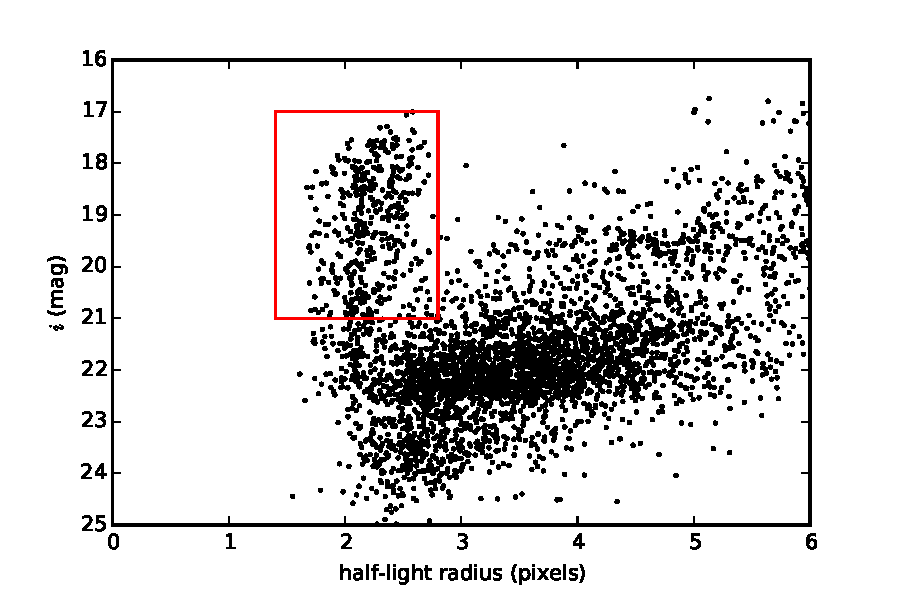
\includegraphics[width=0.8\linewidth]{figures/morph.pdf}
  \caption{Half-light radius vs.\ magnitude.}
  \label{fig:morph}
\end{figure}

\begin{figure}[htp]
  \centering
  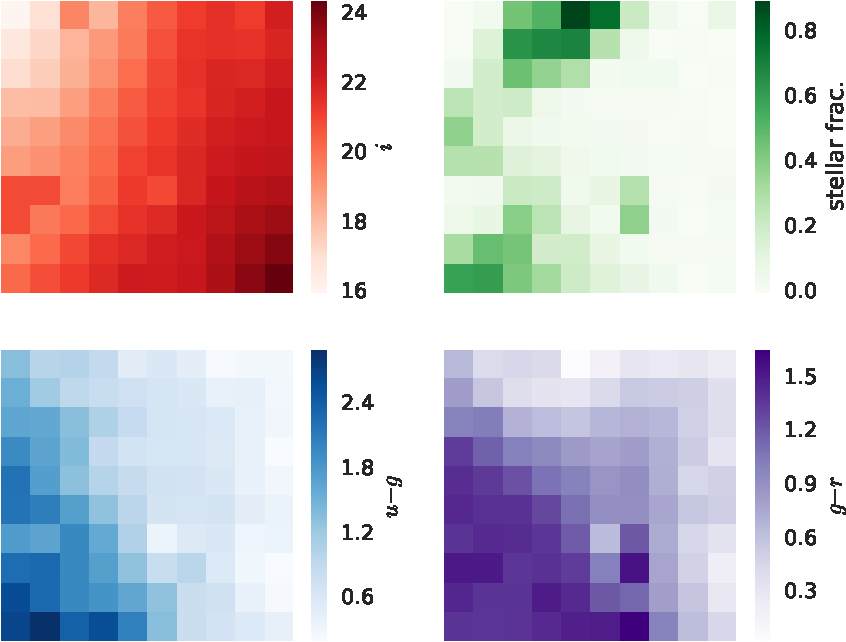
\includegraphics[width=0.7\linewidth]{figures/som_colors.pdf}
  \caption{A two-dimensional 10$\times$10 SOM representation
           showing the mean $i$-band magnitude (top left),
           the fraction of true stars in each cell (top right),
           and the mean values of $u-g$ (bottom left) and $g-r$ (bottom right)
           for the cross-validation data.}
  \label{fig:som_colors}
\end{figure}

\begin{figure}[htp]
  \centering
  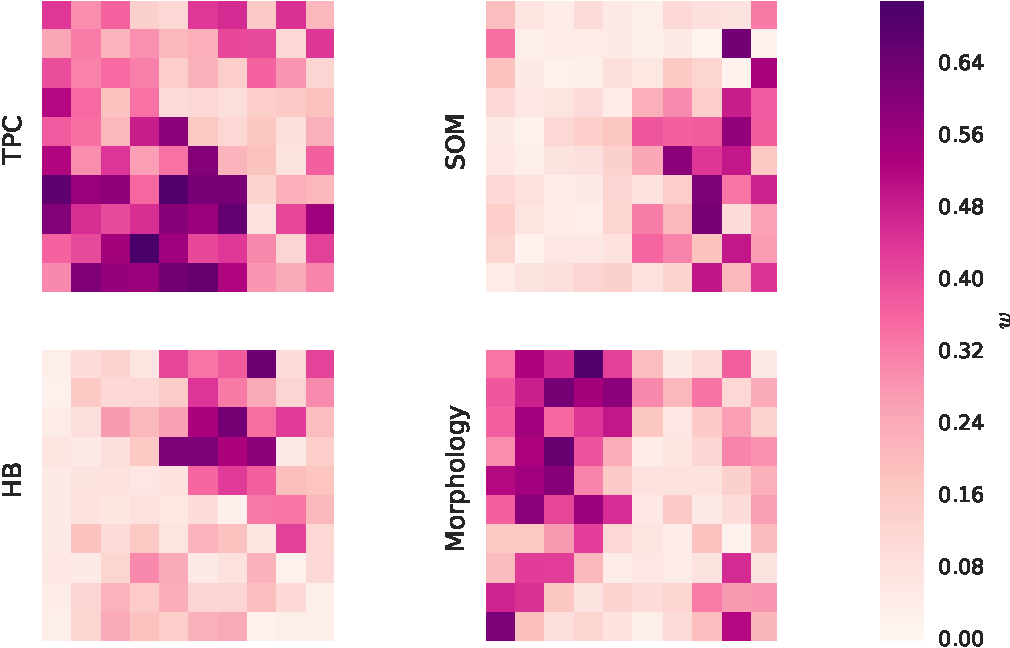
\includegraphics[width=0.8\linewidth]{figures/weights.pdf}
  \caption{A two-dimensional 10$\times$10 SOM representation
           showing the relative weights for the BMC combination technique
           applied to the four individual methods for the CFHTLenS data.}
  \label{fig:weights}
\end{figure}

\begin{figure}[htp]
  \centering
  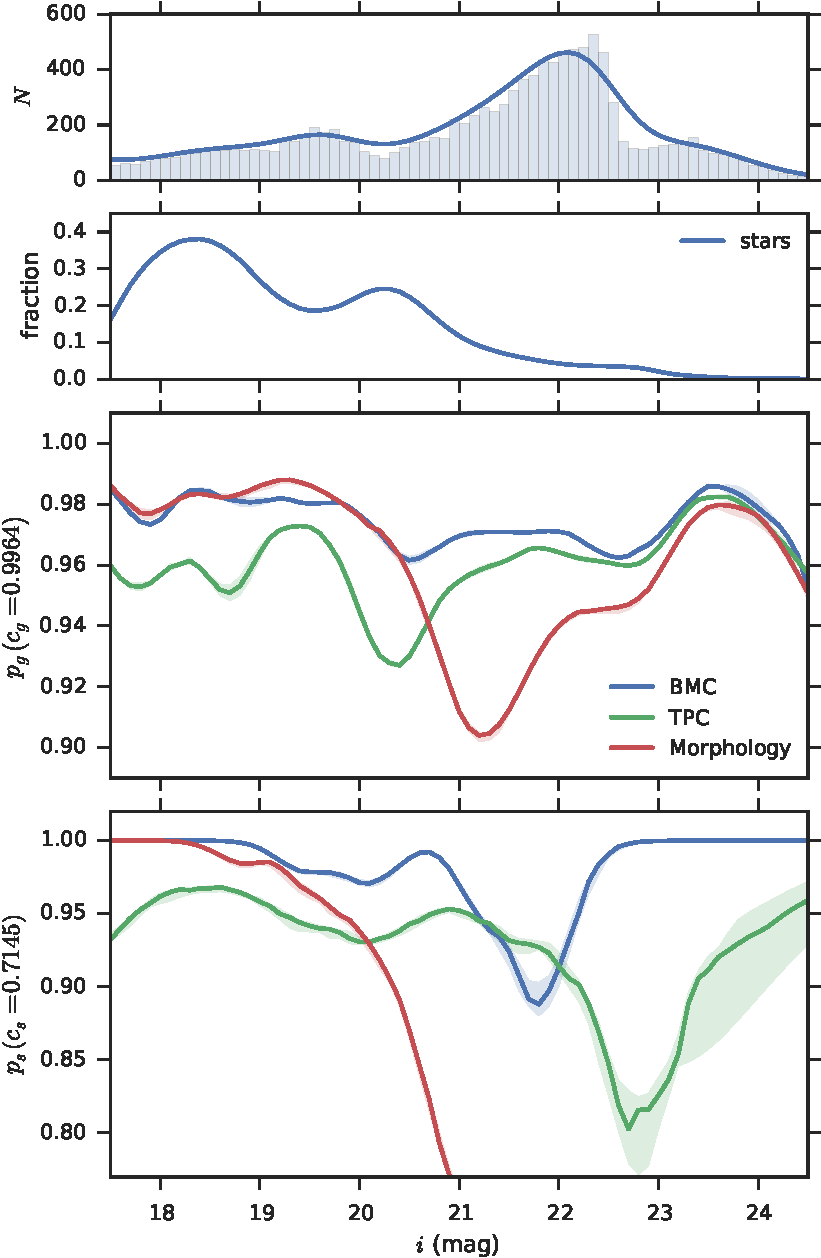
\includegraphics[width=0.7\linewidth]{figures/purity_mag.pdf}
  \caption{Purity as a function of the $i$-band magnitude
           as estimated by the kernel density estimation (KDE) method.
           The top panel shows the histogram with a bin size of 0.1 mag
           and the KDE for objects in the test set.
           The second panel shows the fraction of stars estimated by KDE
           as a function of magnitude.
           The bottom two panels compare
           the galaxy and star purity values for BMC, TPC, and 
           morphological separation as functions of magnitude.
           Results for BMC, TPC, and morphological separation are in
           blue, green, and red, respectively.
           The $1 \sigma$ confidence bands are estimated by
           bootstrap sampling.}
  \label{fig:purity_mag}
\end{figure}


\begin{figure}[htp]
  \centering
  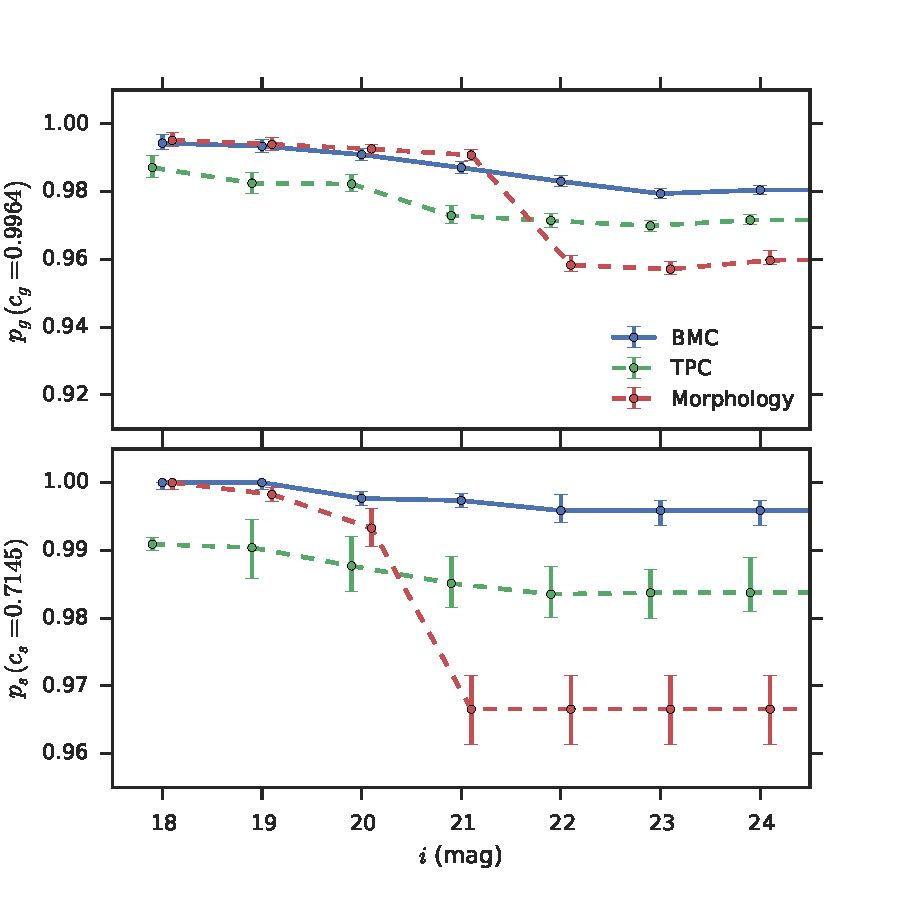
\includegraphics[width=0.8\linewidth]{figures/purity_mag_integrated.pdf}
  \caption{Cumulative purity as a function of the $i$-band magnitude.
           The upper panel compares
           the galaxy purity values for BMC (blue solid line),
           TPC (green dashed line), and 
           morphological separation (red dashed line).
           The lower panel compares the star purity.
           The $1 \sigma$ error bars are computed following the method
           of \citet{paterno2004calculating} to avoid the unphysical
           errors of binomial or Poisson statistics.}
  \label{fig:purity_mag_integrated}
\end{figure}

\begin{figure}[htp]
  \centering
  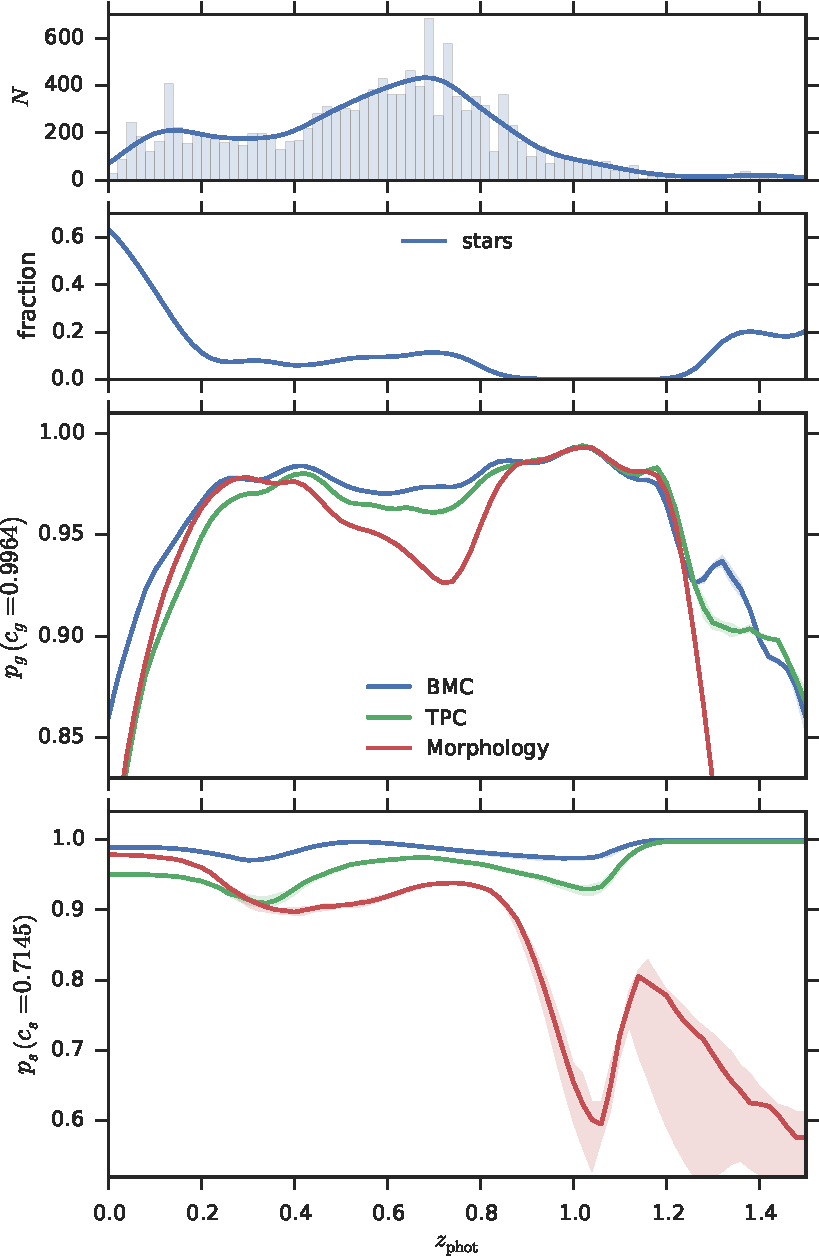
\includegraphics[width=0.7\linewidth]{figures/purity_z.pdf}
  \caption{Similar to Figure~\ref{fig:purity_mag}
           but as a function of photo-$z$.
           The bin size of histogram in the top panel is 0.02.}
  \label{fig:purity_z}
\end{figure}

\begin{figure}[htp]
  \centering
  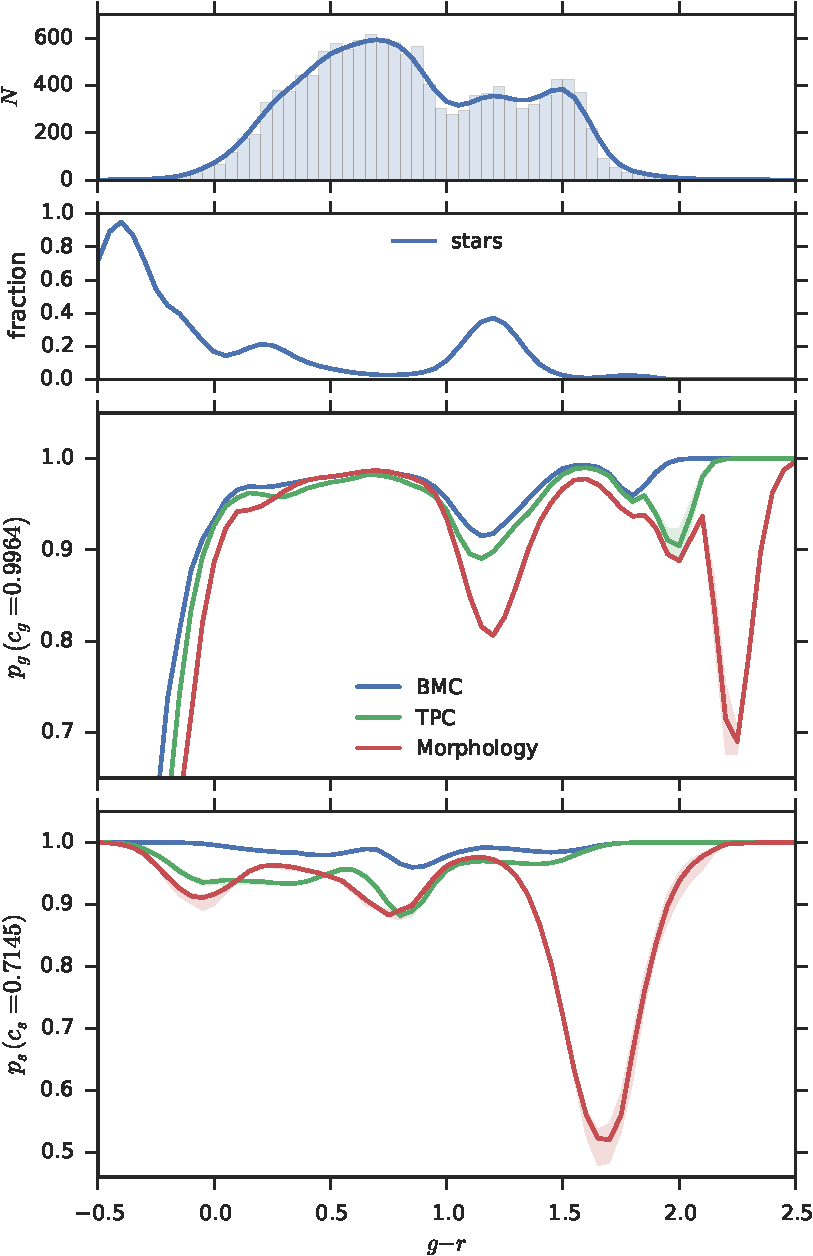
\includegraphics[width=0.7\linewidth]{figures/purity_g_r.pdf}
  \caption{Similar to Figure~\ref{fig:purity_mag}
           but as a function of $g-r$ color.
           The bin size of histogram in the top panel is 0.05.}
  \label{fig:purity_g_r}
\end{figure}

\begin{figure}[htp]
  \centering
  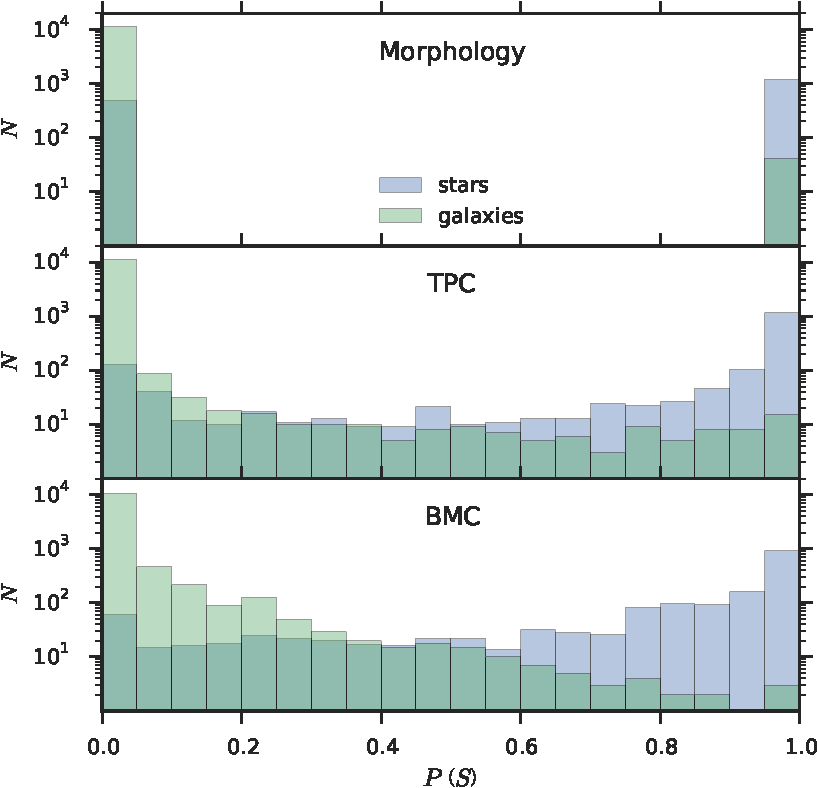
\includegraphics[width=0.7\linewidth]{figures/p_dist.pdf}
  \caption{Histogram of the posterior probability that
           a source is a star for morphological separation (top),
           TPC (middle), and BMC (bottom)
           for a high-quality training data set.
           The true galaxies are in green, and true stars are in blue.
           The bin size is 0.05.}
  \label{fig:p_dist_all}
\end{figure}


\begin{figure}[htp]
  \centering
  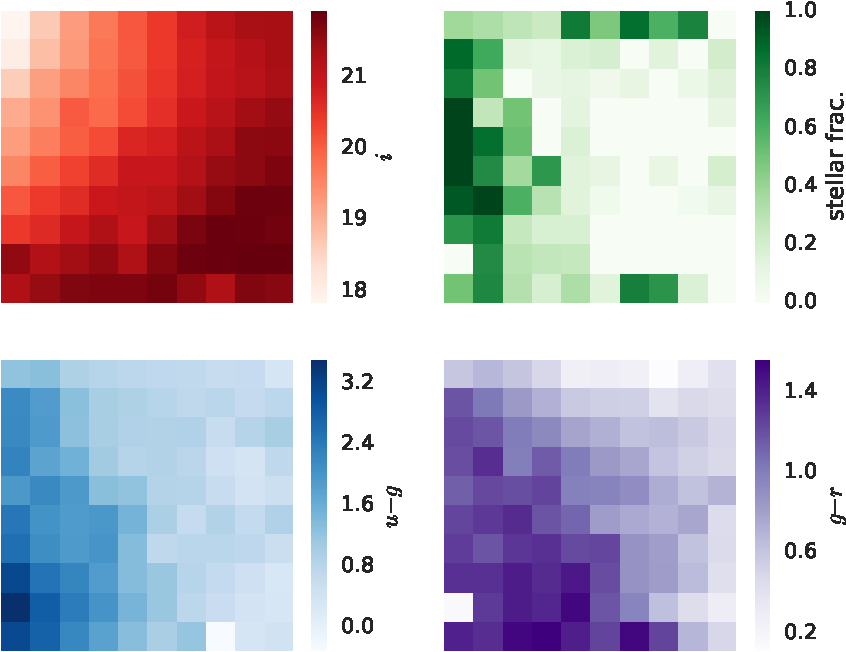
\includegraphics[width=0.7\linewidth]{figures/som_colors_cut.pdf}
  \caption{Similar to Figure~\ref{fig:som_colors}
           but for the reduced training data set. }
  \label{fig:som_colors_cut}
\end{figure}

\begin{figure}[htp]
  \centering
  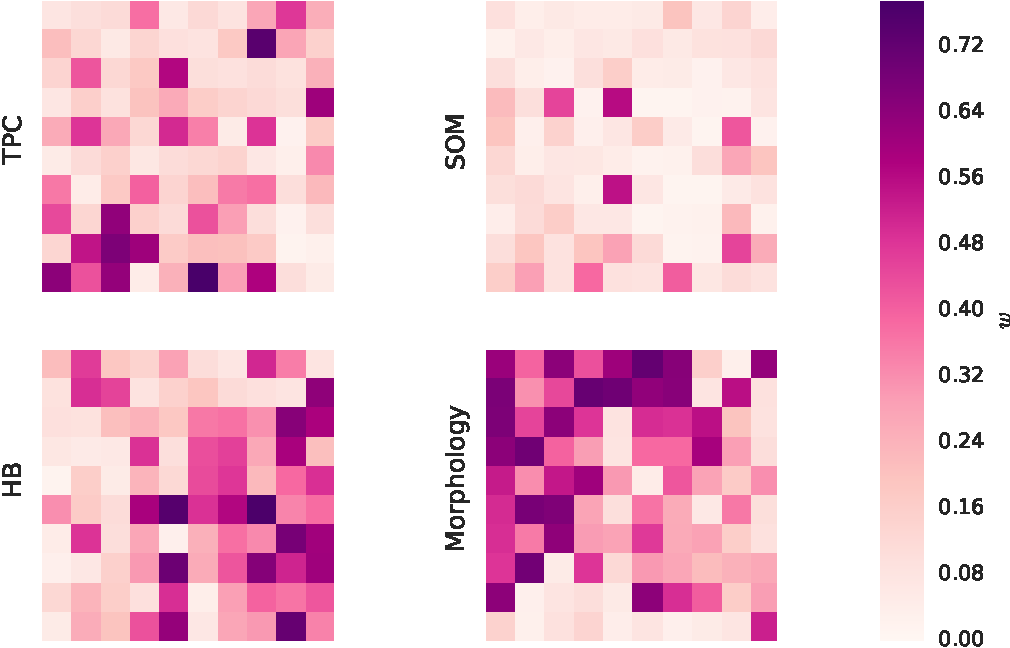
\includegraphics[width=0.8\linewidth]{figures/weights_cut.pdf}
  \caption{Similar to Figure~\ref{fig:weights}
           but for the reduced training data set. }
  \label{fig:weights_cut}
\end{figure}

\begin{figure}[htp]
  \centering
  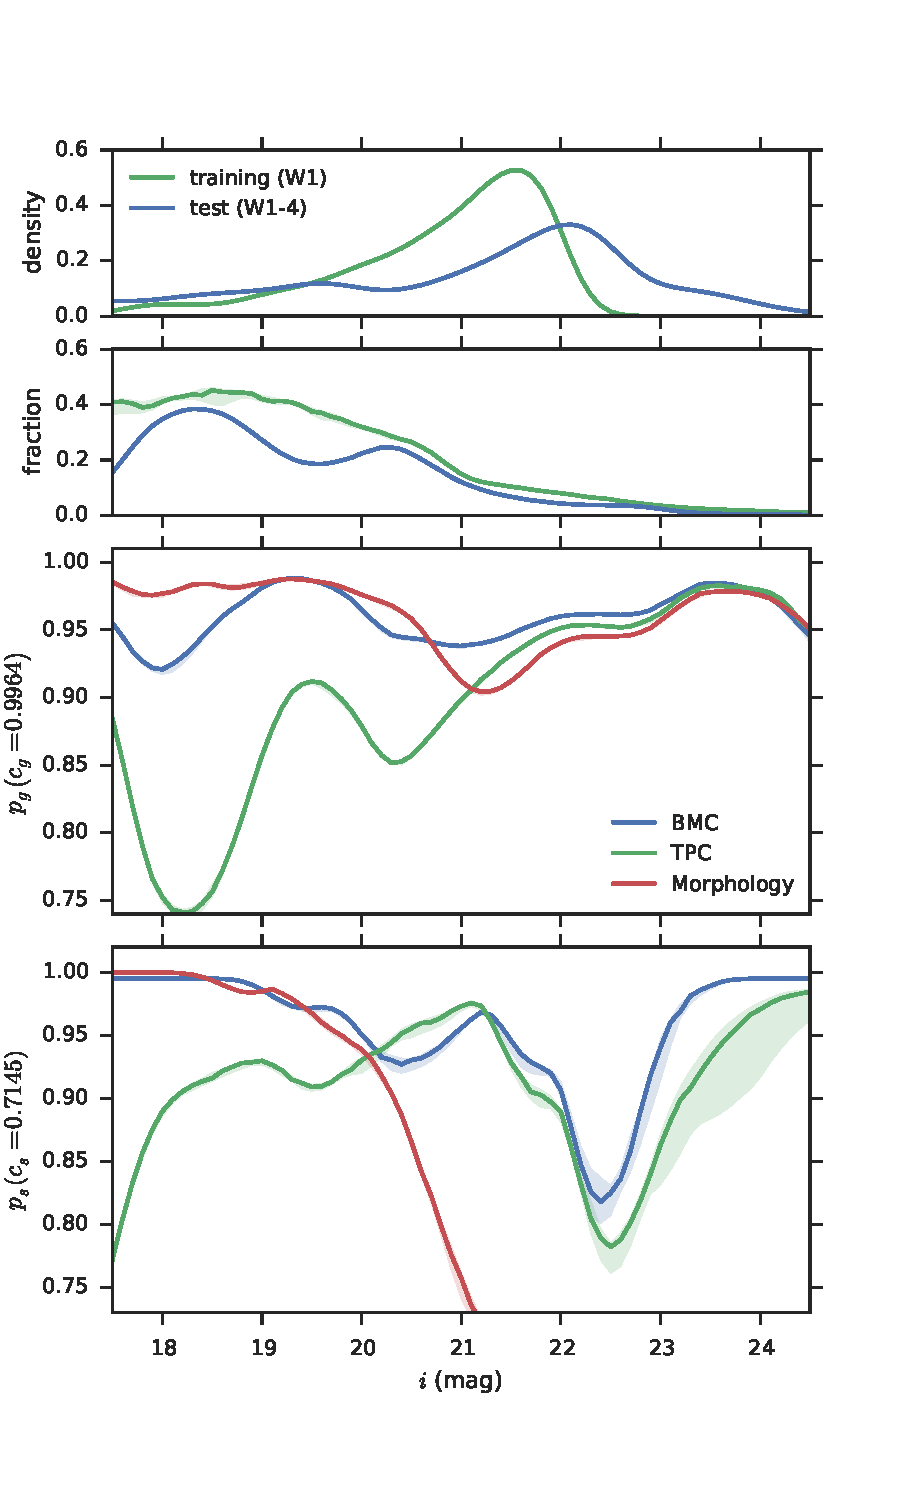
\includegraphics[width=0.7\linewidth]{figures/purity_mag_cut.pdf}
  \caption{Purity as a function of the $i$-band magnitude
           for the reduced training data set.
           Top panel shows the histograms and KDEs
           for the number count distribution for
           the training (blue) and test (green) data set.
           The second panel shows the fraction of stars
           in the training and test data set in blue and green, respectively.
           The bottom two panels compare
           the galaxy and star purity values for BMC, TPC, 
           and morphological separation as functions of $i$-band magnitude.}
  \label{fig:purity_mag_cut}
\end{figure}


\begin{figure}[htp]
  \centering
  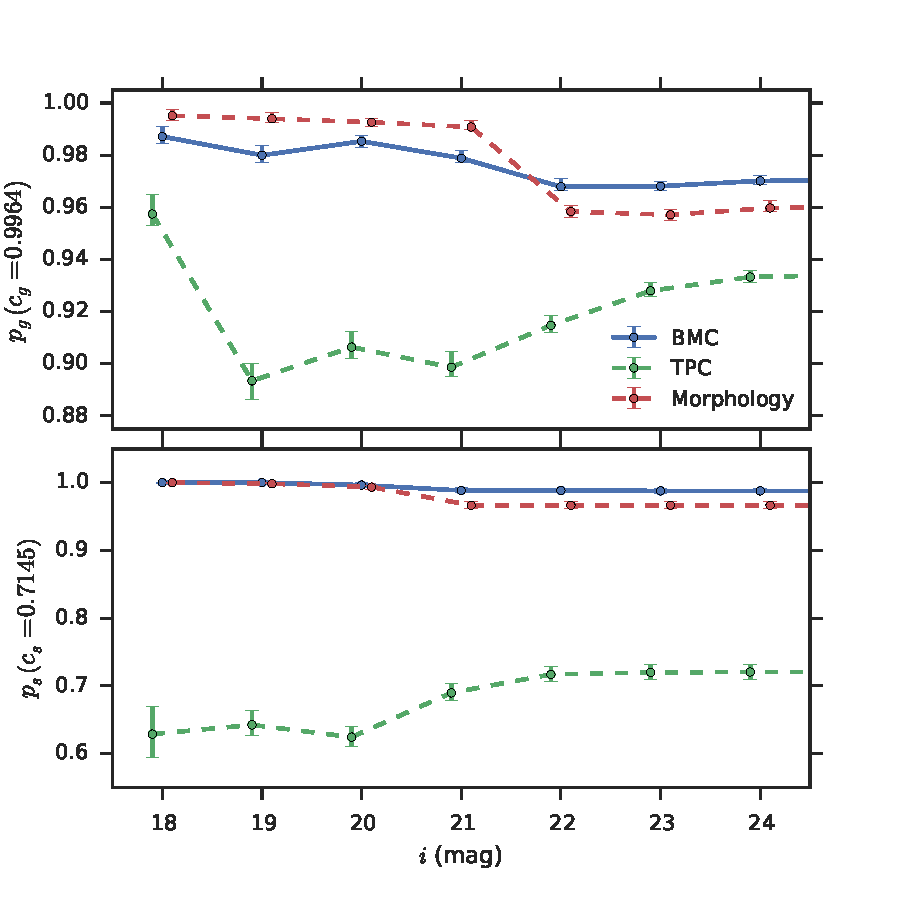
\includegraphics[width=0.8\linewidth]{figures/purity_mag_cut_integrated.pdf}
  \caption{Similar to Figure~\ref{fig:purity_mag_integrated}
           but for the reduced training data set.}
  \label{fig:purity_mag_cut_integrated}
\end{figure}

\begin{figure}[htp]
  \centering
  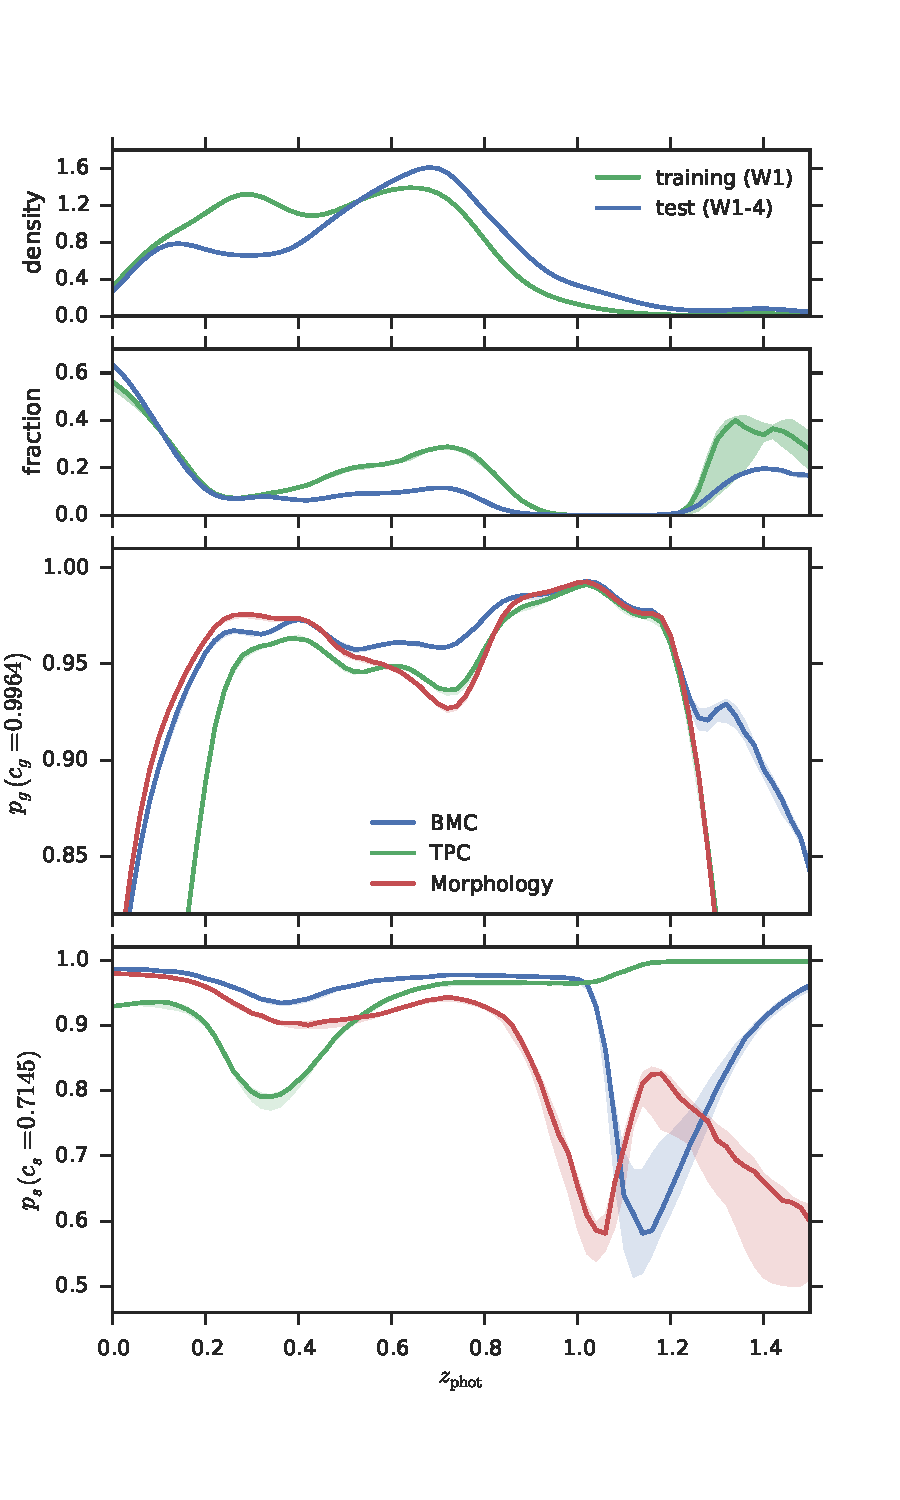
\includegraphics[width=0.7\linewidth]{figures/purity_z_cut.pdf}
  \caption{Similar to Figure~\ref{fig:purity_mag_cut}
           but as a function of photo-$z$.}
  \label{fig:purity_z_cut}
\end{figure}

\begin{figure}[htp]
  \centering
  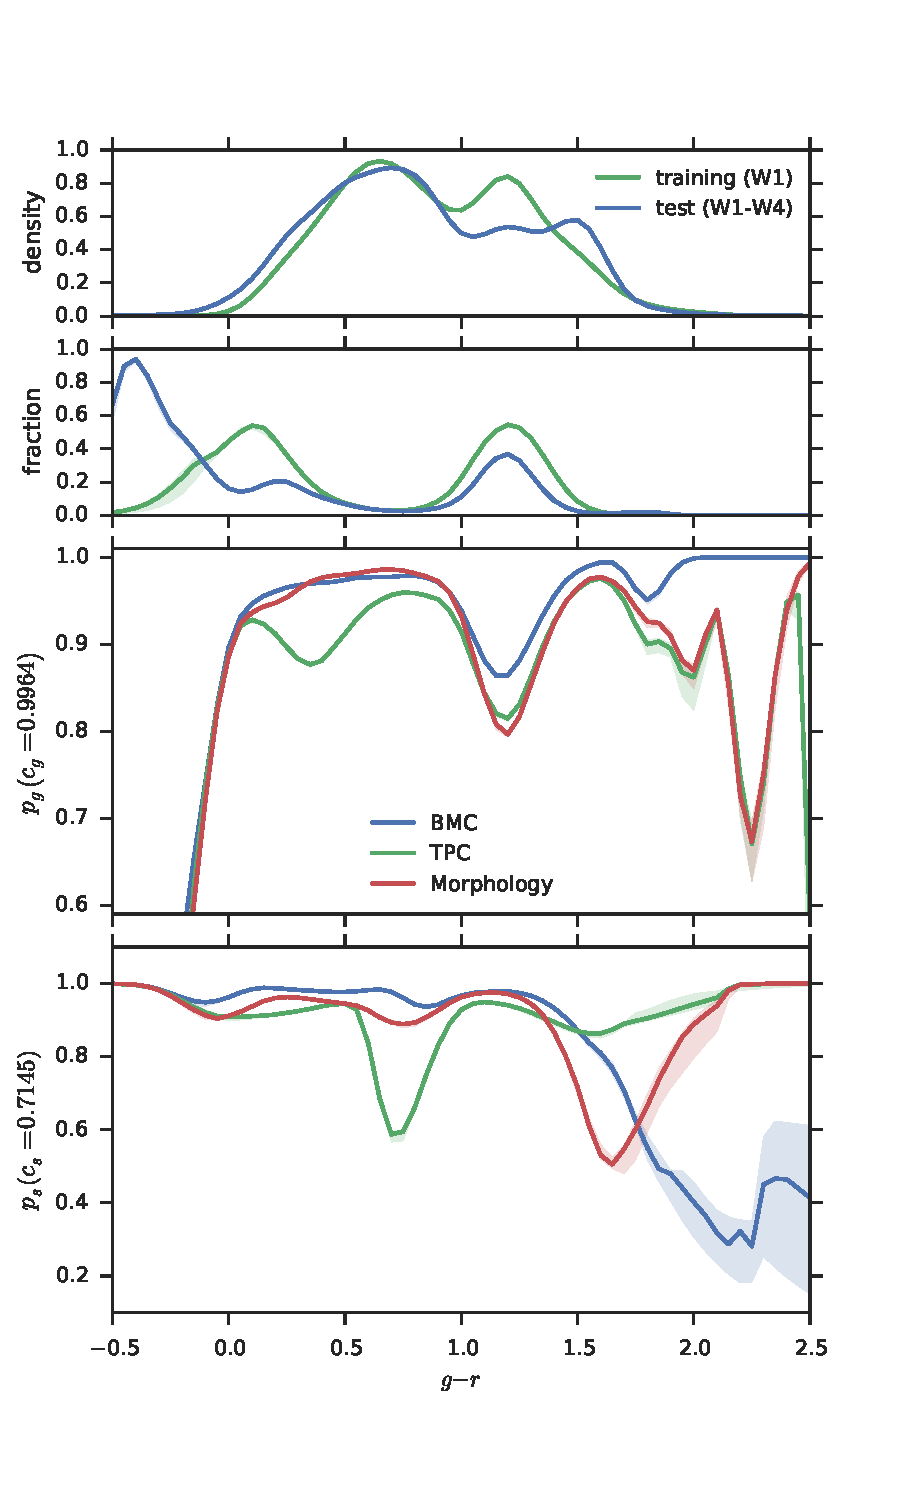
\includegraphics[width=0.7\linewidth]{figures/purity_g_r_cut.pdf}
  \caption{Similar to Figure~\ref{fig:purity_mag_cut}
           but as a function of $g-r$ color.}
  \label{fig:purity_g_r_cut}
\end{figure}

\begin{figure}[htp]
    \centering
  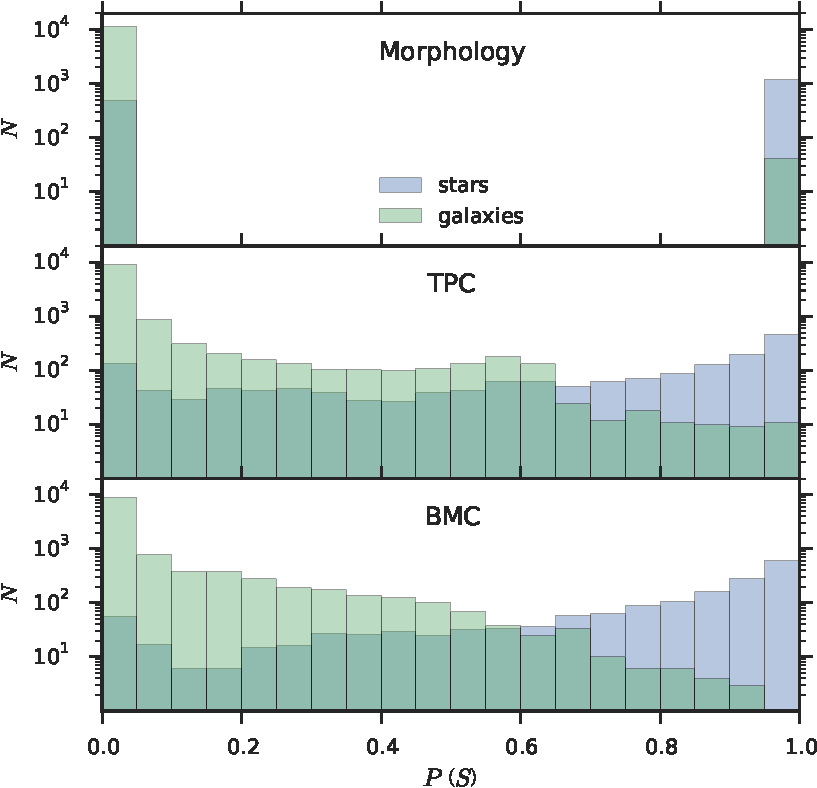
\includegraphics[width=0.7\linewidth]{figures/p_dist_cut.pdf}
  \caption{Similar to Figure~\ref{fig:p_dist_all}
           but for the reduced training data set.}
  \label{fig:p_dist_cut}
\end{figure}

\begin{figure}[htp]
    \centering
    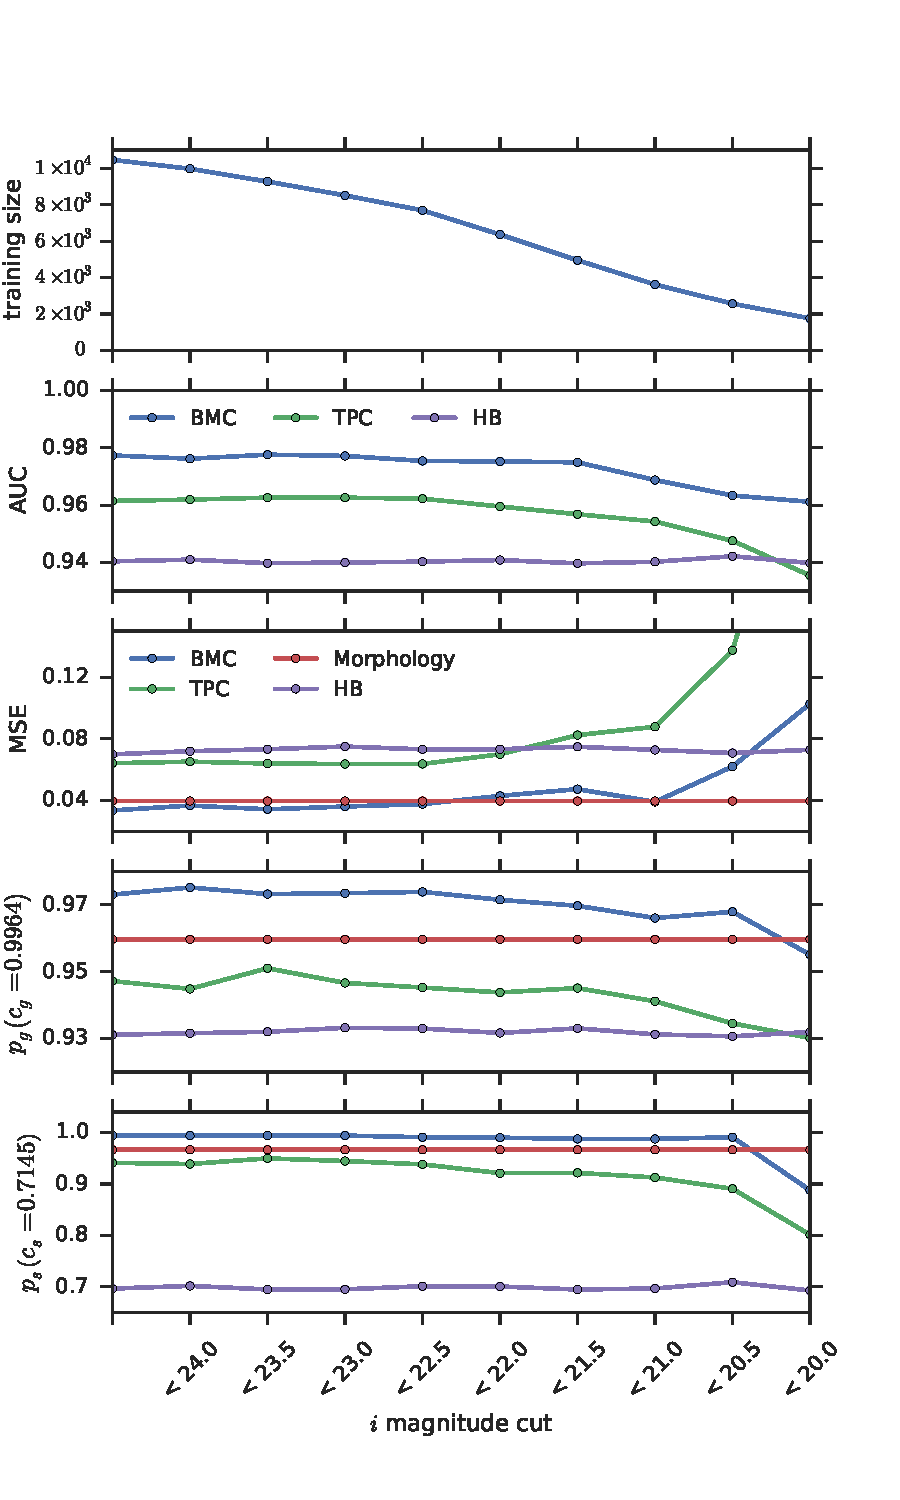
\includegraphics[width=0.7\linewidth]{figures/perform_mag_cut.pdf}
    \caption{The classification performance metrics for
      BMC (blue), TPC (green), morphology (red), and HB (purple)
      as applied to the CFHTLenS data in the VVDS field
      with various magnitude cuts.
      The top panel shows the number of sources in the training set
      at corresponding magnitude cuts.
      We show only one of the four combination methods, BMC,
      which has the best overall performance.}
    \label{fig:perform_mag_cut}
\end{figure}

\begin{figure}[htp]
    \centering
    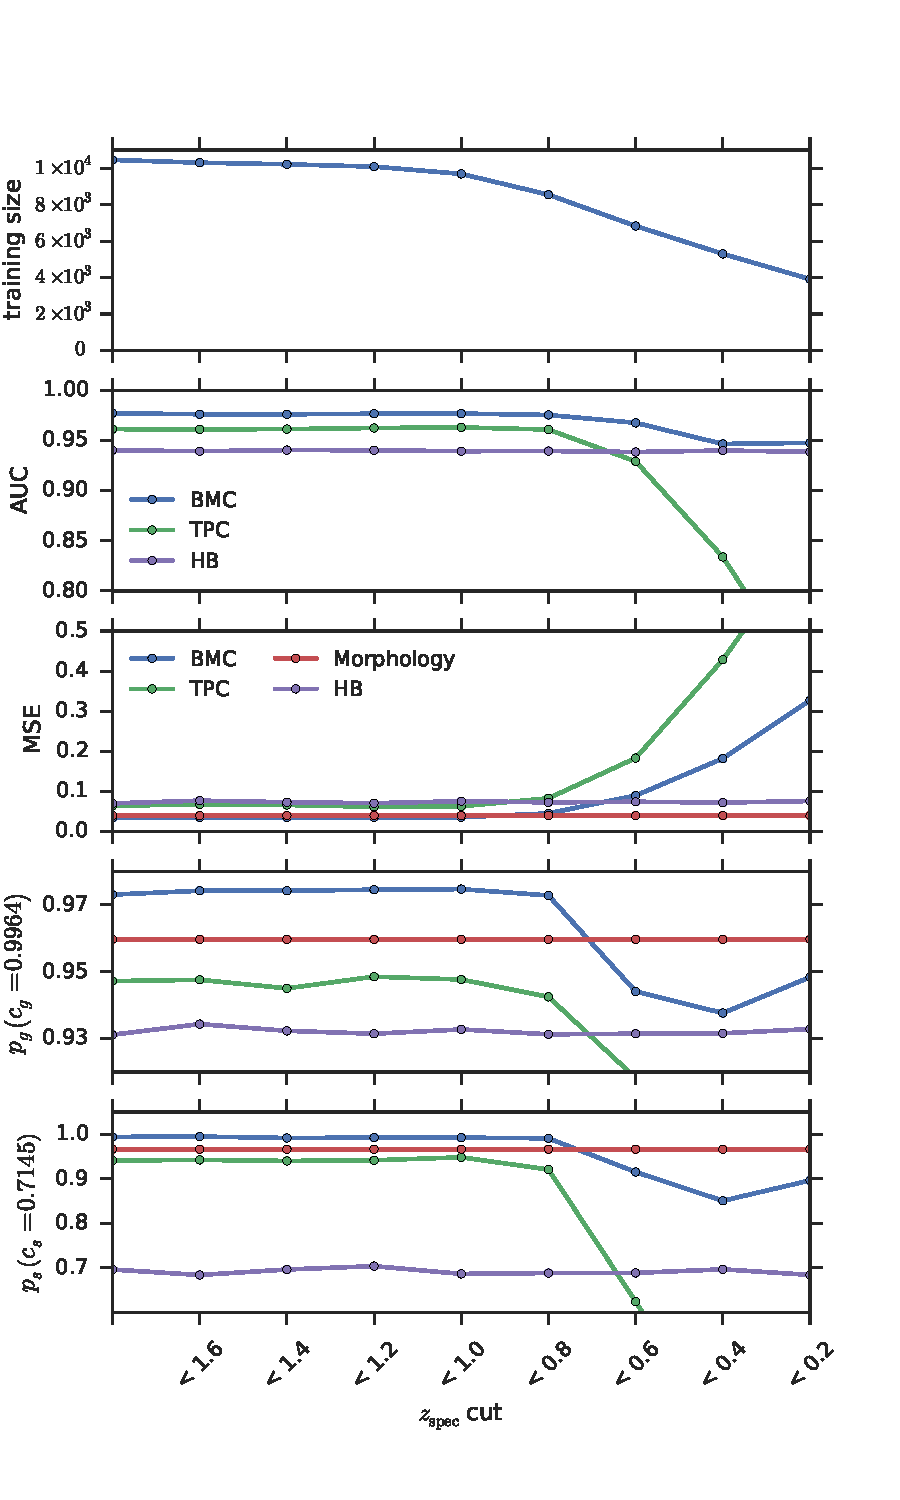
\includegraphics[width=0.7\linewidth]{figures/perform_z_cut.pdf}
    \caption{Similar to Figure~\ref{fig:perform_mag_cut}
        but using $z_{\text{spec}}$ cuts.}
    \label{fig:perform_z_cut}
\end{figure}


\begin{figure}[htp]
    \centering
    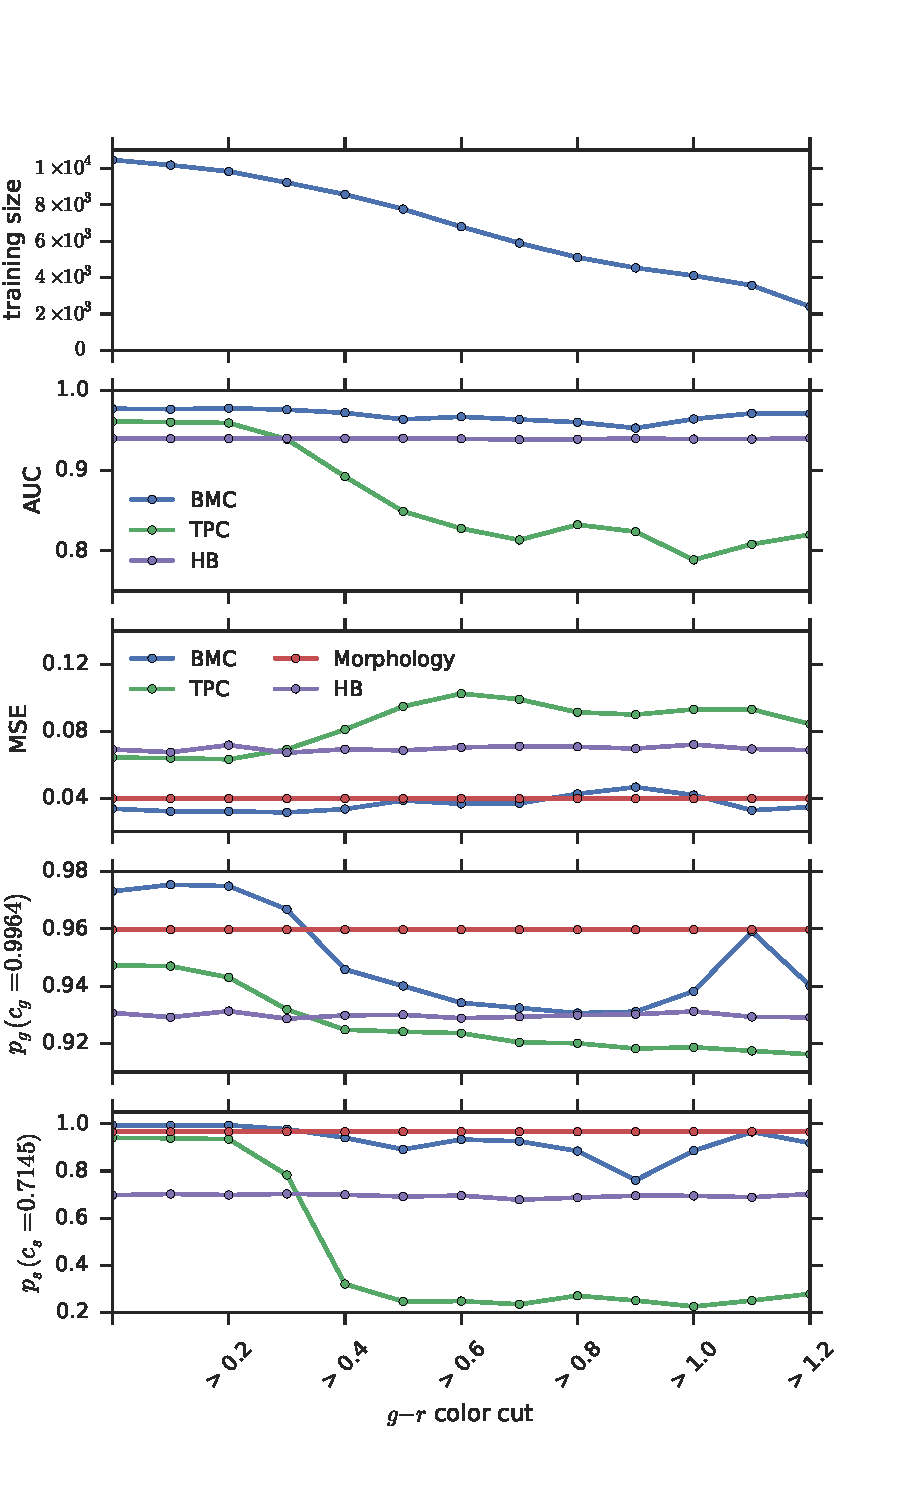
\includegraphics[width=0.7\linewidth]{figures/perform_g_r_cut.pdf}
    \caption{Similar to Figure~\ref{fig:perform_mag_cut}
        but using $g - r$ color cuts.}
    \label{fig:perform_g_r_cut}
\end{figure}

\clearpage
\begin{table}
  \centering
  \begin{tabular}{| c | l |}
  \hline
  Metric & Meaning \\
  \hline
  AUC & Area under the Receiver Operating Curve \\
  MSE & Mean squared error \\
  $c_g$ & Galaxy completeness \\
  $p_g$ & Galaxy purity \\
  $c_s$ & Star completeness \\
  $p_s$ & Star purity \\
  $p_g(c_g=x)$ & Galaxy purity at $x$ galaxy completeness \\
  $p_s(c_s=x)$ & Star purity at $x$ star completeness \\
  \hline
  \end{tabular}
  \caption{The definition of the classification performance metrics.}
  \label{table:metrics}
\end{table}

%% rich training data
\begin{sidewaystable*}
  \begin{tabular}{| l | c | c | c | c | c | c |}
  \hline
    Classifier & AUC & MSE &
    $p_{g}\left(c_g=0.9964\right)$ & $p_{s}\left(c_s=0.7145\right)$ &
    $p_{g}\left(c_g=0.9600\right)$ & $p_{s}\left(c_s=0.2500\right)$ \\
    \hline
    TPC        & \textbf{0.9870} & 0.0208 & 0.9714 & 0.9838 & 0.9918 & 0.9977 \\
    SOMc       & 0.9683 & 0.0452 & 0.9125 & 0.8454 & 0.9788 & 0.9551 \\
    HB         & 0.9403 & 0.0705 & 0.9219 & 0.7017 & 0.9471 & 0.6963 \\
    Morphology & - & 0.0397 & 0.9597 & 0.9666 & - & - \\
    WA         & 0.9806 & 0.0266 & 0.9755 & 0.9926 & 0.9872 & 0.9977 \\
    BoM        & 0.9870 & 0.0208 & 0.9714 & 0.9838 & 0.9918 & 0.9977 \\
    Stacking   & 0.9842 & 0.0194 & 0.9752 & 0.9902 & 0.9918 & \textbf{1.0000} \\
    BMC        & 0.9852 & \textbf{0.0174} & \textbf{0.9800} & $\textbf{0.9959}$ &
    $\textbf{0.9924}$ & \textbf{1.0000} \\
  \hline
  \end{tabular}
  \caption{A summary of the classification performance metrics
           for the four individual methods
           and the four different classification combination methods
           as applied to the CFHTLenS data,
           with no cut applied to the training data set.
           The definition of the metrics is summarized in
           Table~\ref{table:metrics}.
           The bold entries highlight the best performance values
           within each column.
           Note that some objects in the test set have bad or missing
           values (\eg $-99$ or $99$) in one or more attributes,
           which are included here (but are omitted, for example,
           in Figure~\ref{fig:purity_mag_integrated} when the corrsponding
           attribute is not available.)}
  \centering
  \label{table:metrics_all}
\end{sidewaystable*}

\begin{sidewaystable*}
  \begin{tabular}{| l | c | c | c | c | c | c |}
  \hline
    Classifier & AUC & MSE &
    $p_{g}\left(c_g=0.9964\right)$ & $p_{s}\left(c_s=0.7145\right)$ &
    $p_{g}\left(c_g=0.9600\right)$ & $p_{s}\left(c_s=0.2500\right)$ \\
    \hline
    TPC        & 0.9399 & 0.0511 & 0.9350 & 0.7060 & 0.9570 & 0.9747 \\
    SOMc       & 0.8861 & 0.0989 & 0.8843 & 0.4316 & 0.9165 & 0.6263 \\
    HB         & 0.9386 & 0.0760 & 0.9325 & 0.6911 & 0.9424 & 0.6918 \\
    Morphology & - & 0.0397 & 0.9597 & 0.9666 & - & - \\
    WA         & 0.9600 & 0.0536 & 0.9208 & 0.8818 & 0.9757 & 0.9815 \\
    BoM        & 0.9587 & 0.1511 & 0.9658 & 0.9862 & 0.9790 & 0.9977 \\
    Stacking   & 0.9442 & 0.1847 & 0.9561 & 0.9309 & 0.9664 & 0.9983 \\
    BMC        & \textbf{0.9738} & \textbf{0.0291} & \textbf{0.9696} & $\textbf{0.9862}$ & $\textbf{0.9856}$ & \textbf{1.0000} \\
  \hline
  \end{tabular}
  \caption{A summary of the classification performance metrics
           for the four individual methods
           and the four different classification combination methods
           when the training data set consists of
           only the sources that are in CFHTLS W1 field,
           has spectroscopic labels available from VVDS,
           and has $i < 22$.
           The definition of the metrics is summarized in
           Table~\ref{table:metrics}.
           The bold entries highlight the best performance values
           within each column.
           Note that some objects in the test set have bad or missing
           values (\eg $-99$ or $99$) in one or more attributes,
           which are included here (but are omitted, for example,
           in Figure~\ref{fig:purity_mag_cut_integrated} when the corrsponding
           attribute is not available.)}
  \centering
  \label{table:metrics_cut}
\end{sidewaystable*}


\clearpage
\bibliographystyle{plainnat}
\bibliography{thesisbib}
\chapter{Star-galaxy Classification Using Deep Convolutional Neural Networks}
  \label{chapter3}


\blfootnote{
This chapter contains material from the following previously published article:
\nobibliography{thesisbib}
\begin{itemize}
\item\bibentry{kim2017star}
\end{itemize}
}

\section{Introduction}
  \label{sec:introduction}

Currently ongoing and forthcoming large-scale photometric surveys,
such as the Dark Energy Survey (DES) and the Large Synoptic Survey Telescope (LSST),
aim to collect photometric data for hundreds of millions to billions of
stars and galaxies.
Due to the sheer volume of data, it is not possible for human experts to
manually classify them,
and the separation of photometric catalogs into stars and galaxies has to be automated.
Furthermore, any classification approach must be probabilistic in nature.
A fully probabilistic classifier enables a user to adopt probability cuts
to obtain a pure sample for population studies,
or to optimize the allocation of observing time by selecting objects for follow-up.
Ideally, however, the probability estimates themselves would be retained for all sources
and used in subsequent analyses to improve or enhance a particular
measurement~\citep{ross2011ameliorating,seo2012acoustic}.

With machine learning, we can use algorithms to automatically create
accurate source catalogs with well-calibrated posterior probabilities.
Machine learning techniques have been a popular tool
in many areas of astronomy~\citep{ball2008robust,
banerji2010galaxy,
carrascokind2013tpz,
ivezic2014statistics,
kamdar2016machine1}. 
Artificial neural networks were first applied to the problem of star-galaxy
classification in the work of \citet{odewahn1992automated},
and they have become a core part of the astronomical image processing software
\texttt{SExtractor}~\citep{bertin1996sextractor}.
Other successfully implemented examples of applying machine learning to
the star-galaxy classification problem include decision 
trees~\citep{weir1995automated,suchkov2005census,ball2006robust,vasconcellos2011decision,sevilla2015effect}, 
Support Vector Machines~\citep{Fadely2012}, and
classifier combination strategies~\citep*{kim2015hybrid}.

Almost all star-galaxy classifiers published in the literature use
the reduced summary information available from astronomical catalogs.
Constructing catalogs requires careful engineering and considerable domain expertise
to transform the reduced, calibrated pixel values that comprise an image into suitable features,
such as magnitudes or shape information of an object.
In a branch of machine learning called \textit{deep learning}~\citep{lecun2015deep},
features are not designed by human experts;
they are learned directly from data by deep neural networks.
Deep learning methods learn multiple levels of features by
transforming the feature at one level into a more abstract feature at a higher
level.
For example, when an array of pixel values is used as input to a deep learning
method, the features in the first layer might represent locations and orientations
of edges.
The second layer could assemble particular arrangements of edges into more
complex shapes, and subsequent layers would detect objects as
combinations of low-level features.
These multiple layers of abstraction progressively amplify aspects of the input
that are important for classification tasks.
Deep learning has been applied successfully to galaxy morphological
classification in Sloan Digital Sky Survey~\citep[SDSS;][]{dieleman2015rotation}
and Cosmic Assembly Near-infrared Deep Extragalactic Legacy
Survey~\citep[CANDELS;][]{huertas2015catalog} and to photometric redshift
estimation~\citep{hoyle2015measuring},
but it has not yet been applied to the problem of source classification.

In this chapter, we present a star-galaxy classification framework
that uses a convolutional neural network (ConvNet) model directly on the images
from the SDSS and the Canada-France-Hawaii Telescope Lensing Survey (CFHTLenS).
We compare its performance with a standard machine learning technique
that uses the reduced summary information from catalogs,
and we demonstrate that our ConvNet model is able to produce accurate and
well-calibrated probabilistic classifications with very little feature
engineering by hand.
In Section~\ref{sec:data}, we describe the data sets used in this work
and the pre-processing steps for preparing the image data sets.
We provide a brief overview of deep learning and ConvNets
in Section~\ref{sec:deep_learning}, and
discuss our strategy for preventing overfitting in Section~\ref{sec:overfitting}.
In Section~\ref{sec:tpc}, we describe a state-of-the-art tree-based
machine learning algorithm, to which the performance of our ConvNet model is
compared.
We present the main results of our ConvNet model in
Section~\ref{sec:results_and_discussion}, and
we outline our conclusions in Section~\ref{sec:conclusions}.

\section{Data}
  \label{sec:data}

To demonstrate the performance of our ConvNet model, we use photometric and
spectroscopic data sets with different characteristics and compositions.
In this section, we briefly describe these data sets and the image pre-processing
steps for retrieving cutout images.

\subsection{Sloan Digital Sky Survey}
  \label{sec:sdss}

The Sloan Digital Sky Survey~\citep[SDSS;][]{york2000sloan}
phases I--III obtained photometric data in five bands,
$u$, $g$, $r$, $i$, and $z$,
covering 14,555 square degrees, more than one-third of the entire sky.
The resulting catalog contains photometry of over 300 million stars and galaxies
with a limiting magnitude of $r \approx 22$,
making the SDSS one of the largest sky surveys ever undertaken.
The SDSS also conducted an expansive spectroscopic follow-up of
more than three million stars and galaxies~\citep{eisenstein2011sdss}.
In this work, we use a subset of the photometric and spectroscopic data
contained within the Data Release 12~\citep[DR12;][]{alam2015eleventh},
which is publicly available through the online CasJobs server \citep{li2008casjobs}.

Using the CasJobs server, we randomly select a total of 65,000 sources,
which are either stars or galaxies.
In this work, we exclude objects that clearly are neither stars nor galaxies.
Most of the excluded objects are QSOs or quasars.
Quasars appear as point sources, rather than resolved sources similar to
galaxies,
and many of them have one or more saturated pixels in the images.
However, unlike any known stars, their spectra show strong and broad emission
lines.
Quasars are also different from galaxies because of their intrinsic variability
on a wide range of time scales, which may be due to variation in the accretion
rate or instabilities of the accretion disk around the black hole
\citep{popovic2012photocentric}.
Thus, many studies exclude quasars in the binary star-galaxy classification
scheme~\citep[\eg][]{vasconcellos2011decision,Fadely2012}.
Expanding the historical star-galaxy classification problem to include
additional classes, \eg \textit{nsng} (neither star nor galaxy),
may have advantages~\citep{ball2006robust}.

We also exclude some bad photometric observations as follows.
We consider only objects
with no warning flags in the spectroscopic measurement (\texttt{zWarning = 0});
the half-light radius in the $r$ band is less than 30 arc seconds
as measured by the exponential and de Vaucouleurs light profiles;
the error on the spectroscopic redshift measurement is less than 0.1; and
the spectroscopic redshift is less than 2.

To create training images,
we obtain the image FITS files for SDSS fields containing these objects
in five photometric bands: $u$, $g$, $r$, $i$, and $z$.
We use the astrometry information in the FITS headers
in the \texttt{Montage} software to align each image to the reference ($r$-band) image.
We then use \texttt{SExtractor} to find the pixel positions of
the 65,000 objects we have selected,
and to center each object in the cutout image.
Magnitudes in the SDSS photometric catalog are expressed as inverse hyperbolic
sine magnitudes~\citep[also known as luptitudes;][]{lupton1999modified},
and we follow the SDSS convention and convert all flux values to luptitudes.
Finally, in order to account for the effect of Galactic dust,
extinction corrections in magnitudes are applied
following \cite{schlegel1998maps}.
In the end, we have cutout images of size $48\times48$ pixels
with luptitude values in each pixel.
We note that we have experimented with increasing the pixel dimensions to
$60\times60$ and $72\times72$ pixels, but do not find noticeable
improvement in the performance of our model.

In the end, we have 17,344 stars and 47,656 galaxies available
for the training and testing processes.
The apparent magnitudes range from $10.7 < r < 23.1$,
and the galaxies in this sample have a mean redshift of $z \sim 0.36$.
We randomly split the objects into training, held-out validation,
and blind test sets of size 40,000, 10,000, and 15,000, respectively.
We note that cross-validation is often avoided in deep learning
in favor of hold-out validation,
since cross-validation is computationally expensive.
We also note that we perform a blind test, and the test set is not used in any
way to train or calibrate the algorithms.
The first two panels of Figure~\ref{fig:sdss_mag} show the number of objects
and the fraction of stars in the test set as functions of $r$-band magnitude.
Similarly, Figure~\ref{fig:sdss_g_r} shows the number of objects and the
fraction of stars in the test set as functions of $g-r$ color.
The normalized kernel density estimate distributions for the training
and validation sets are almost identical to those of the test set,
and they are nearly indistinguishable when overlapped.
We do not show the distributions for the training and validation sets in
Figures~\ref{fig:sdss_mag} and \ref{fig:sdss_g_r} to avoid cluttering the
plots.


\subsection{Canada-France-Hawaii Telescope Lensing Survey}

We also use photometric data from
the Canada-France-Hawaii Telescope Lensing Survey
\cite[CFHTLenS;][]
{heymans2012cfhtlens,erben2013cfhtlens,hildebrandt2012cfhtlens}.
This catalog consists of more than twenty five million objects
with a limiting magnitude of $i_{\text{AB}} \approx 25.5$. 
It covers a total of 154 square degrees
in the four fields (named W1, W2, W3, and W4)
of the CFHT Legacy Survey~\citep[CFHTLS;][]{gwyn2012canada}
observed in the five photometric bands:
$u$, $g$, $r$, $i$, and $z$.

We have cross-matched reliable spectroscopic galaxies from
the Deep Extragalactic Evolutionary Probe Phase 2~
\citep[DEEP2;][]{davis2003science,newman2013deep2},
the Sloan Digital Sky Survey Data Release 10~\citep[SDSS-DR10]{alam2015eleventh},
the VIsible imaging Multi-Object Spectrograph (VIMOS)
Very Large Telescope (VLT) Deep Survey~
\citep[VVDS;][]{le2005vimos,garilli2008vimos}, and
the VIMOS Public Extragalactic Redshift
Survey~\citep[VIPERS;][]{garilli2014vimos}.
We have selected only sources with very secure
redshifts and no bad flags (quality flags -1, 3, and 4 for DEEP2;
quality flag 0 for SDSS; quality flags 3, 4, 23, and 24 for VIPERS
and VVDS).

We obtain FITS images for each 1 square degree CFHTLenS pointing
that contains objects with spectroscopic labels.
We create cutout images of size $96\times96$ pixels by using a similar method
to that described in Section~\ref{sec:sdss}.
Finally, images are downscaled to $48\times48$ pixels
to reduce the computational cost.

In the end, we have 8,545 stars and 57,843 galaxies available
for the training and testing processes.
The apparent magnitudes range from $13.9 < r < 25.6$,
and the galaxies in this sample have a mean redshift of $z \sim 0.59$.
We randomly split the objects into training, held-out validation, and
blind test sets of size 40,000, 10,000, and 13,278, respectively.
Figures~\ref{fig:clens_mag} and \ref{fig:clens_g_r} show the distribution
of objects in the test set as functions of $i$-band magnitude and $g-r$ color.
We do not show the distributions for the training and validation sets,
since the normalized kernel density estimate distributions for the training
and validation sets are almost identical to those of the test set.

\section{Deep Learning}
  \label{sec:deep_learning}

Neural networks have many hyperparameters, including those that specify the
network itself (\eg the size and non-linearity of each layer)
and those that specify how the network is trained
(\eg the mini-batch size or the learning rate).
Furthermore, the architecture of a neural network can have a
significant impact on its performance.
In this section, we provide a brief description of key hyperparameters in our
ConvNet model, and also present the network architecture.

\subsection{Neural Networks}

An artificial neuron in most artificial neural networks is represented
as a mathematical function that models a biological neural structure
\citep{aggarwal2014data}.
A schematic representation is shown in Figure~\ref{fig:neuron_a}.
Let $\mathbf{x}=\left(x_1,x_2,\dots,x_n\right)$ be a vector of inputs to a given neuron,
$\mathbf{w}=\left(w_1,w_2,\dots,w_n\right)$ be a vector of weights, and
$b$ be the bias.
Then, the output of the neuron is
\citep{rosenblatt1961principles}
\begin{equation}
  y = \sigma \left( \mathbf{w} \cdot \mathbf{x} + b \right),
  \label{eq:neuron_output}
\end{equation}
where $\sigma$ is the activation function (or \textit{non-linearity}).
The most popular non-linearity at present
is the rectified linear unit
\citep[ReLU;][]{nair2010rectified}, $\sigma(x)=\max(0, x)$.
ReLUs generally allow much faster
training of deep neural networks with many layers.
However, ReLU units can sometimes result in dead neurons whose output is always zero.
To mitigate this problem, we use leaky ReLUs
~\citep{maas2013rectifier}
that have a small, non-zero slope in the negative region,
\begin{equation}
  \sigma(x) =
    \begin{cases}
      x & \mbox{if } x \geq 0 \\
      0.01x & \mbox{if } x < 0.
    \end{cases}
\end{equation}

Many deep learning models use feedforward neural network architectures with multiple layers,
where each neuron in one layer is connected to the neurons of the subsequent
layer~\citep{lecun2015deep}.
A schematic representation is shown in Figure~\ref{fig:neuron_b}.
All layers except the input and output layers are conveniently called hidden layers.

We
find a set of weights and biases such that,
given $N$ samples, the output from the network
$\mathbf{y}=\left(y_1, y_2, \dots, y_N \right)$ approximates the desired output
$\hat{\mathbf{y}}=\left(\hat{y}_1, \hat{y}_2, \dots, \hat{y}_N \right)$
as closely as possible for all input
$\mathbf{X}=\left(\mathbf{x}_1,\mathbf{x}_2,\dots,\mathbf{x}_N\right)$.
We can formulate this as the minimization of a loss function
$L(\mathbf{y},\hat{\mathbf{y}})$
over the training data.
In this work, we use \textit{cross-entropy}
\citep[also called log loss;][]{murphy2012machine} as the loss function.
For binary classification, the cross-entropy per sample is given by
\begin{equation}
  L(y_j, \hat{y}_j) = -\hat{y}_j \log_2 y_j - (1 - \hat{y}_j) \log_2(1 - y_j),
  \label{eq:cross_entropy}
\end{equation}
where $\hat{y}_j$ is the actual truth value (\eg 0 or 1) of the $j$-th data, and
$y_j$ is the probability prediction made by the model.
We compute the loss function by taking the average of all cross-entropies in the sample.
Thus, the loss function becomes
\begin{equation}
  L(\mathbf{y}, \hat{\mathbf{y}})
= - \frac{1}{N} \sum_{j=1}^{N} \hat{y}_j  \log_2 y_j
    + (1 - \hat{y}_j)  \log_2 (1 - \hat y_j).
  \label{eq:cross_entropy_all}
\end{equation}

To find the weights $\mathbf{w}$ and biases $\mathbf{b}$ which minimize the loss,
we use a technique called \textit{gradient descent},
where we use the following rules to update the parameters in each layer $l$:
\begin{align}
  \mathbf{w}_l &\rightarrow
  \mathbf{w}_l^{\prime}
  = \mathbf{w}_l - \eta \frac{\partial L}{\partial \mathbf{w}_l} \nonumber \\
  \mathbf{b}_l &\rightarrow
  \mathbf{b}_l^{\prime}
  = \mathbf{b}_l - \eta \frac{\partial L}{\partial \mathbf{b}_l},
  \label{eq:gradient_descent}
\end{align}
where $\eta$ is a small, positive number known as the \textit{learning rate}.
The gradients can be computed using the backpropagation
procedure~\citep{rumelhart1988learning}.
A common approach to speed up training is to split the training data
into mini-batches~\citep{lecun1998efficient}.
In mini-batch gradient descent, instead of computing the gradients in
Equation~\ref{eq:gradient_descent} for the entire training data,
we only compute the gradient of randomly chosen training examples at each step.
As training examples are usually correlated,
the gradient computed from each mini-batch is a good approximation
of the overall gradient~\citep{bottou1998online}.
As a result, mini-batch gradient descent results in much faster convergence.
However, there is a trade-off: the lower the batch size is,
the lower the convergence rate will be;
the higher the batch size is, the longer it will take to compute the gradient
at each step~\citep{bousquet2008tradeoffs}.
Thus, a moderate batch size, combined with a decaying learning rate, is
generally used in practice. We use a batch size of 128 in this work.


We define an \textit{epoch} as a single, complete pass through the training data,
and full training usually requires many epochs.
At the end of each epoch, we evaluate the loss function on the validation set,
and the model that minimizes the validation loss is chosen as the best model.






\subsection{Convolutional Neural Networks}
  \label{sec:convnet}

The convolutional neural network~\citep[ConvNet;][]{fukushima1980neocognitron,lecun1998gradient}
is a type of deep, feedforward neural network
that has recently become
a popular
approach in the computer vision community.
In a typical ConvNet, the first few stages are composed of two types of layers: 
convolutional layers and pooling layers.

The input to a convolutional layer is an image, and the output channels of
each layer are called \textit{feature maps}.
To produce output feature maps, we convolve each feature map with a set of weights
called \textit{filters},
and apply a non-linearity such as ReLU to the weighted sum of these convolutions.
Different feature maps use different sets of filters,
but all neurons in a feature map share the same set of filters.
Mathematically, we replace the dot product in Equation~\ref{eq:neuron_output}
with a sum of convolutions. Thus, the $k$-th feature map is given by
\begin{equation}
  y^k = \sigma \left( \sum_{m} \mathbf{w}_m^k \ast \mathbf{x}_m + b^k \right),
\end{equation}
where we sum over the set of input feature maps,
$\ast$ is the convolution operator, and $\mathbf{w}_m^k$ represent the filters.

Typically, a
pooling layer computes the maximum of a local $2\times2$ patch in a feature map
\citep{krizhevsky2012imagenet}.
Since the pooling layer aggregates the activations of neighboring units from the previous layer,
it reduces the dimensionality of the feature maps and
makes the model invariant to small shifts and distortions
\citep{boureau2010theoretical}
.
Two or more layers of convolution and pooling are stacked,
followed by more convolutional and fully-connected layers.

\subsection{Neural Network Architecture}

We present the overall architecture of our ConvNet model in Table~\ref{table:hyperparamters}.
The network consists of eleven trainable layers.
The first convolutional layer filters the $5\times44\times44$ input image
(\ie $44\times44$ images in five bands $ugriz$) with 32 square filters of size $5\times5\times5$.
We have also experimented with using only three bands $gri$ (for three channels of RGB) and 
four bands $ugri$ and $griz$ (corresponding to RGBA),
and using only colors, \eg $u-g$, $g-r$, $r-i$, and/or $i-z$,
but we find that using magnitudes in all five bands $ugriz$ yields the best performance.

The leaky ReLU non-linearity is applied to the output of the first convolutional layer
(and all subsequent layers), and the second convolutional layer filters it
with 32 filters of $32\times3\times3$.
In the second convolutional layer (and all subsequent convolutional layers),
we pad the input with zeros spatially on the border
(\ie the zero-padding is 1 pixel for $3\times3$ convolutional layers)
such that the spatial resolution is preserved after convolution.
Max-pooling with filters of size $2\times2$ follows the second convolutional layer.
A stack of six additional convolutional layers, all with filters of size $3\times3$,
is followed by three fully-connected layers.
The first two fully-connected layers have 2048 channels each,
and the third performs binary classification.

The output of the final fully-connected layer is fed to a \textit{softmax} function.
The softmax function is given by
\begin{equation}
  P (G \mid \mathbf{x}) = 
    \frac{ e^{ \mathbf{x} \cdot \mathbf{w}_G } }
    { \sum_{i} e^{ \mathbf{x} \cdot \mathbf{w}_i } },
\end{equation}
where we sum over the different possible values of the class label (\ie star or galaxy),
and interpret its output as the posterior probability that an object is a galaxy
(or a star).
We note that we could also try to solve a regression problem, \eg
by normalizing the output values that the network produces for each class.
However, we find that solving a regression problem instead of using
the softmax function results in significantly worse performance.

We have performed a manual search to explore more than 200 combinations of different architectures
and hyperparameters to find an architecture that minimizes the loss function
(Equation~\ref{eq:cross_entropy_all}) on the validation set of the SDSS data.
The architecture described in this section provides the best performance on
the SDSS validation set.
To test how this model performs across different, related data,
we use the same architecture on the CFHTLenS data set.

The architecture of \cite{krizhevsky2012imagenet}
uses relatively large receptive fields ($11\times11$) in the first convolutional layers.
\citet{zeiler2014visualizing} and \cite{dieleman2015rotation}
also use large receptive fields of $7\times7$ and $6\times6$
in the first convolution layer, respectively.
However, we find that using a receptive field larger than $5\times5$ in the first
convolutional layer leads to worse performance.
This result is in agreement with
the network of \citet{simonyan2014very}, which has become known as ``VGGNet".
VGGNet features an extremely homogeneous architecture that only performs
$3\times3$ convolutions.
Using a large receptive field instead of a stack of multiple $3\times3$ convolutions
leads to a shallower network, and it is often preferable to increase
the depth by using smaller receptive fields.
However, we find that replacing the first layer with
a stack of two $3\times3$ convolutional layers increases the validation error,
and thus use a $5\times5$ convolution in the first layer.

In the remaining layers, we still follow VGGNet and add many
$3\times3$ convolutions (with zero-padding of size 1 pixel).
Note that with the padding of 1 pixel for $3\times3$ convolutional layers,
the spatial resolution will be preserved after convolution.
Such preservation of spatial resolution allows us to build relatively deep
networks, as shown in Table~\ref{table:hyperparamters}.
The main contribution of VGGNet is in showing that the depth plays an important
role in good performance.
In our case, we start with four convolutional layers and progressively add more
layers, while monitoring the validation loss;
we stop at eight convolutional layers after we find that adding more layers
leads to worse performance.
We conjecture that a greater depth and hence larger number of parameters
lead to overfitting in our case.

The choice of momentum, learning rate, and initial weights is crucial
for achieving high predictive performance and speeding up the learning
process~\citep{sutskever2013importance}.
To train our models, we use mini-batch gradient descent with a batch size of 128
and Nesterov momentum~\citep{bengio2013advances} of 0.9.
We initialize the learning rate $\eta$ at 0.003 for all layers and
decrease it linearly with the number of epochs 
from 0.003 to 0.0001 over 750 epochs.
We also initialize the weights in each layer with random orthogonal initial 
conditions~\citep{saxe2013exact}.
We use slightly positive values ($b=0.01$ or $0.1$) for all biases.
We find initializing biases to a small constant value helps eliminate dead neurons
by ensuring that all ReLU neurons fire in the beginning.

To implement our model, we use Python and the Lasagne
library~\citep{dieleman2015lasagne}, which is built on top of
Theano~\citep{theano2016theano}.
The Theano library simplifies the use of GPU for computation, and using the GPU
allows about an order of magnitude faster training than using just the CPU.
We note that training our network takes about forty hours on an NVIDIA Tesla
K40 GPU.
In the interest of scientific reproducibility, we make all our code available
at \mbox{\url{https://github.com/EdwardJKim/dl4astro}}.


\section{Reducing Overfitting}
  \label{sec:overfitting}
  
Our convolution neural network has $11\times10^6$ learnable parameters,
while there are only $4\times10^4$ images in the training set.
As a result, the model is very likely to \emph{overfit} without regularization.
In this section, we describe the techniques we used to minimize overfitting.

\subsection{Data Augmentation}
  \label{sec:data_augmentation}
  
One common method to combat overfitting is to artificially increase
the number of training data by using label-preserving
transformations~\citep{krizhevsky2012imagenet,dieleman2015rotation,dieleman2016exploiting}.
Each image is transformed as follows:
\begin{itemize}
\item{Rotation: 
Rotating an image does not change whether the object is a star or a galaxy.
We exploit this rotational symmetry and randomly rotate each image by a multiple of
$90^{\circ}$. }

\item{Reflection:
We flip each image horizontally with a probability of 0.5 to exploit mirror symmetry. }
\item{Translation:
We also have translational symmetry in the images.
Given an image of size $48\times48$ pixels, we extract a random contiguous crop
of size $44\times44$.
Each cropping is equivalent to randomly shifting a $44\times44$ image by up to 4 pixels
vertically and/or horizontally. }
\item{Gaussian noise:
We introduce random Gaussian noise to each pixel values
by using a similar method to \cite{krizhevsky2012imagenet}.}
\end{itemize}
In addition to artificially increasing the size of the data set,
these data augmentation schemes make the resulting model more invariant to
rotation, reflection, translation, and small noise in the pixel values.
We also note that the data augmentation steps
add almost no computational cost,
as they are performed on the CPU while the GPU is training the ConvNets on images.

\subsection{Dropout}

We use a regularization technique called dropout~\citep{hinton2012improving}
in the fully-connected layers.
Dropout consists of randomly setting to zero
the output of each hidden neuron of the previous layer with probability 0.5.
The weights of the remaining neurons are multiplied by 0.5 to preserve
the scale of input values to the next layer.
Since a neuron can be removed at any time, it cannot rely on the presence of other neurons
in the same layer and is forced to learn more robust features.

\subsection{Model Combination}
  \label{sec:bmc}

To make final classifications,
we use our ConvNet model to make 64 sets of predictions for
64 transformations of the input images:
4 rotations, 4 horizontal translations, and 4 vertical translations
(with random horizontal reflections).
Although we use an identical network architecture for all transformations,
we consider each set of predictions as separate results from different models.
Finally, we use a model combination technique known as
Bayesian Model Combination~\citep[BMC;][]{Monteith2011}, which
uses Bayesian principles to generate an ensemble combination of different models.
Although the data augmentation step in Section~\ref{sec:data_augmentation} should
make our ConvNet model invariant to these types of transformations,
we find that applying BMC still results in a significant increase in performance.
For a thorough discussion of BMC, we refer the reader to \citet{Monteith2011}
(See also \citet{carrascokind2014exhausting} for application of BMC to
photometric redshift estimation,
and \citet{kim2015hybrid} for combining star-galaxy classifiers).




\section{Trees for Probabilistic Classifications}
  \label{sec:tpc}

To compare the performance of ConvNets with
machine learning algorithms that use standard photometric features,
we use a machine learning framework called
Trees for Probabilistic Classifications (TPC).
TPC is a parallel, supervised machine learning algorithm
that uses prediction trees and random forest 
techniques~\citep{breiman1984classification, breiman2001random}
to produce a star-galaxy classification.
For a more detailed description of TPC, see Section~\ref{sec:tpc}.
While other random forest implementations exist, we have chosen TPC, because
it is tailored specifically for astronomical use~\citep{carrascokind2013tpz};
it has been tested for astronomical use cases, including
photometric redshift estimation~\citep{sanchez2014photometric}
and star-galaxy classification~\citep{kim2015hybrid};
and it uses parallelism to handle large data sets on distributed memory systems.


We train two TPC models on the SDSS data set by using different sets of
attributes.
The first model, which we denote $\mathrm{TPC}_{\mathrm{phot}}$, is trained with
only nine photometric attributes:
the extinction-corrected model magnitudes in five bands
($u$, $g$, $r$, $i$, $z$)
and their corresponding colors
($u-g$, $g-r$, $r-i$, $i-z$).
The second model, which we denote $\mathrm{TPC}_{\mathrm{morph}}$, is trained with
the concentration parameter in each band in addition to the magnitudes and
colors, for a total of
fourteen
dimensions.
The concentration is defined as the difference between the
PSF magnitude (psfMag) and the composite model magnitude (cModelMag), \ie
$\mathrm{concentration}\equiv\mathrm{psfMag}-\mathrm{cModelMag}$.
The SDSS pipeline uses a parametric method based on the concentration,
an object is classified as a galaxy if $\mathrm{concentration}>0.145$.
We find that the concentration is an excellent morphological feature
for star-galaxy separation, and including more morphological features
does not show noticeable improvement in performance.
The concentration is a good example of carefully handcrafted feature extraction;
we show in Section~\ref{sec:results_and_discussion}
that ConvNets do not require such feature engineering.

We also train two models on the CFHTLenS data set.
$\mathrm{TPC}_{\mathrm{phot}}$ is trained with 
the five magnitudes and their corresponding colors:
$u$, $g$, $r$, $i$, $z$, $u-g$, $g-r$, $r-i$, and $i-z$.
Since the CFHTLenS catalog does not provide the concentration parameter,
$\mathrm{TPC}_{\mathrm{morph}}$ uses
\texttt{SExtractor}'s \texttt{FLUX\_RADIUS} (the half-light radius),
\texttt{A\_WORLD} (the semi-major axis), and \texttt{B\_WORLD}
(the semi-minor axis) for morphological features, in addition to
the five magnitudes and their corresponding colors,
for a total of twelve dimensions.


\section{Results and Discussion}
  \label{sec:results_and_discussion}

In this section, we first describe the performance metrics that were used for
evaluating the models.
We then present the classification performance of our ConvNet model
on the CFHTLenS and SDSS data sets, and compare it with the performance of TPC.

\subsection{Classification Metrics}

Probabilistic classifiers, rather than only assigning discrete labels to each
source, produce a continuous probability distribution of whether each source is
a star or a galaxy.
To evaluate the performance of probabilistic classifiers,
many studies~\citep[\eg][]{henrion2011bayesian, Fadely2012} convert
probability estimates into class labels by choosing a probability
threshold, \eg a source is classified as a star if $P_{\mathrm{class}} < 0.5$,
and a galaxy if $P_{\mathrm{class}} > 0.5$.
However, using a fixed threshold ignores the model's operating conditions,
such as science requirements, misclassification costs, and stellar distribution.
Furthermore, the probability threshold of 0.5 is not necessarily optimal for
an unbalanced data set, where galaxies outnumber stars.

Following \citet{kim2015hybrid}, we use performance metrics that are well-suited
for probabilistic classifiers: Area Under the Curve (AUC)
for the Receiver Operating Characteristic (ROC) curve, completeness and purity,
and the Mean Squared Error (MSE).
A good probabilistic classifier should also provide well-calibrated
posterior probabilities.
Thus, to evaluate calibration performance,
we also use the calibration error and the absolute error in the estimation
of number of galaxies.

\subsubsection{Receiver Operating Characteristic Curve}

A Receiver Operating Characteristic (ROC) curve is the
most commonly used method for evaluating the overall performance of a binary
classifier~\citep*{swets2000better}.
In an ROC curve, we plot the true positive rate as a function of the false
positive rate by varying the classification threshold.
The Area Under the Curve (AUC) quantifies the overall performance in a single
number.

\subsubsection{Completeness and Purity}

Let $N_g$ be the number of true galaxies classified as galaxies,
and $M_g$ the number of true galaxies classified as stars.
Then the galaxy \textit{completeness} $c_g$ (also called recall or sensitivity)
is given by
\begin{equation}
c_g = \frac{N_g}{N_g + M_g}.
\end{equation}
Let $M_s$ be the number of true stars classified as galaxies.
Then the galaxy \textit{purity} $p_g$ (also called precision or positive
predictive value) is given by
\begin{equation}
p_g = \frac{N_g}{N_g + M_s}.
\end{equation}
We define the star completeness and purity in a similar way.
As discussed in our previous work~\citep{kim2015hybrid},
we adopt weak lensing science requirements of the DES~\citep{soumagnac2015star},
and compute $p_g$ at $c_g=0.960$ and $c_s$ at $p_s=0.970$.

\subsubsection{Mean Squared Error}

We also use the mean squared error
(MSE; also known as the Brier score~\citep{brier1950verification})
as a performance metric. We define MSE as
\begin{equation} \label{eq:mse}
  \mathrm{MSE} = \frac{1}{N} \sum^{N}_{j=1}
  \left( y_j - \hat{y}_j \right)^2,
\end{equation}
The MSE can be considered as both a score function that quantifies
how well a set of probabilistic predictions is calibrated,
or a loss function.

\subsubsection{Calibration Error}

A fully probabilistic classifier predicts not only the class label,
but also its confidence level on the prediction.
In a well-calibrated classifier, the posterior class probability estimates
should coincide with the proportion of objects that truly belong to a certain class.
Probability \textit{calibration curves}~\citep[or reliability curves;][]{degroot1983comparison}
are often used to display this relationship,
where we bin the probability estimates and plot the
fraction of positive examples versus the predicted probability in each bin
(see Figures~\ref{fig:clens_calibration} and \ref{fig:sdss_calibration}).

The problem with a binning approach is either too few or too many bins
can distort the evaluation of calibration performance.
Thus, we adopt a calibration measure based on
overlapping binning~\citep{caruana2004data}.
We order the predicted values $P_\mathrm{class}$ and
put the first 1,000 elements in the first bin.
We calculate the true probability $P_\mathrm{gal}$ by counting the true galaxies
in this bin.
The calibration error for this bin is $\mid P_\mathrm{gal} - P_\mathrm{class} \mid$.
We then repeat this for the second bin (2 to 1,001),
the third bin (3 to 1,002), and so on, and average the binned calibration errors.
Thus, the overall calibration error is given by
\begin{equation}
  \mathrm{CAL} = \frac{1}{N-s} \sum_{b=1}^{N-s} \sum_{j=b}^{b+s-1}
  \bigg| P_{\mathrm{class},j} - \frac{\sum_{j=b}^{b+s-1} P_{\mathrm{gal},j}}{s} \bigg|,
\end{equation}
where $s=1000$ is the bin length, which is chosen approximately equal to
the number of objects in the testing set divided by the number of bins used in
the calibration curve, \ie $s \approx N / 10$.

\subsubsection{Number of galaxies}

Ideally, the probabilistic output of a classifier would be used in subsequent
scientific analyses.
For example, one can weight each object by the probability that it is a galaxy
when measuring auto-correlation functions of luminous
galaxies~\citep{ross2011ameliorating}.
In other words, given a well-calibrated classifier,
instead of counting each galaxy equally, a galaxy could be
counted as $P_{\mathrm{class}}$, the probability estimate.
This should in principle remove the contamination effect of stars.
For a perfect classifier, we can count the total number of galaxies in the sample
by summing the values of $P_{\mathrm{class}}$.
Thus, we measure the reliability of classifier output by the absolute error
in the estimation of number of galaxies,
\begin{equation}
  \frac{\mid \Delta N_g \mid}{N_g} =
  \frac{\big| N_g - \sum_{j=1}^{N} P_{\mathrm{class},j} \big|}{N_g}.
\end{equation}

\subsection{CFHTLenS}
  \label{sec:results_cfht}

As described in Section~\ref{sec:convnet},
we train our ConvNet model by monitoring its performance on the validation set.
Once we have finished training the model,
we evaluate its performance on the blind test set.
We also use the same training and validation sets to train
and tune the hyperparameters of 
$\mathrm{TPC}_{\mathrm{morph}}$ and $\mathrm{TPC}_{\mathrm{phot}}$, and
perform classifications on the same test set to compare their performance
with that of ConvNet.

We present in Table~\ref{table:clens_metrics} a summary of the results obtained
by applying ConvNet, $\mathrm{TPC}_{\mathrm{morph}}$, and $\mathrm{TPC}_{\mathrm{phot}}$
on the test set of the CFHTLenS data.
The bold entries highlight the best technique for any particular metric.
ConvNet outperforms $\mathrm{TPC}_{\mathrm{morph}}$ in
five
metrics
(AUC, $p_g$, CAL, $|\Delta N_g|/N_g$, 
and log loss
),
while $\mathrm{TPC}_{\mathrm{morph}}$ performs better in two metrics (MSE and $c_g$).
It is not surprising that $\mathrm{TPC}_{\mathrm{phot}}$, which is trained on only
magnitudes and colors, performs significantly worse than both ConvNet and
$\mathrm{TPC}_{\mathrm{phot}}$.
Thus, magnitudes and colors alone are not sufficient to separate stars from
galaxies,
and morphology is critical in separating stars from galaxies.
ConvNet is able to learn the morphological features automatically from
the images, and the performance of ConvNet is therefore comparable to
that of $\mathrm{TPC}_{\mathrm{morph}}$,
which is trained on both morphological and photometric attributes.

In Figure~\ref{fig:clens_mag}, we compare the galaxy purity
and star completeness values for ConvNet, $\mathrm{TPC}_{\mathrm{morph}}$, and
$\mathrm{TPC}_{\mathrm{phot}}$, as a function of  $i$-band magnitude
for the differential counts.
We use  kernel density estimation~\citep[KDE;][]{silverman1986density}
with a Gaussian kernel.
As the first panel shows, KDE is able to smooth the fluctuations in the distribution
without binning.
While ConvNet shows a slightly better performance than $\mathrm{TPC}_{\mathrm{morph}}$
in galaxy purity,
ConvNet performs slightly worse than $\mathrm{TPC}_{\mathrm{morph}}$ in star completeness.
Again, $\mathrm{TPC}_{\mathrm{phot}}$ performs significantly worse than both
ConvNet and $\mathrm{TPC}_{\mathrm{morph}}$, and this suggests that ConvNets are able to learn
the shape information automatically from the images.
We note that, at these operating conditions ($c_g=0.96$ or $p_s=0.97$),
both ConvNet and $\mathrm{TPC}_{\mathrm{morph}}$ outperform the
star-galaxy classification provided by
the CFHTLenS pipeline~\citep{hildebrandt2012cfhtlens} over all magnitudes.

In Figure~\ref{fig:clens_integrated}, we show the overall galaxy purity
and star completeness values as a function of $i$-band magnitude for the
integrated counts.
ConvNet is able to maintain a galaxy purity of 0.9972 up to $i\sim24.5$,
while the galaxy purity of $\mathrm{TPC}_{\mathrm{morph}}$ drops to 0.9963.
However, $\mathrm{TPC}_{\mathrm{morph}}$ performs better than ConvNet
in terms of star completeness, maintaining a purity of 0.9252 up to
$i\sim24.5$, while ConvNet drops to 0.8966.

We also show the galaxy purity and star completeness values as functions of
$g-r$ color in Figure~\ref{fig:clens_g_r}.
$\mathrm{TPC}_{\mathrm{morph}}$ provides slightly better
completeness and purity than ConvNet between $0.8 lesssim g-r lesssim 1.6$ while
ConvNet outperforms $\mathrm{TPC}_{\mathrm{morph}}$ in the remaining regions.

Figure~\ref{fig:clens_calibration} shows the calibration curves that compare
$P_{\mathrm{gal}}$,
the fraction of objects that are galaxies (as determined from their spectra),
to $P_{\mathrm{class}}$, the probabilistic outputs
produced by ConvNet and $\mathrm{TPC}_{\mathrm{morph}}$.
The calibration curve for our ConvNet model is nearly diagonal,
which implies that ConvNet is well-calibrated and we can treat its probabilistic
output as the probability that an object is a galaxy.
In contrast, the calibration curve
for the probabilistic output of $\mathrm{TPC}_{\mathrm{morph}}$
is apparently not as well-calibrated as ConvNet.
These calibration curves visually confirm the results in
Table~\ref{table:clens_metrics} that the calibration error
of ConvNet is about 20\% lower than that of $\mathrm{TPC}_{\mathrm{morph}}$.
While probabilistic predictions can be further calibrated by using,
\eg isotonic calibration~\citep{zadrozny2001obtaining},
we do not consider additional probability calibration in this work.

It is informative to visualize how an input image activates the neurons
in the convolutional layers.
Figures~\ref{fig:galaxy_activations} and \ref{fig:star_activations}
show the activations of the network when images of a galaxy and a star
are fed into the network.
The size of feature maps decreases with depth, and layers near the
input layer have fewer filters while the later layers have more.
The low-level features, \eg edges or blobs, of the input images are still
recognizable in the first convolutional layer.
Subsequent layers use these low-level features to detect higher-level features,
and the final layer is a classifier that uses these high-level features.
Thus, by performing hierarchical abstraction from low-level to high-level
features, ConvNets are able to utilize shape information in the classification
process.


\subsection{SDSS}
  \label{sec:results_sdss}

We have also trained and tested our ConvNet model on the SDSS data set, and
we present in Table~\ref{table:sdss_metrics} the same six metrics for ConvNet,
$\mathrm{TPC}_{\mathrm{morph}}$, and $\mathrm{TPC}_{\mathrm{phot}}$.
The bold entries highlight the best technique for any particular metrics.
In contrast with the CFHTLenS data set in Section~\ref{sec:results_cfht},
it is apparent that $\mathrm{TPC}_{\mathrm{morph}}$ outperforms ConvNet
in all metrics except $\mathrm{CAL}$
and cross-entropy.
Both ConvNet and $\mathrm{TPC}_{\mathrm{morph}}$ still outperform
$\mathrm{TPC}_{\mathrm{phot}}$ in all six metrics by a significant amount, as
magnitudes and colors alone are not sufficient to separate stars from galaxies.
Although ConvNet performs worse than $\mathrm{TPC}_{\mathrm{morph}}$ on the SDSS
data, its performance is much closer to $\mathrm{TPC}_{\mathrm{morph}}$, as ConvNet
is able to learn the shape information automatically from the images.

In Figure~\ref{fig:sdss_mag}, we compare the galaxy purity
and star completeness values for ConvNet, $\mathrm{TPC}_{\mathrm{morph}}$, and
$\mathrm{TPC}_{\mathrm{phot}}$ as a
function of $r$-band magnitude for the differential counts in the SDSS data.
We note that $\mathrm{TPC}_{\mathrm{morph}}$ outperforms the star-galaxy
classifier used by the SDSS pipeline (\ie an object is classified as a galaxy
if $\mathrm{concentration} > 0.145$) over all magnitudes.
We do not show the SDSS classifications to avoid cluttering the plots.
While ConvNet shows a similar but slightly worse performance than
$\mathrm{TPC}_{\mathrm{morph}}$,
the galaxy purity and star completeness values of ConvNet begin to
drop at faint magnitudes $i lesssim 21$.
Again, $\mathrm{TPC}_{\mathrm{phot}}$ performs significantly worse than both
ConvNet and TPC at bright magnitudes.
One reason that ConvNet fails to outperform $\mathrm{TPC}_{\mathrm{phot}}$,
especially at faint magnitudes,
might be its over-reliance on morphological features.
Near a survey's limit, the measurement uncertainties generally increase,
and morphology is not a reliable metric for star-galaxy classification.
Another possibility is that data augmentation has a negative effect at faint
magnitudes, as the network may get confused by additional examples of faint
galaxies that look like point sources.
Data augmentation however is indispensable, since it improves the overall
performance greatly.

In Figure~\ref{fig:sdss_integrated}, we show the overall galaxy purity
and star completeness values as a function of magnitude for the integrated
counts.
ConvNet is able to maintain a galaxy purity of 0.9915 up to $i\sim22.5$,
while $\mathrm{TPC}_{\mathrm{morph}}$ provides a galaxy purity of 0.9977.
$\mathrm{TPC}_{\mathrm{morph}}$ also outperforms ConvNet
in terms of star completeness, maintaining a purity of 0.9810 up to
$i\sim22.5$, while the star completeness of ConvNet drops to 0.9500.

We also show the galaxy purity and star completeness values as a function of
$g-r$ color in Figure~\ref{fig:sdss_g_r}.
ConvNet performs slightly better than $\mathrm{TPC}_{\mathrm{morph}}$ in both
galaxy completeness and star purity between $0.7 lesssim g-r lesssim 2.0$,
where the stellar fraction is relatively low.
On the other hand, both $\mathrm{TPC}_{\mathrm{morph}}$ and $\mathrm{TPC}_{\mathrm{phot}}$ outperform
ConvNet in the region $g-r lesssim 0.8$ where the stellar fraction is higher.

Figure~\ref{fig:sdss_calibration} shows
the calibration curves of ConvNet and $\mathrm{TPC}_{\mathrm{morph}}$.
The calibration curve of ConvNet in Figure~\ref{fig:sdss_calibration}
is not as well-calibrated as the calibration curve in
Figure~\ref{fig:clens_calibration},
where the same ConvNet model was applied to the CFHTLenS data set.
However, ConvNet may still be better calibrated than $\mathrm{TPC}_{\mathrm{morph}}$,
even when it is applied to the SDSS data set.
Although it is not straightforward to compare the two calibration curves by
visual inspection, Table~\ref{table:sdss_metrics} shows that the CAL metric of
ConvNet is lower than that of $\mathrm{TPC}_{\mathrm{morph}}$.

Figures~\ref{fig:sdss_galaxy_activations} and \ref{fig:sdss_star_activations}
show the activations when images of a galaxy and a star are fed into the network. 
Similarly to Figures~\ref{fig:galaxy_activations} and \ref{fig:star_activations}
in Section~\ref{sec:results_cfht},
the feature maps show hierarchical abstraction from low-level features in the
first convolutional layer to high-level features in the subsequent layers.
This hierarchical abstraction is what enables ConvNets to learn morphological
features automatically from images.

%%%%%%%%%%%%%%%%%%%%%%%%%%%%%%%%%%%%%%%%%%%%%%%%%%%%%%%%%%%%%%%%%%%%%%%%%%%%%%%%

\section{Conclusions}
  \label{sec:conclusions}

We have presented a convolutional neural network for classifying stars and
galaxies in the SDSS and CFHTLenS photometric images.
For the CFHTLenS data set, the network is able to provide a classification that
is as accurate as a random forest algorithm (TPC), while the probability estimates of
our ConvNet model appear to be better calibrated.
When the same network architecture is applied to the SDSS data set,
the network fails to outperform TPC,
but the probabilities are still slightly better calibrated.
The major advantage of ConvNets is that useful features are learned
automatically from images, while traditional machine learning
algorithms require feature engineering as a separate process
to produce accurate classifications.

ConvNets have recently achieved record-breaking results in many image
classification tasks~\citep{lecun2015deep} and have been quickly and widely
adopted by the computer vision community.
One of the main reasons for the success is that ConvNets are general-purpose
algorithms that are applicable to a variety of problems without the need for
designing a feature extractor.
The lack of requirement for feature extraction is a huge advantage, \eg
when the task is to classify 1,000 classes in the ImageNet data
set~\citep{russakovsky2015imagenet},
as a good feature extractor for identifying images of cats would be of little use
for classifying sailboats, and it is impractical to design a separate
feature extractor for each class.
However, when there already exists a good feature extractor for the problem
at hand, \eg the concentration parameter, the weight-averaged
\texttt{spread\_model} parameter from the Dark Energy
Survey~\citep{desai2012blanco,crocce2016galaxy},
or even the \texttt{SExtractor} software,
conventional machine learning algorithms that have been shown to be effective,
such as TPC~\citep{carrascokind2013tpz, kim2015hybrid}, remain a viable option.
As the ``no free lunch'' theorem~\citep{wolpert1996lack} states,
there is no one model that works for every problem.
For the CFHTLenS data set, our ConvNet model outperforms TPC.
Since the SDSS catalog provides the concentration parameter that is highly
optimized for star-galaxy classification, TPC works better for SDSS.

Although we used various techniques to combat overfitting,
it is possible that our ConvNet model has overfit the data.
Overfitting could explain why our ConvNet model with maximal information
fails to significantly outperform a standard machine learning algorithm
that uses the reduced summary information from catalogs.
The most effective way to prevent overfitting would be to simply collect more training images
with spectroscopic follow-up, as the performance of ConvNets generally
improves with more training data.
However, spectroscopic observations are expensive and time-consuming,
and it is unclear if sufficient training data will be available
in future photometric surveys.
If enough training data become available in DES or LSST, ConvNets
become an attractive option because it can be applied immediately on reduced, calibrated images
to produce well-calibrated posterior probabilities.
We also note that using more training images will require the use of multi-GPU systems,
which was beyond the scope of the present work.


Deep learning is a rapidly developing field, and recent developments include
improved network architectures.
For future work, we plan to train more ConvNet variants, such as the
Inception Module~\citep{szegedy2015going} and Residual Network~\citep{he2015deep}.
To improve the predictive performance,
we have combined the predictions of different models across multiple
transformations of the input images (Section~\ref{sec:bmc}).
To further improve the performance, we could also train several networks
with different architectures and combine the models.
For example, the winning solution of \cite{dieleman2015rotation}
for the Galaxy Zoo challenge was based on a ConvNet model,
and it required averaging many sets of predictions from models with different
neural network architectures.
Futhermore, future work could compare the performance of other deep learning
variants, such as deep belief networks~\citep{hinton2006fast},
deep Boltzmann machines~\citep{salakhutdinov2009deep}, or
multilayer perceptrons~\citep{wasserman1988neural}.

It is also likely that the performance will be improved
not only by training multiple network architectures,
but also by combining them with different star-galaxy classifiers.
In \citet{kim2015hybrid}, we combined a purely morphological classifier,
a supervised machine learning method (TPC),
an unsupervised machine learning method based on self-organizing maps,
and a hierarchical Bayesian template fitting method, and
demonstrated that our combination technique improves the overall
performance over any individual classification method.
ConvNets could be included as a different machine learning paradigm in this
classifier combination framework to produce further improvements in
predictive performance.

Our ConvNet model is a supervised algorithm, and one of the criticisms
of supervised techniques is their difficulty in extrapolating past the limits
of available spectroscopic training data.
Since it is difficult to assess the classification performance without a deeper
spectroscopic sample, we evaluated the performance using a test set
that is drawn from the same underlying distribution as the spectroscopic sample.
However, when our ConvNet model
---trained on sources from a spectroscopic sample---
is applied to a photometric sample
---which is often fainter than our training set--- 
the performance of ConvNet will be less reliable.
Combining our ConvNet model with unsupervised methods (\eg a template fitting
method) in the meta-classification framework in Chapter \ref{chapter2} will
help improve the efficacy of star-galaxy classification
beyond the limits of spectroscopic training data.

\newpage
\section{Figures and Tables}

\begin{figure*}[!htb]
  \centering
  \begin{subfigure}[]{0.6\linewidth}
    \centering
    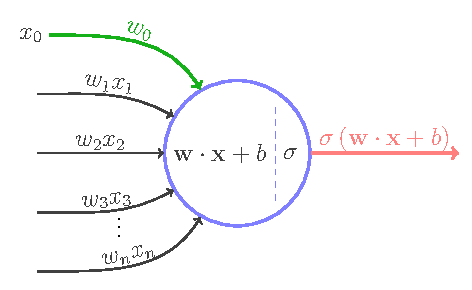
\includegraphics[width=\textwidth]{figures/neuron.pdf}
    \caption{}
    \label{fig:neuron_a}
  \end{subfigure}

  \par\bigskip

  \begin{subfigure}[]{0.5\textwidth}
    \centering
    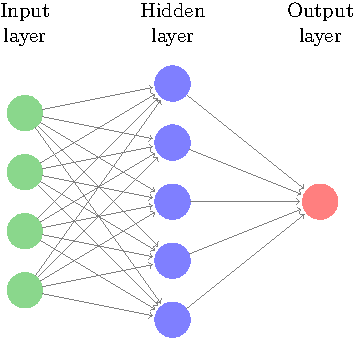
\includegraphics[width=\textwidth]{figures/network.pdf}
    \caption{}
    \label{fig:neuron_b}
  \end{subfigure}
  \caption{
    (a) A mathematical model of a biological neuron.
    (b) A schematic diagram of a neural network with one hidden layer.
    }
\end{figure*}

\begin{figure}
  \centering
  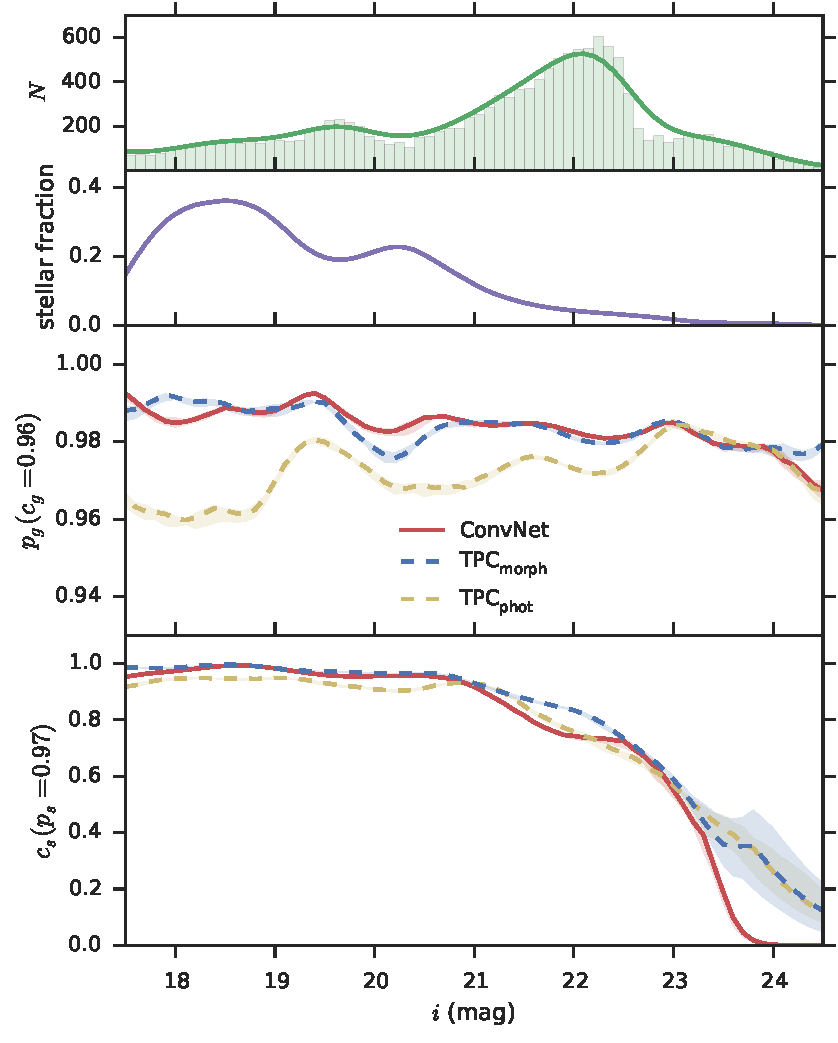
\includegraphics[width=0.7\linewidth]{figures/clens_mag.pdf}
  \caption{Galaxy purity and star completeness values as functions
           of the $i$-band magnitude (differential counts)
           as estimated by kernel density estimation (KDE)
           in the CFHTLenS data set.
           The top panel shows the histogram with a bin size of 0.1 mag
           and the KDE for objects in the test set.
           The second panel shows the fraction of stars estimated by KDE
           as a function of magnitude.
           The bottom two panels compare the galaxy purity and star completeness
           values for ConvNet (red solid line),
           $\mathrm{TPC}_{\mathrm{morph}}$ (blue dashed line),
           and $\mathrm{TPC}_{\mathrm{phot}}$ (yellow dashed line)
           as functions of magnitude.
           The $1 \sigma$ confidence bands are estimated by
           bootstrap sampling.}
  \label{fig:clens_mag}
\end{figure}

\begin{figure}
  \centering
  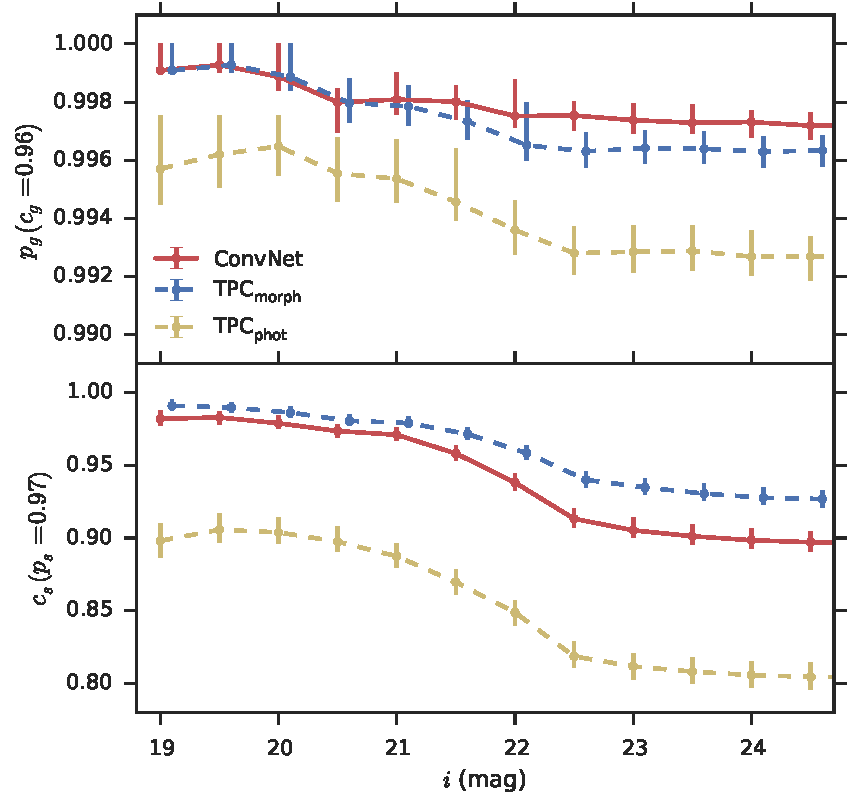
\includegraphics[width=0.7\linewidth]{figures/clens_integrated.pdf}
  \caption{
    Galaxy purity and star completeness as functions of the $i$-band
    magnitude (integrated counts) in the CFHTLenS data set.
    The upper panel compares the galaxy
    purity values for ConvNet (red solid line), $\mathrm{TPC}_{\mathrm{morph}}$
    (blue dashed line), and $\mathrm{TPC}_{\mathrm{phot}}$ (yellow dashed line).
    The lower panel compares the star completeness values.
    The $1 \sigma$ error bars are computed following the method
    of \citet{paterno2004calculating} to avoid the unphysical
    errors of binomial or Poisson statistics.
    }
  \label{fig:clens_integrated}
\end{figure}

\begin{figure}
  \centering
  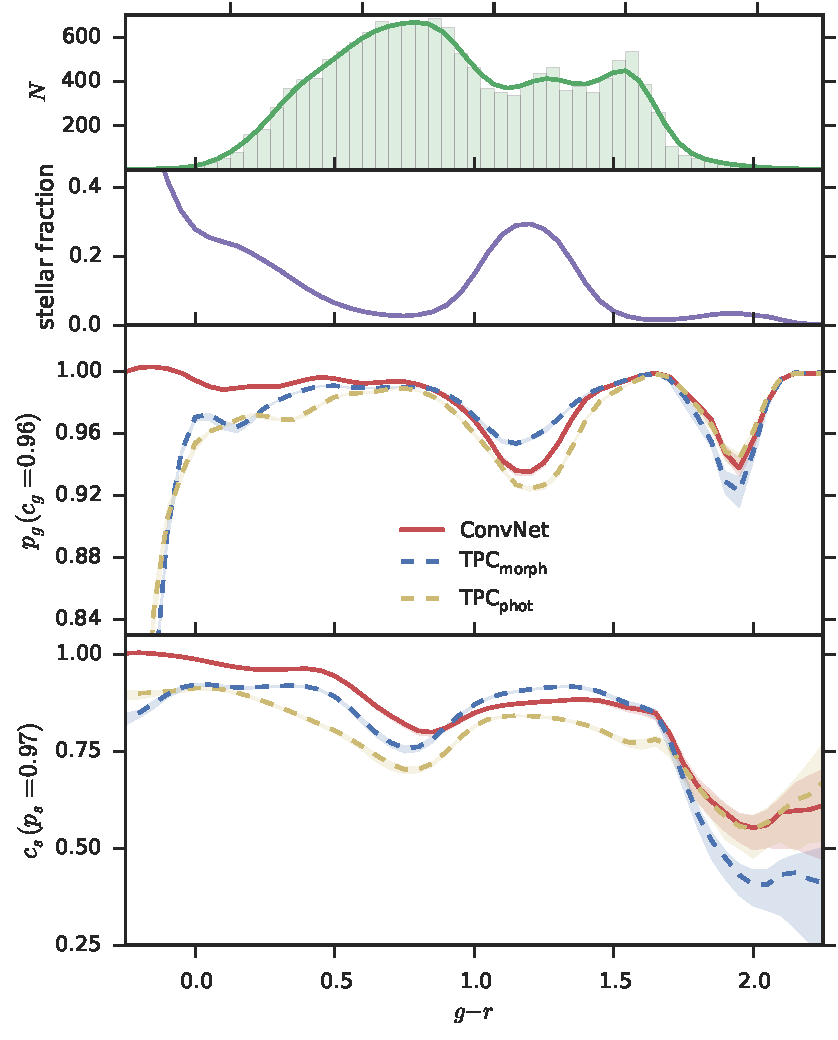
\includegraphics[width=0.7\linewidth]{figures/clens_g_r.pdf}
  \caption{Similar to Figure~\ref{fig:clens_mag}
           but as a function of $g-r$ color.
           The bin size of histogram in the top panel is 0.05.}
  \label{fig:clens_g_r}
\end{figure}

\begin{figure}
  \centering
  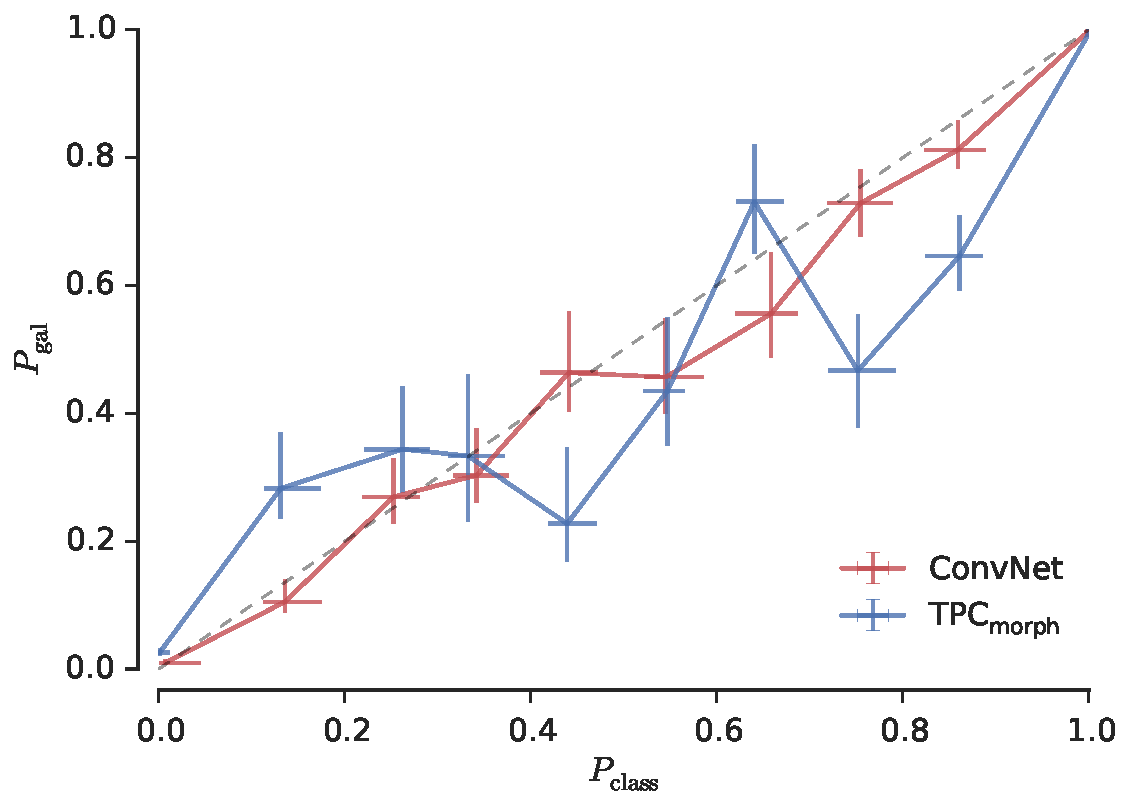
\includegraphics[width=0.7\linewidth]{figures/clens_calibration.pdf}
  \caption{
    The calibration curves for ConvNet (red) and $\mathrm{TPC}_{\mathrm{morph}}$ (blue)
    as applied to the CFHTLenS data set.
    $P_{\mathrm{gal}}$ is the fraction of objects that are galaxies, and
    $P_{\mathrm{class}}$ is the probabilistic outputs generated by the classifiers.
    The dashed line displays the relationship
    $P_{\mathrm{gal}} = P_{\mathrm{conv}}$.
    The $1 \sigma$ error bars are computed following the method
    of \citet{paterno2004calculating}.
    }
  \label{fig:clens_calibration}
\end{figure}

\begin{sidewaysfigure*}
  \centering
  \begin{subfigure}[c]{0.24\linewidth}
  \centering
    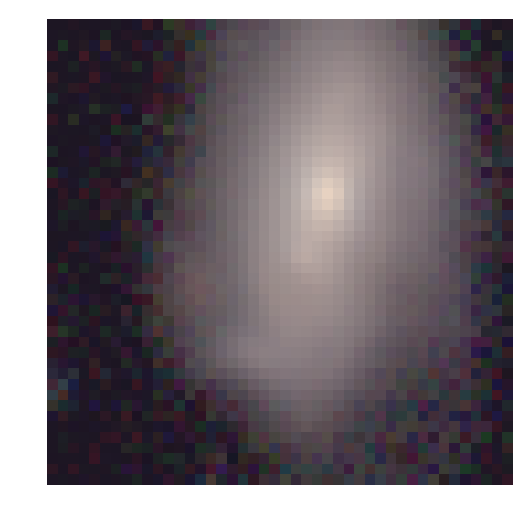
\includegraphics[width=\textwidth]{figures/galaxy_original.pdf}
    \caption{Input (5 bands$\times44\times44$)}
  \end{subfigure}
  \hfill
  \begin{subfigure}[c]{0.24\linewidth}
  \centering
    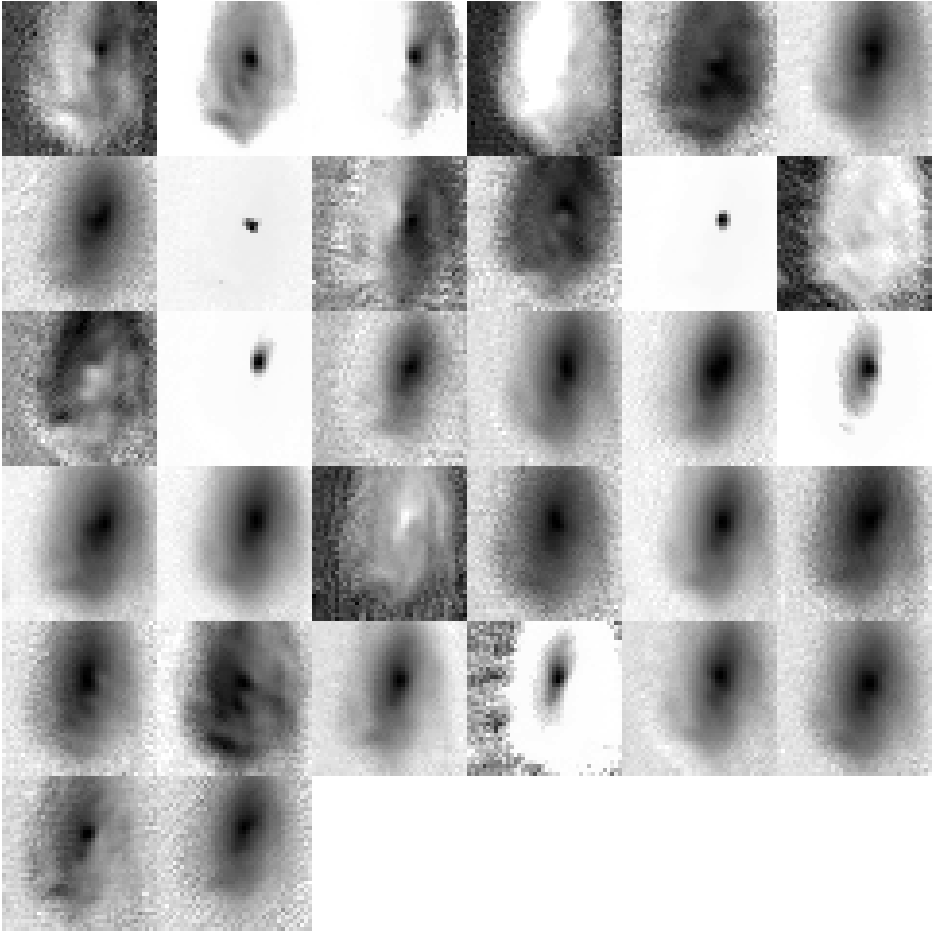
\includegraphics[width=\textwidth]{figures/galaxy_conv11.pdf}
    \caption{Layer 1 (32 maps$\times40\times40$)}
  \end{subfigure}
  \hfill
  \begin{subfigure}[c]{0.24\linewidth}
  \centering
    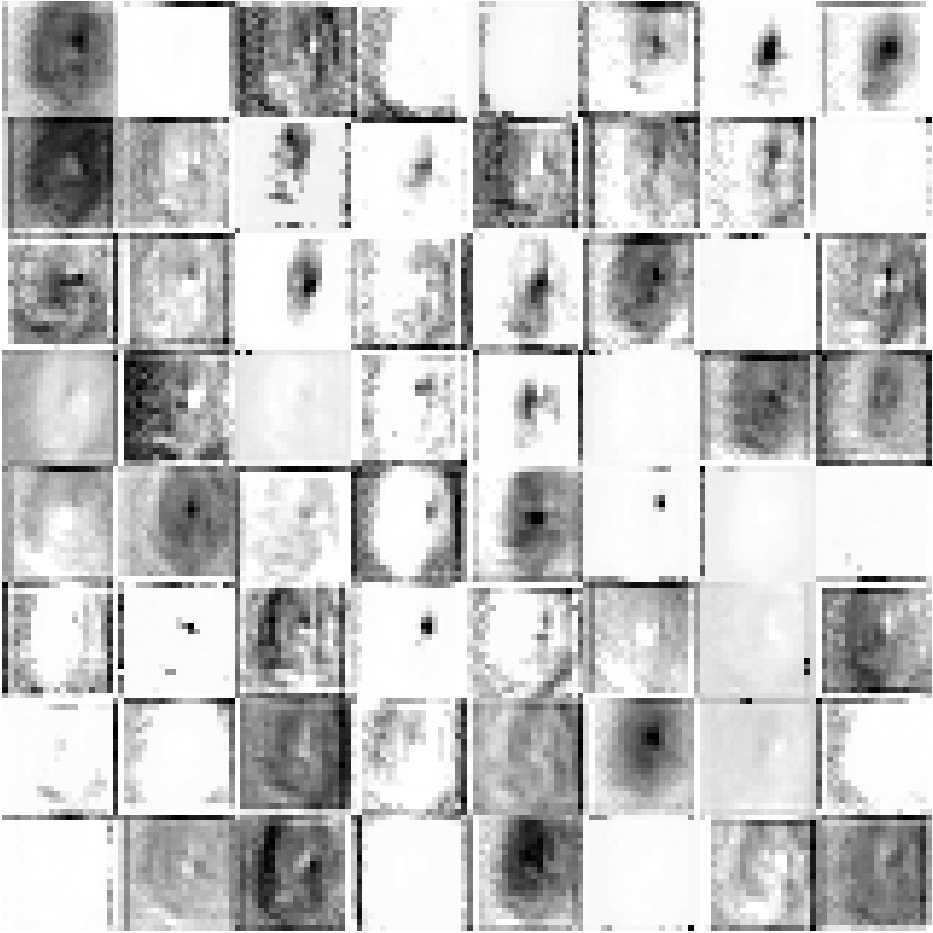
\includegraphics[width=\textwidth]{figures/galaxy_conv21.pdf}
    \caption{Layer 3 (64 maps$\times20\times20$)}
  \end{subfigure}
  \hfill
  \begin{subfigure}[c]{0.24\linewidth}
  \centering
    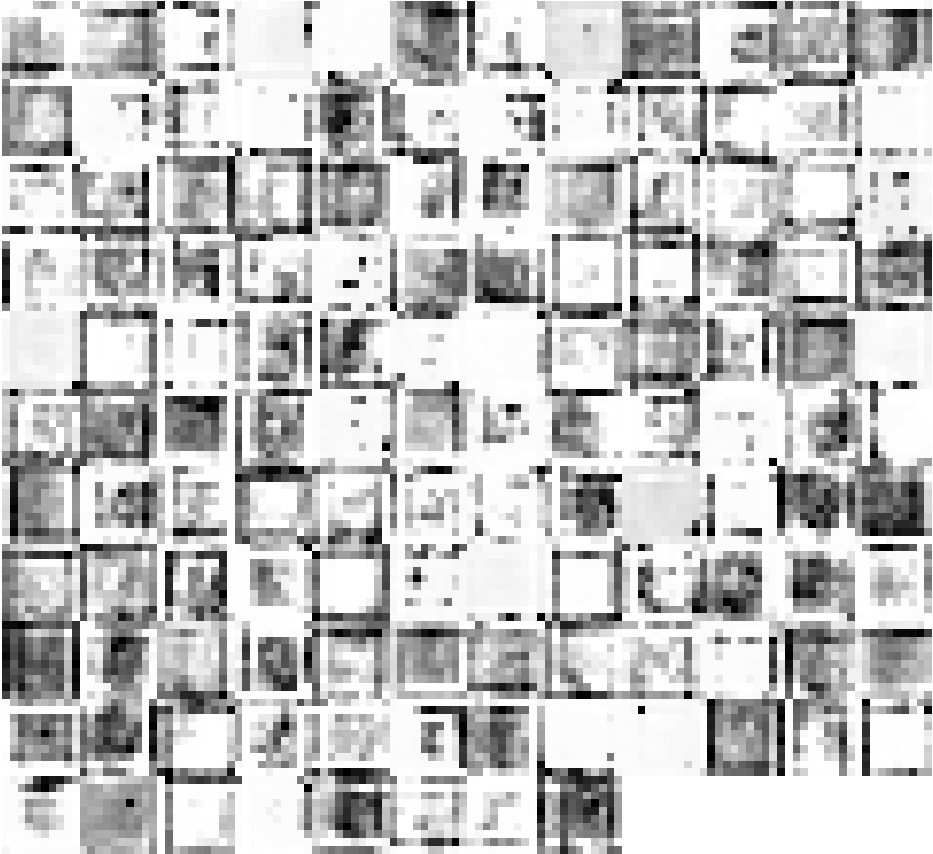
\includegraphics[width=\textwidth]{figures/galaxy_conv31.pdf}
    \caption{Layer 6 (128 maps$\times10\times10$)}
  \end{subfigure}
  \caption{
    (a) A sample $44\times44$ RGB image of a galaxy in the CFHTLenS data set.
    The RGB image is created by mapping R $\rightarrow i$ band magnitude,
    G $\rightarrow r$ band magnitude, and B $\rightarrow g$ band magnitude.
    (b) Activations on the first convolutional layer when a $5\times44\times44$
    image is fed into the network.
    (c) Activations on the third convolutional layer.
    (d) Activations on the sixth convolutional layer.
    Each image in (b), (c), and (d) is a feature map corresponding to the
    output for one of the learned features.
    }
  \label{fig:galaxy_activations}
\end{sidewaysfigure*}


\begin{sidewaysfigure*}
  \centering
  \begin{subfigure}[c]{0.24\linewidth}
  \centering
    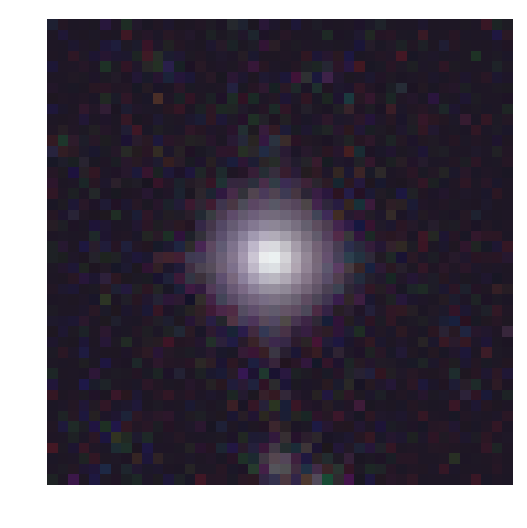
\includegraphics[width=\textwidth]{figures/star_original.pdf}
    \caption{Input (5 bands$\times44\times44$)}
  \end{subfigure}
  \hfill
  \begin{subfigure}[c]{0.24\linewidth}
  \centering
    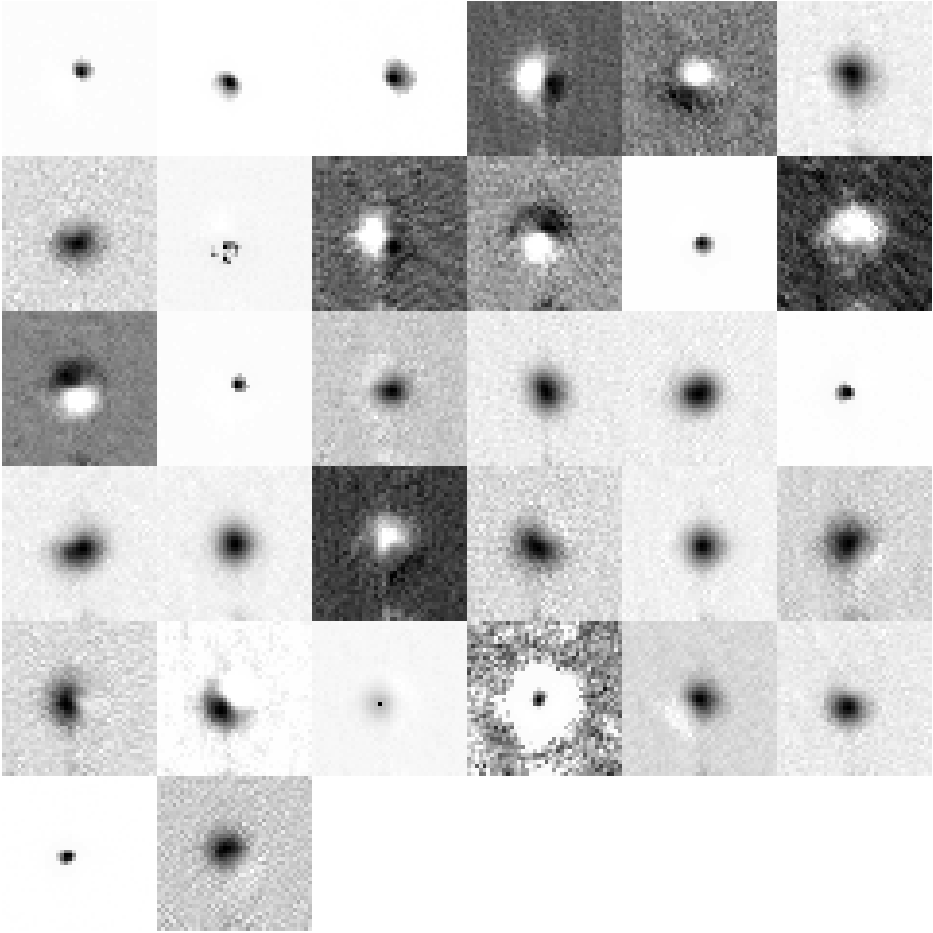
\includegraphics[width=\textwidth]{figures/star_conv11.pdf}
    \caption{Layer 1 (32 maps$\times40\times40$)}
  \end{subfigure}
  \hfill
  \begin{subfigure}[c]{0.24\linewidth}
  \centering
    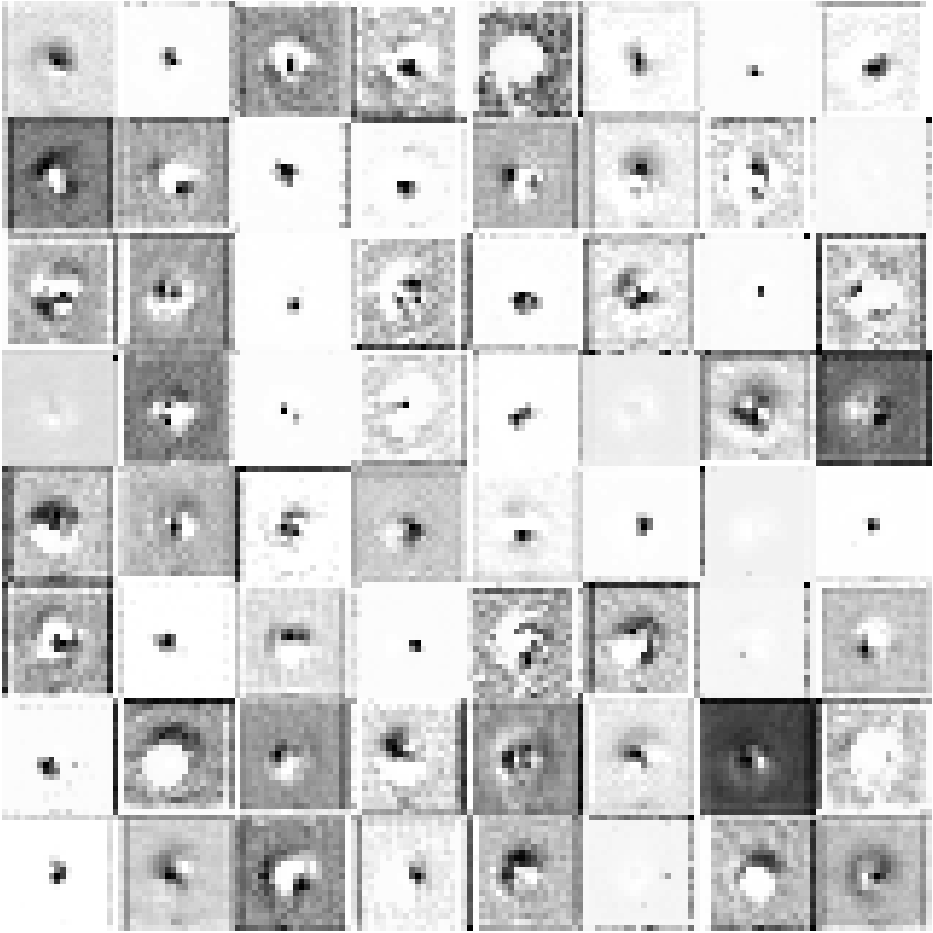
\includegraphics[width=\textwidth]{figures/star_conv21.pdf}
    \caption{Layer 3 (64 maps$\times20\times20$)}
  \end{subfigure}
  \hfill
  \begin{subfigure}[c]{0.24\linewidth}
  \centering
    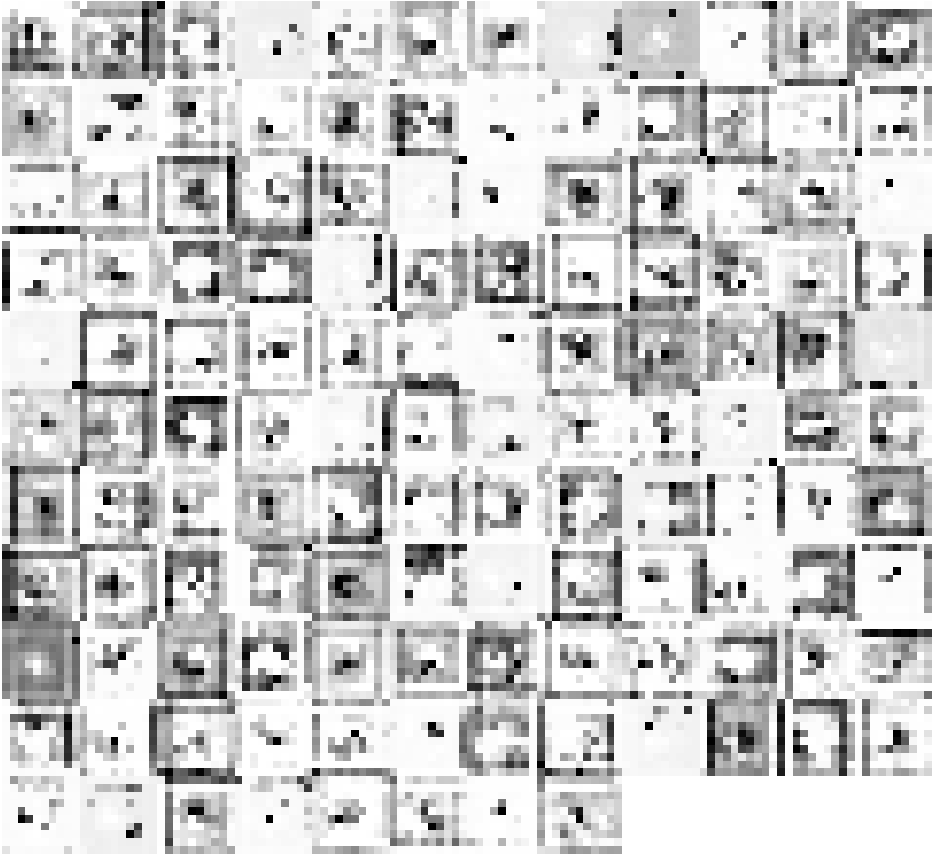
\includegraphics[width=\textwidth]{figures/star_conv31.pdf}
    \caption{Layer 6 (128 maps$\times10\times10$)}
  \end{subfigure}
  \caption{
    Similar to Figure~\ref{fig:galaxy_activations} but for a star in the
    CFHTLenS data set.
    }
  \label{fig:star_activations}
\end{sidewaysfigure*}

\begin{figure}
  \centering
  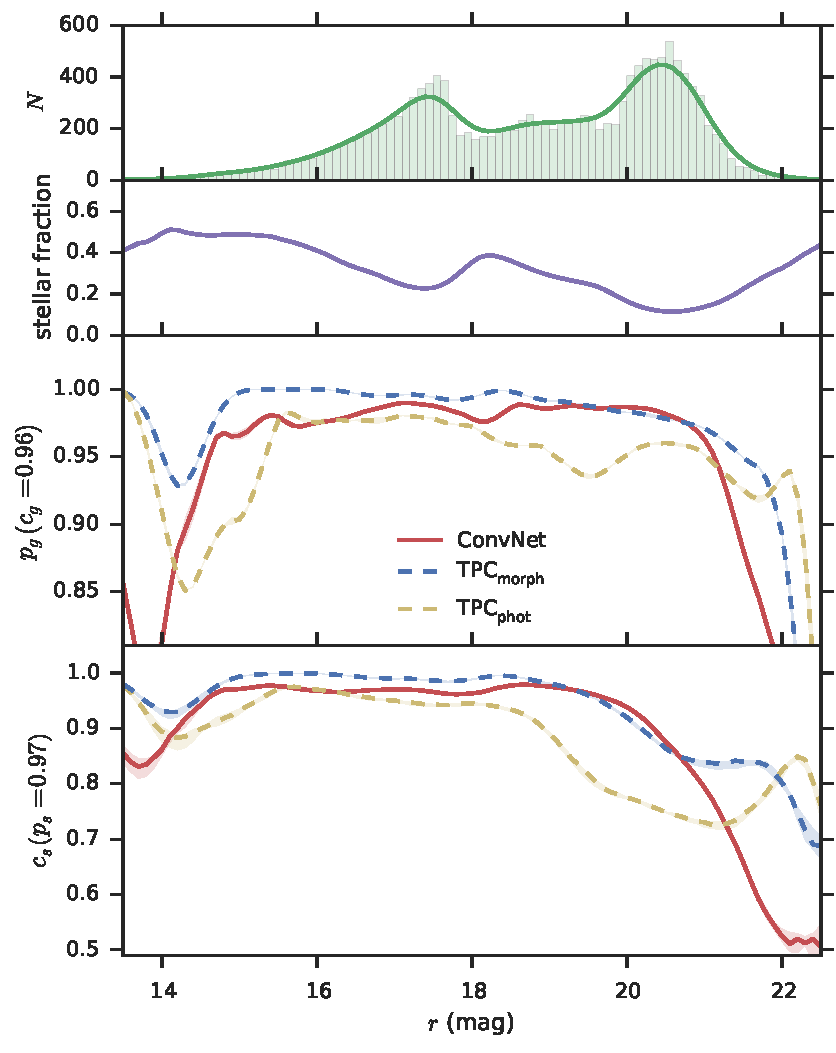
\includegraphics[width=0.7\linewidth]{figures/sdss_mag.pdf}
  \caption{Galaxy purity and star completeness as function of the $r$-band
    magnitude for the differential counts in the SDSS data set.}
  \label{fig:sdss_mag}
\end{figure}

\begin{figure}
  \centering
  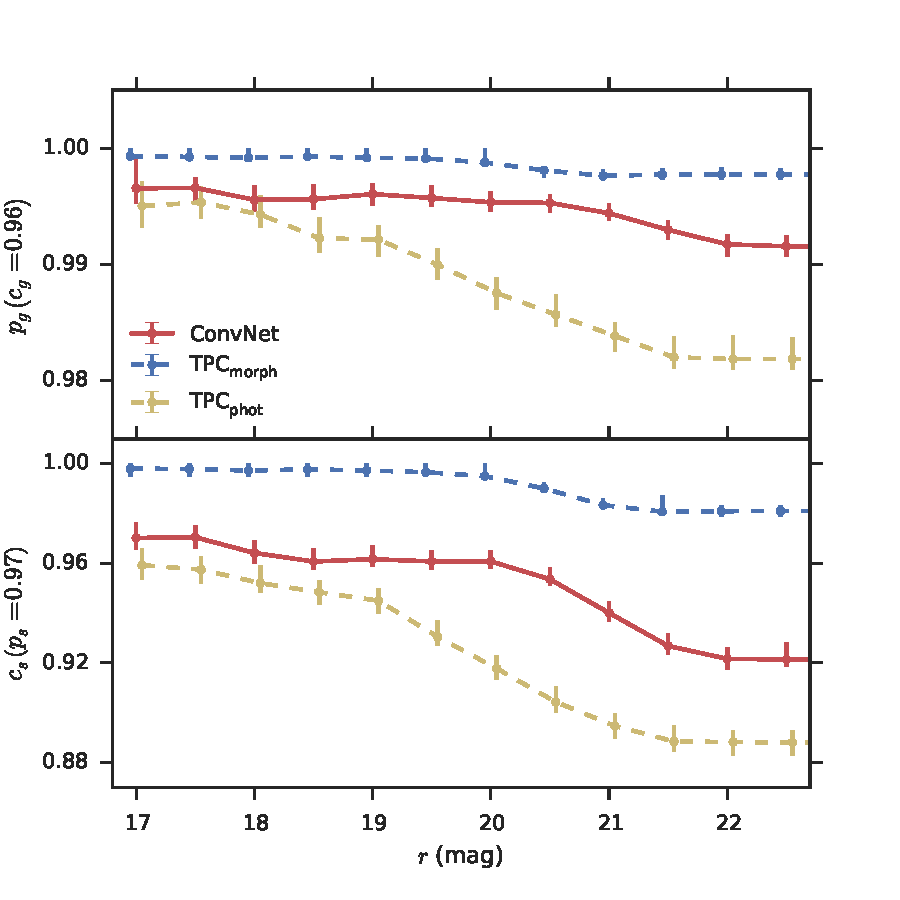
\includegraphics[width=0.7\linewidth]{figures/sdss_integrated.pdf}
  \caption{Galaxy purity and star completeness as functions of the $r$-band
    magnitude for the integrated counts in the SDSS data set.}
  \label{fig:sdss_integrated}
\end{figure}

\begin{figure}
  \centering
  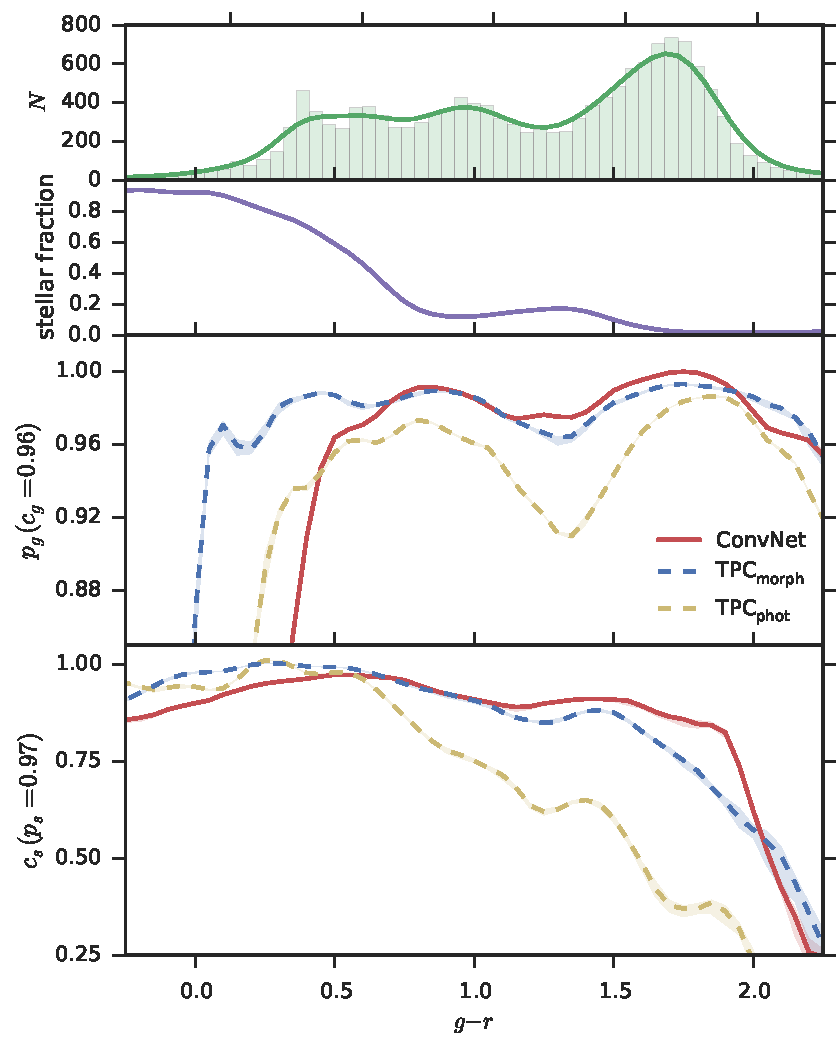
\includegraphics[width=0.7\linewidth]{figures/sdss_g_r.pdf}
  \caption{Similar to Figure~\ref{fig:sdss_mag} but as a function of
    $g-r$ color. The bin size of histogram in the top panel is 0.05.}
  \label{fig:sdss_g_r}
\end{figure}

\begin{figure}
  \centering
  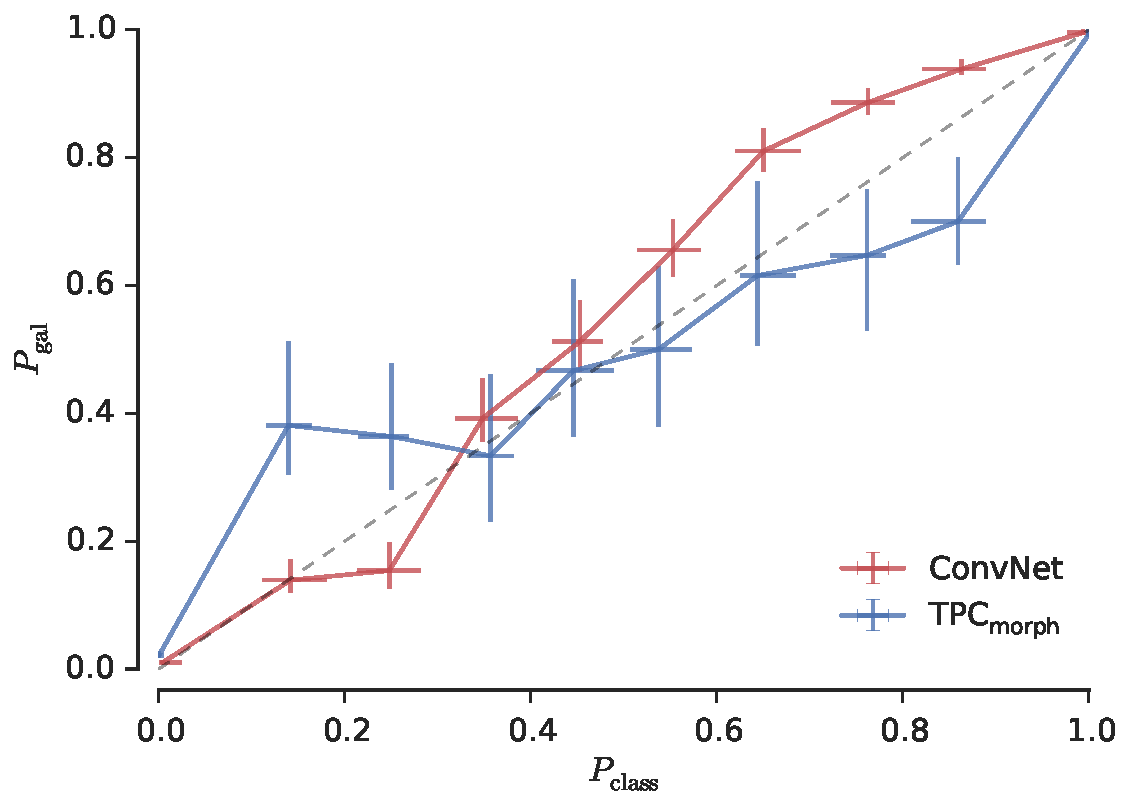
\includegraphics[width=0.7\linewidth]{figures/sdss_calibration.pdf}
  \caption{
    Calibration curves for ConvNet (red) and $\mathrm{TPC}_{\mathrm{morph}}$
    (blue) as applied to the SDSS data set.
    }
  \label{fig:sdss_calibration}
\end{figure}

\begin{sidewaysfigure*}
  \centering
  \begin{subfigure}[c]{0.24\linewidth}
  \centering
    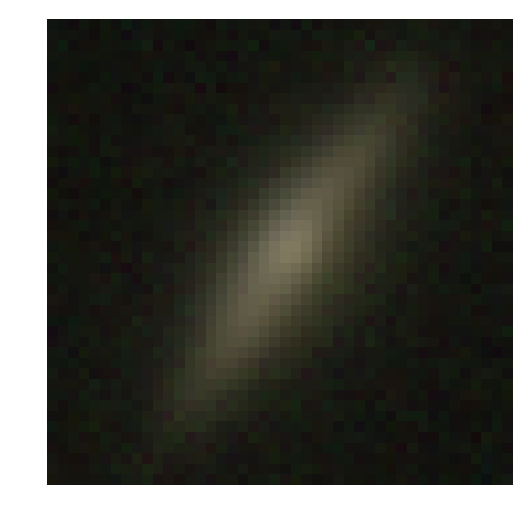
\includegraphics[width=\textwidth]{figures/sdss_galaxy_original.pdf}
    \caption{Input (5 bands$\times44\times44$)}
  \end{subfigure}
  \hfill
  \begin{subfigure}[c]{0.24\linewidth}
  \centering
    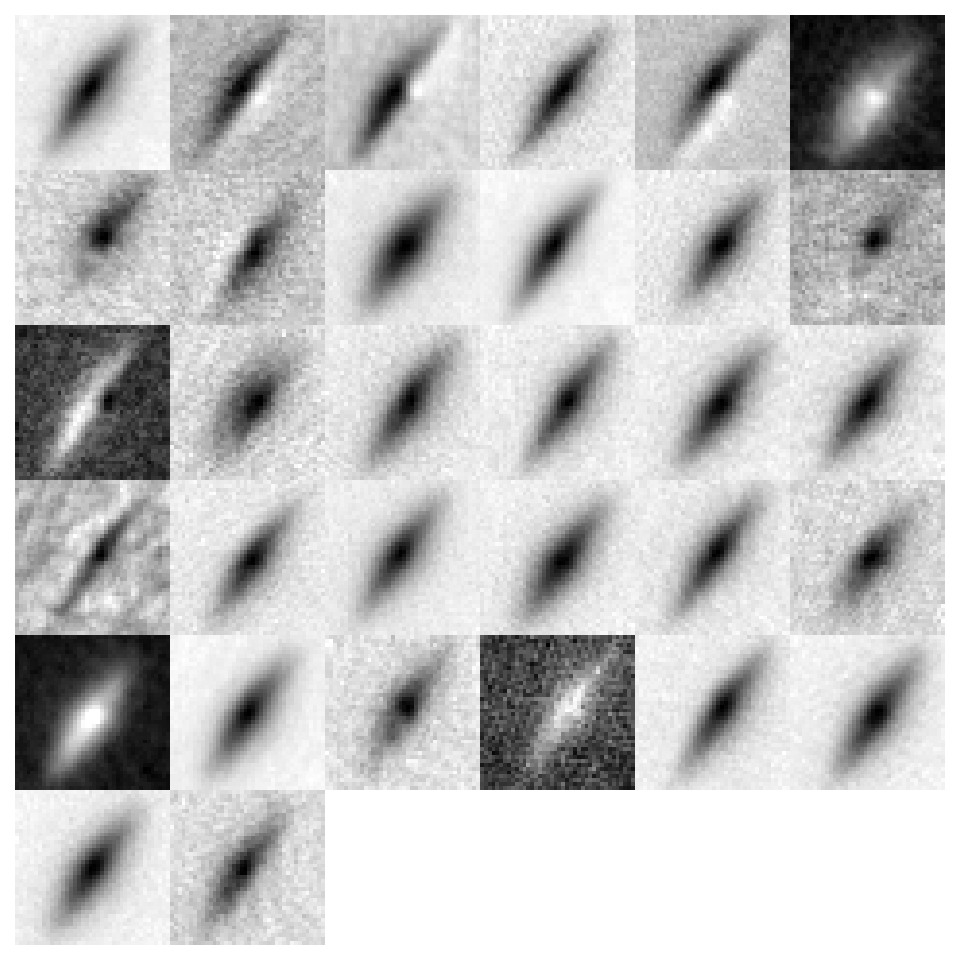
\includegraphics[width=\textwidth]{figures/sdss_galaxy_conv11.pdf}
    \caption{Layer 1 (32 maps$\times40\times40$)}
  \end{subfigure}
  \hfill
  \begin{subfigure}[c]{0.24\linewidth}
  \centering
    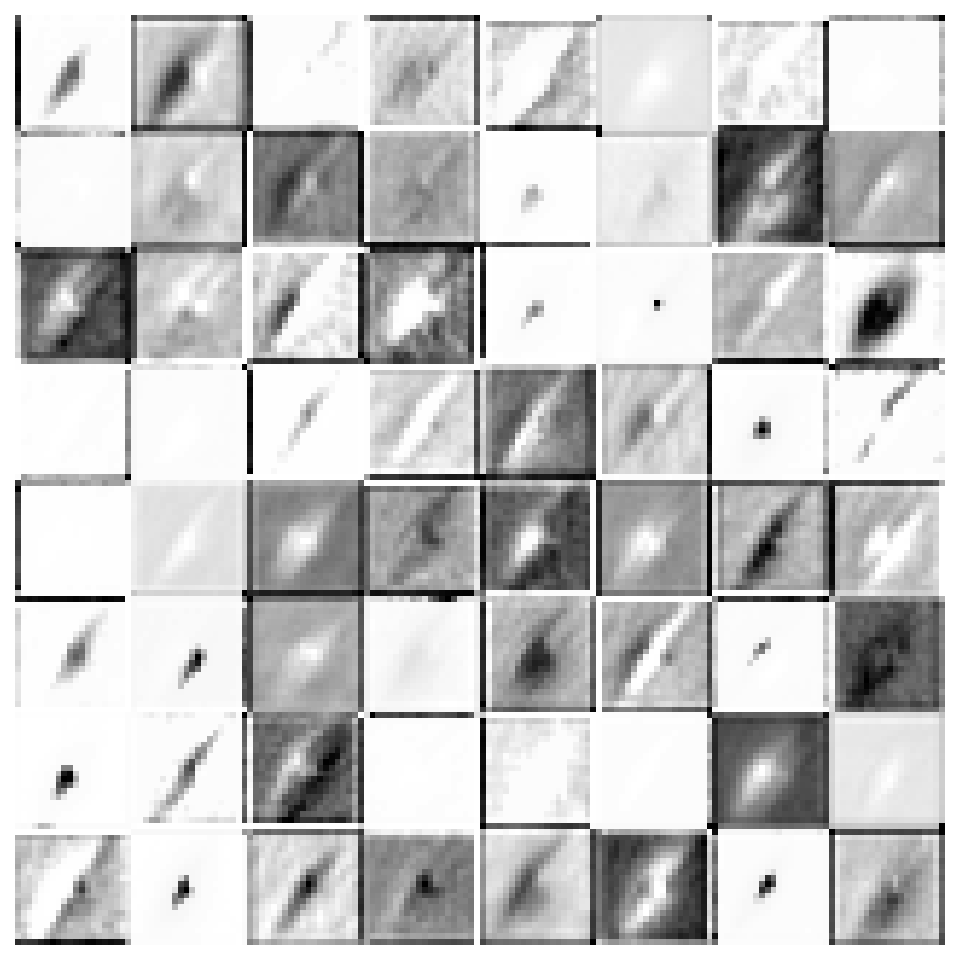
\includegraphics[width=\textwidth]{figures/sdss_galaxy_conv21.pdf}
    \caption{Layer 3 (64 maps$\times20\times20$)}
  \end{subfigure}
  \hfill
  \begin{subfigure}[c]{0.24\linewidth}
  \centering
    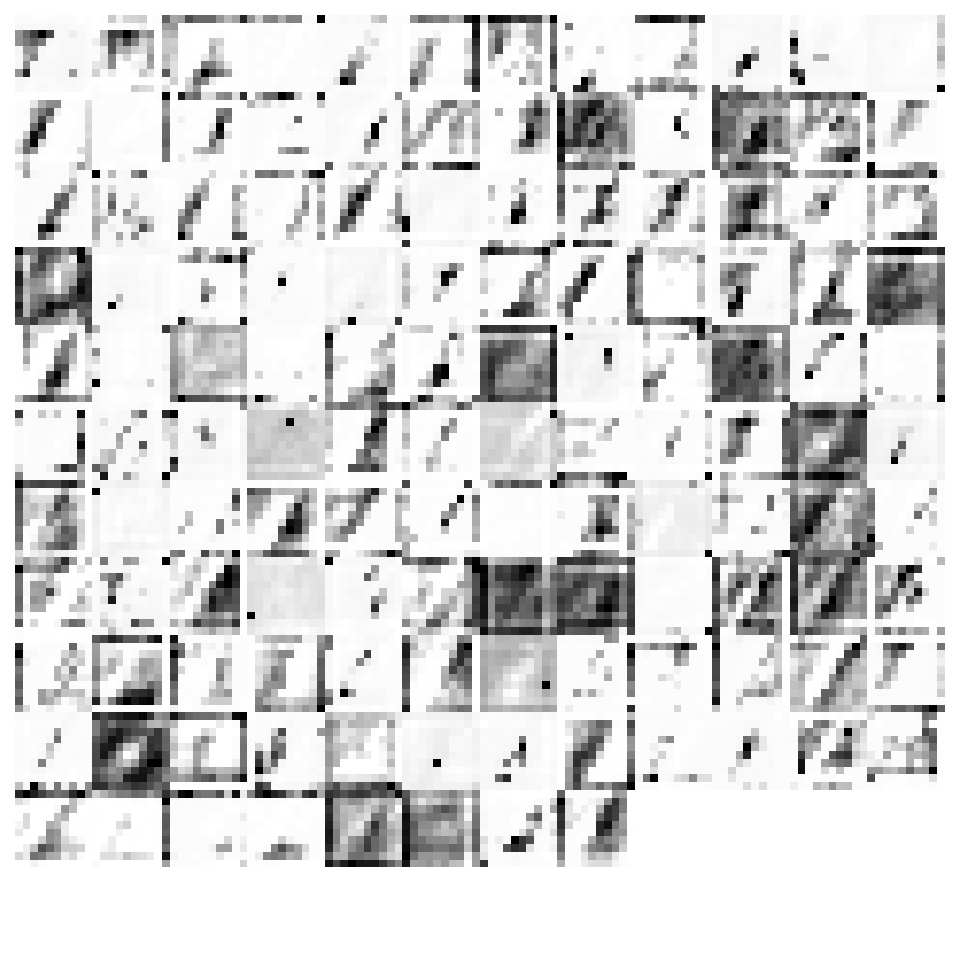
\includegraphics[width=\textwidth]{figures/sdss_galaxy_conv31.pdf}
    \caption{Layer 6 (128 maps$\times10\times10$)}
  \end{subfigure}
  \caption{
    Similar to Figure~\ref{fig:galaxy_activations} but for a galaxy in the
    SDSS data set.
    }
  \label{fig:sdss_galaxy_activations}
\end{sidewaysfigure*}

\begin{sidewaysfigure*}
  \centering
  \begin{subfigure}[c]{0.24\linewidth}
  \centering
    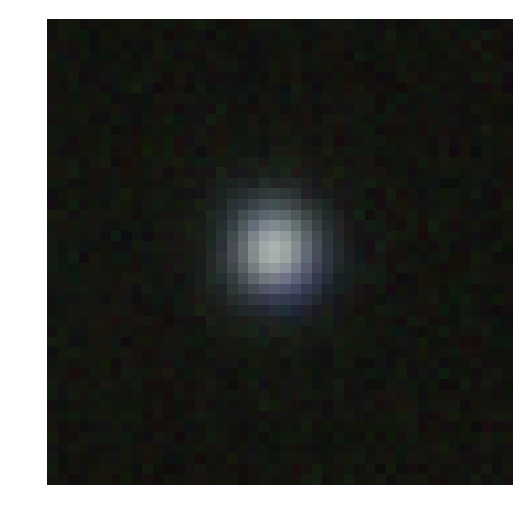
\includegraphics[width=\textwidth]{figures/sdss_star_original.pdf}
    \caption{Input (5 bands$\times44\times44$)}
  \end{subfigure}
  \hfill
  \begin{subfigure}[c]{0.24\linewidth}
  \centering
    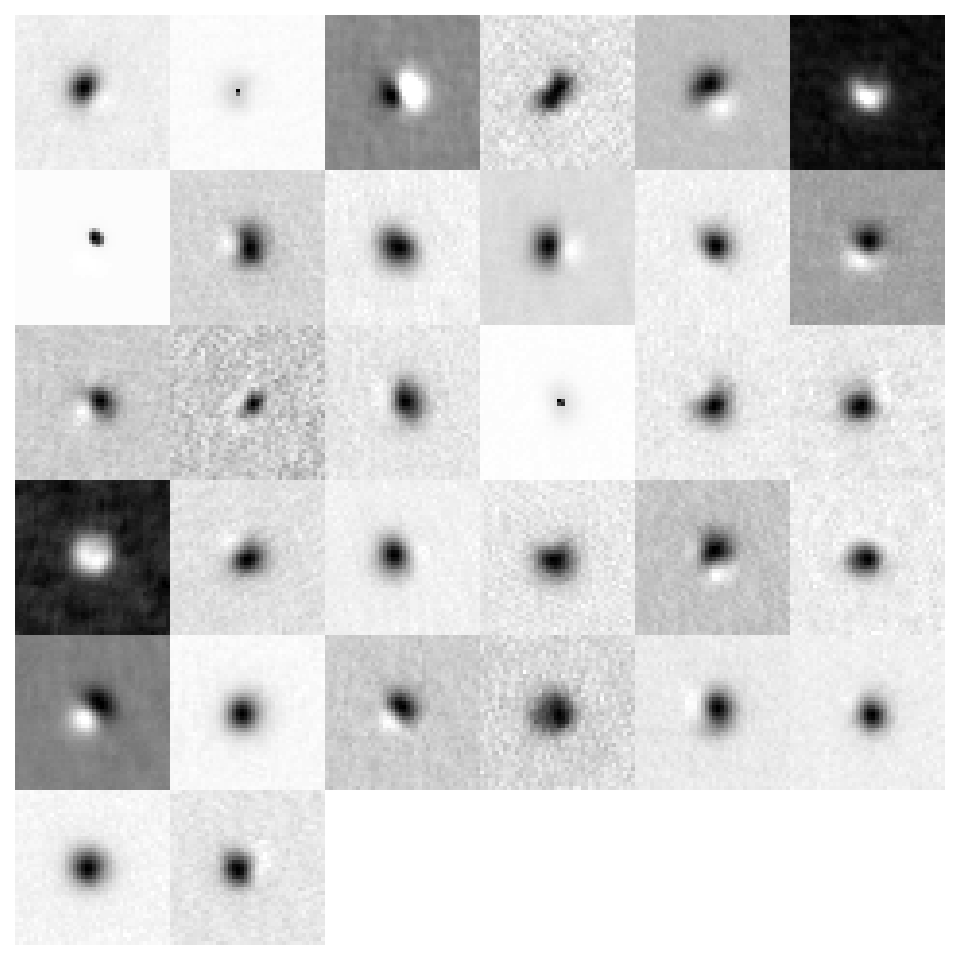
\includegraphics[width=\textwidth]{figures/sdss_star_conv11.pdf}
    \caption{Layer 1 (32 maps$\times40\times40$)}
  \end{subfigure}
  \hfill
  \begin{subfigure}[c]{0.24\linewidth}
  \centering
    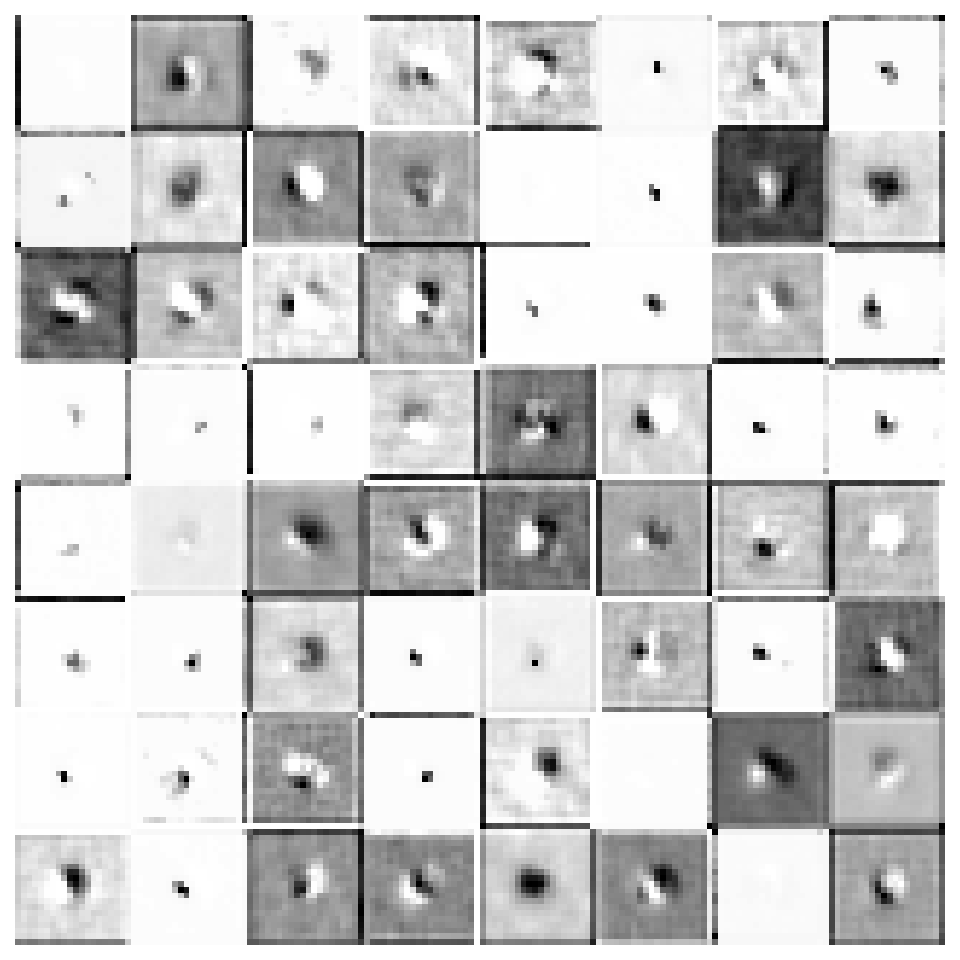
\includegraphics[width=\textwidth]{figures/sdss_star_conv21.pdf}
    \caption{Layer 3 (64 maps$\times20\times20$)}
  \end{subfigure}
  \hfill
  \begin{subfigure}[c]{0.24\linewidth}
  \centering
    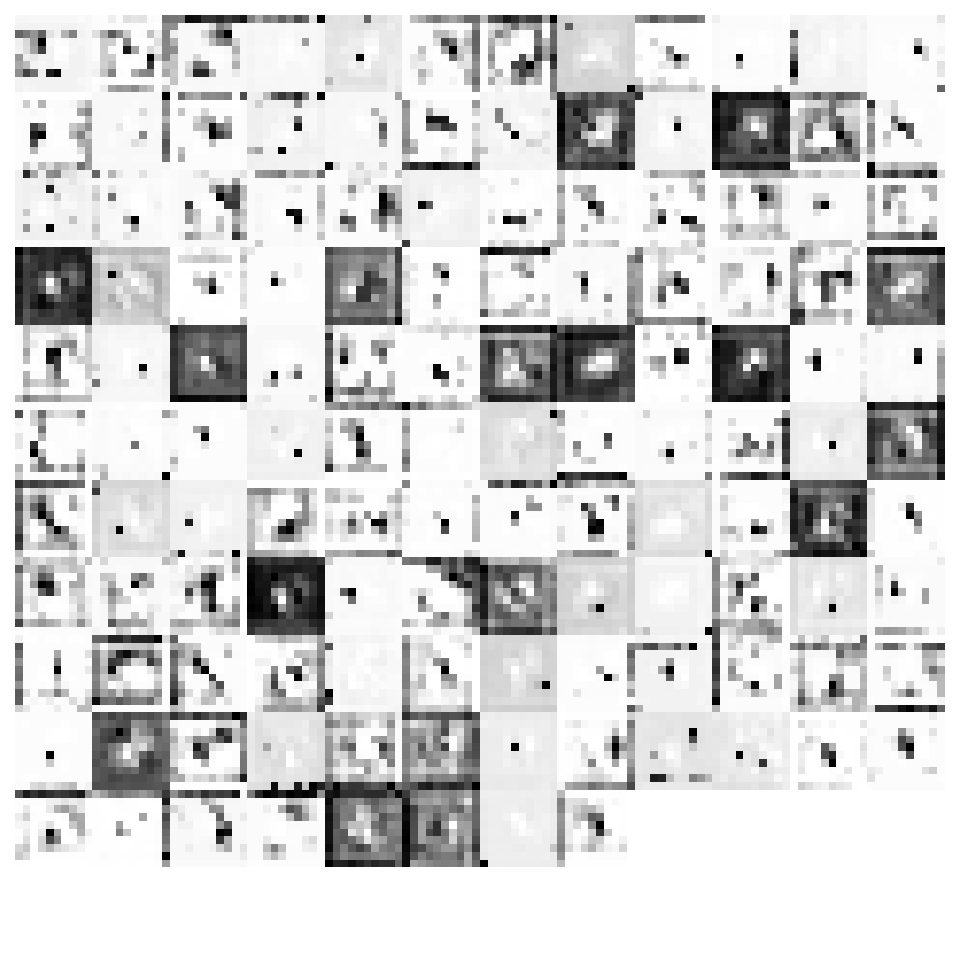
\includegraphics[width=\textwidth]{figures/sdss_star_conv31.pdf}
    \caption{Layer 6 (128 maps$\times10\times10$)}
  \end{subfigure}
  \caption{
    Similar to Figure~\ref{fig:sdss_galaxy_activations} but for a star in the
    SDSS data set.
    }
  \label{fig:sdss_star_activations}
\end{sidewaysfigure*}

\clearpage
\begin{sidewaystable*}
  \centering
  \caption{Summary of ConvNet architecture and hyperparameters. Note that pooling layers have no learnable parameters.}
  \label{table:hyperparamters}
  \begin{tabular}{ccccccc}
    \hline
    type            & filters & filter size & padding & non-linearity & initial weights & initial biases \\
    \hline
    convolutional   & 32          & $5\times5$  & -       & leaky ReLU    & orthogonal      & 0.1            \\
    convolutional   & 32          & $3\times3$  & 1       & leaky ReLU    & orthogonal      & 0.1            \\
    pooling         & -           & $2\times2$  & -       & -             & -               & -              \\
    convolutional   & 64          & $3\times3$  & 1       & leaky ReLU    & orthogonal      & 0.1            \\
    convolutional   & 64          & $3\times3$  & 1       & leaky ReLU    & orthogonal      & 0.1            \\
    convolutional   & 64          & $3\times3$  & 1       & leaky ReLU    & orthogonal      & 0.1            \\
    pooling         & -           & $2\times2$  & -       & -             & -               & -              \\
    convolutional   & 128         & $3\times3$  & 1       & leaky ReLU    & orthogonal      & 0.1            \\
    convolutional   & 128         & $3\times3$  & 1       & leaky ReLU    & orthogonal      & 0.1            \\
    convolutional   & 128         & $3\times3$  & 1       & leaky ReLU    & orthogonal      & 0.1            \\
    pooling         & -           & $2\times2$  & -       & -             & -               & -              \\
    fully-connected & 2048        & -           & -       & leaky ReLU    & orthogonal      & 0.01            \\
    fully-connected & 2048        & -           & -       & leaky ReLU    & orthogonal      & 0.01            \\
    fully-connected & 2           & -           & -       & softmax       & orthogonal      & 0.01            \\
    \hline
  \end{tabular}
\end{sidewaystable*}

\begin{table}
  \caption{The definition of the classification performance metrics.}
  \centering
  \begin{tabular}{c l}
  \hline
  Metric & Meaning \\
  \hline
  AUC & Area under the Receiver Operating Curve \\
  MSE & Mean squared error \\
  $c_g$ & Galaxy completeness \\
  $p_g$ & Galaxy purity \\
  $c_s$ & Star completeness \\
  $p_s$ & Star purity \\
  $p_g(c_g=x)$ & Galaxy purity at $x$ galaxy completeness \\
  $c_s(p_s=x)$ & Star completeness at $x$ star purity \\
  $CAL$ & Calibration error with overlapping binning \\
  $\mid\Delta N_g\mid / N_g$ & Absolute error in number of galaxies\\
log loss
&
Cross-entropy
\\
  \hline
  \end{tabular}
  \label{table:metrics}
\end{table}

\begin{sidewaystable*}
  \caption{
    A summary of the classification performance metrics
    as applied to the CFHTLenS data.
    The definition of the metrics is summarized in Table~\ref{table:metrics}.
    The bold entries highlight the best performance values within each column.
    Note that $p_{g}(c_g=0.96)$ and $c_{s}(p_s=0.97)$ require adjusting
    threshold values (\ie probability cuts), while other metrics do not.
    To obtain a galaxy completeness of $c_g=0.96$, we choose the threshold values
    0.9972, 0.9963, and 0.9927 for ConvNet, TPC${}_{\mathrm{morph}}$, and 
    TPC${}_{\mathrm{phot}}$, respectively;
    for star purity $p_s=0.97$, we choose 0.6990, 0.5297, and 0.8570 for
    ConvNet, TPC${}_{\mathrm{morph}}$, and TPC${}_{\mathrm{phot}}$, respectively.
  }
  \centering
  \begin{tabular}{l c c c c c c c}
    \hline
    classifier & AUC & MSE & $p_{g}(c_g=0.96)$ & $c_{s}(p_s=0.97)$ & CAL & $ |\Delta N_g|/N_g$ &
log loss
\\
    \hline
    ConvNet                       & \textbf{0.9948} & 0.0112          & \textbf{0.9972} & 0.8971          & \textbf{0.0197}  & \textbf{0.0029} &
\textbf{0.0441}
\\
    TPC${}_{\mathrm{morph}}$         & 0.9924          & \textbf{0.0109} & 0.9963          & \textbf{0.9268} & 0.0245           & 0.0056 &
0.0809
\\
    TPC${}_{\mathrm{phot}}$          & 0.9876          & 0.0189          & 0.9927          & 0.8044          & 0.0266           & 0.0101 &
0.1085
\\
    \hline
  \end{tabular}
  \label{table:clens_metrics}
\end{sidewaystable*}

\begin{sidewaystable*}
  \caption{
    A summary of the classification performance metrics
    as applied to the SDSS data.
    To obtain a galaxy completeness of $c_g=0.96$, we choose the threshold values
    0.7558, 0.9989, and 0.9360 for ConvNet, TPC${}_{\mathrm{morph}}$, and
    TPC${}_{\mathrm{phot}}$, respectively;
    for star purity $p_s=0.97$, we choose 0.6046, 0.0547, and 0.7449 for
    ConvNet, TPC${}_{\mathrm{morph}}$, and TPC${}_{\mathrm{phot}}$, respectively.
  }
  \centering
  \begin{tabular}{l c c c c c c c}
    \hline
    classifier & AUC & MSE & $p_{g}(c_g=0.96) $ & $c_{s}(p_s=0.97)$ & CAL & $ |\Delta N_g|/N_g$ &
log loss
\\
    \hline
    ConvNet               & 0.9952          & 0.0182          & 0.9915          & 0.9500          & \textbf{0.0243} & 0.0157 &
\textbf{0.0731}
\\
    TPC${}_{\mathrm{morph}}$ & \textbf{0.9967} & \textbf{0.0099} & \textbf{0.9977} & \textbf{0.9810} & 0.0254          & \textbf{0.0044} & 
0.0914
\\
    TPC${}_{\mathrm{phot}}$  & 0.9886          & 0.0283          & 0.9819          & 0.8879          & 0.0316          & 0.0160 & 
0.1372
\\
    \hline
  \end{tabular}
  \label{table:sdss_metrics}
\end{sidewaystable*}


\clearpage
\bibliographystyle{plainnat}
\bibliography{thesisbib}
\chapter{Star-galaxy Classification Using Semi-Supervised Generative Adversarial Networks}
  \label{chapter4}

\blfootnote{
This chapter contains material from the following previously published article:
\nobibliography{thesisbib}
\begin{itemize}
\item\bibentry{kim2018star}
\end{itemize}
}

% Introduction
\section{Introduction}
  \label{sec:introduction}

The Sloan Digital Sky Survey \citep[SDSS;][]{york2000sloan}, one of the most successful surveys to date,
has obtained photometric observations of more than $3 \times 10^8$ objects, covering more than one-third of
the sky.
The SDSS has also conducted spectroscopic follow-up observations of more than $3 \times 10^6$
objects \citep{eisenstein2011sdss}.
However, the spectroscopic sample is about one hundred times smaller than the photometric sample,
since spectroscopy is considerably more expensive than photometry in terms of telescope time.
Due to the difficulty of making spectroscopic measurements,
modern, large-scale surveys, such as the Dark Energy Survey (DES),
and the Large Synoptic Survey Telescope (LSST), are purely photometric surveys.
The scarcity of spectroscopic samples will only be exacerbated in the current and next generation of surveys,
as they probe larger cosmological volumes and the majority of photometric observations become too faint
for a uniform spectroscopic follow-up.

Machine learning techniques have been a popular method for classifying stars and galaxies in large sky surveys.
\citet{odewahn1992automated} pioneered the use of artificial neural networks in star-galaxy classification.
Some of the more recent examples of applying machine learning techniques to the star-galaxy classification problem include
decision trees \citep[\eg][]{ball2006robust},
support vector machines \citep[\eg][]{fadely2012},
and convolutional neural networks \citep{kim2017star}.
All of these techniques are \emph{supervised} learning algorithms,
where the input attributes (\eg magnitudes or colors) are provided along with the truth labels (\eg star or galaxy).
We must be careful when extrapolating these supervised algorithms beyond the limits of the labeled data,
because most machine learning methods commonly assume that the labeled samples are governed by
the same or similar underlying data distribution as the target distribution where we apply our model to make predictions.

\emph{Semi-supervised learning} falls between supervised learning, where training data are completely labeled,
and unsupervised learning, where all training data are unlabeled.
Semi-supervised techniques make use of a large amount of unlabeled data, in conjunction with a small amount of labeled data,
to better capture the underlying data distribution.
Semi-supervised learning is of great interest because there will be many orders of magnitude
more unlabeled than labeled data available in future ground-based imaging surveys.

Generative adversarial networks (GANs) --- a class of state-of-the-art deep learning algorithms commonly used in
image-to-image translation applications --- are usually unsupervised,
but semi-supervised learning variants of GANs have recently been introduced
\citep{springenberg2016unsupervised,salimans2016improved,odena2016semi}.
Unsupervised GANs have previously been applied to several astronomical applications,
but the main focus in these studies is image generation.
For example, using the COSMOS data, \citet{ravanbakhsh2017enabling} trained
Variational Autoencoders---another commonly used generative model---and GANs
to generate new galaxy images with the goal of synthesizing calibration sets for weak gravitational lensing.
\citet{mustafa2017creating} applied a GAN model to the problem of generating cosmological weak lensing convergence maps.
\citet{schawinski2017generative} showed that GANs are able to recover detailed features such as galaxy morphology
from artificially degraded images of low-redshift galaxies.

In this chapter, we study the application of GANs in generating realistic images of not only galaxies,
but also the stars and quasi-stellar objects (QSOs or quasars) in ground-based photometric surveys.
More importantly, we demonstrate that semi-supervised GANs are able to produce accurate and well-calibrated classifications
using only a small number of labeled examples.
The rest of the chapter is organized as follows.
In Section \ref{sec:data}, we describe the SDSS data set and the image pre-processing steps.
In Section \ref{sec:methods}, we provide a brief overview of semi-supervised GANs.
In Section \ref{sec:results}, we present the main results of image generation and source classification using our semi-supervised GAN model.
Finally, we outline our conclusions in Section \ref{sec:conclusions}.

% Data
\section{Data}
  \label{sec:data}
  
  
To demonstrate the performance of our approach, we follow a similar approach to Chapter \ref{chapter3}.
However, we restrict our analysis to data from the SDSS survey in this chapter.
We use SDSS because of the the large number of objects and the concurrent spectroscopy.
In this section, we briefly describe the SDSS data set and the image pre-processing steps for
preparing training examples.

The SDSS survey, one of the largest astronomical surveys that has ever existed,
covers 14,555 square degrees in five bands: $u$, $g$, $r$, $i$, and $z$.
The twelfth data release \citep{alam2015eleventh}, the final data release from SDSS phases I--III,
contains photometry of over $3 \times 10^8$ objects with a limiting magnitude of $r \approx 22$.
More than $3 \times 10^6$ objects from the photometric catalog were also targeted for spectroscopy \citep{eisenstein2011sdss}.

In a semi-supervised learning setting, we typically have a large amount of unlabeled data
and a small amount of labeled data.
Thus, the data sets we use in this work consists of an \emph{unlabeled} training set,
a \emph{labeled} training set, and a blind, \emph{labeled} test set.
For the unlabeled training set, we use the \texttt{photoObj} view of the publicly available CasJobs server \footnote{\url{http://skyserver.sdss.org/casjobs/}} \citep{li2008casjobs},
and randomly select $1 \times 10^6$ objects.
We exclude objects with bad photometric observations as follows.
We only include objects with magnitudes between 0 and 40;
we consider only objects with the half-light radius (as measured by the exponential and de Vaucouleurs light profiles)
in the $r$ band less than 30 arc seconds;
we also exclude any objects with warning flags in the photometric measurement;
and we exclude any images with missing or masked values.
After using the CasJobs server to select objects with clean photometry,
we download the FITS images for SDSS fields covering these objects.
Using the astrometry information in the FITS headers and the \texttt{Montage} \footnote{\url{http://montage.ipac.caltech.edu/}} software,
we align each image in $u$, $g$, $i$, and $z$ bands to the $r$-band image.
To generate cutout images of size $32 \times 32$ pixels that can be used as input to our GAN framework,
we use \texttt{SExtractor} to center each object in the cutout image.
Furthermore, we convert all flux values in the FITS files to luptitudes
\citep[\ie inverse hyperbolic sine magnitudes;][]{lupton1999modified}.
Finally, we use the dust reddening map of \citet{schlegel1998maps} to account for extinction.
Sample postage stamps of typical galaxies, stars, and quasars are shown in Figure \ref{fig:sdss_stamps}.

The labeled training set and the test set are drawn from objects in the \texttt{specObj} view of the DR12 catalog.
We randomly select a total of $1 \times 10^6$ sources from \texttt{SpecObj}, and follow the same image pre-processing steps.
In addition to removing bad photometry similarly to the unlabeled data,
we exclude some bad spectroscopic observations by only including objects with no warning flags in the spectroscopic measurement
(\ie \texttt{zWarning = 0})
and sources with spectroscopic redshift less than 2 or its error less than 0.1.
We randomly split the labeled objects into a blind test set of size $ 2 \times 10^5$ and multiple labeled training sets
with only a small number of labeled data in each set for running multiple experiments (See Section \ref{sec:classification}).
To optimize the model, we perform eightfold cross-validation on the labeled training set.

We emphasize that this setup is considerably different from a typical training-test split used in a supervised setting.
In a supervised setting, the learning algorithm would be trained on the SDSS spectroscopic sample
although it would eventually have to be applied to the SDSS photometric sample.
As shown in Figure \ref{fig:spec_phot}, the SDSS photometric sample is considerably fainter than the SDSS spectroscopic sample,
and they have different distributions due to the target selection process.
This can become a major drawback of any supervised algorithms since most machine learning algorithms assume that both
training and test sets are drawn from the same parent distribution,
However, in our semi-supervised setting, only a small number of labeled data are used for training,
and the vast majority of training data are drawn from the SDSS photometric sample.
As discussed in the following sections, this could be an advantage for semi-supervised learning because
it will not only require a significantly smaller number of labeled examples to obtain a comparable performance
but also will extrapolate better beyond the limits of the training data.

% Generative Adversarial Networks
\section{Methods}
  \label{sec:methods}
  
Generative adversarial networks \citep[GANs;][]{goodfellow2014generative} are a class of algorithms where
a generative model is pitted against a discriminative model.
In this section, we briefly introduce the standard, unsupervised GAN, and describe how we can perform semi-supervised learning
by replacing the discriminator in conventional GANs with a classifier.
We also briefly present how uncertainty analysis of model predictions can be performed in deep learning.
For more details, interested readers are referred to the references herein.

\subsection{Semi-Supervised Generative Adversarial Networks}

In most GANs, the generator network $G$ takes random noise $p_z \left( z \right)$
as input and produces samples $x$ from the data distribution $p \left( x \right)$.
The discriminator network $D$ is then trained to classify real data and fake samples
from the generator $G$.
In the adversarial setting, the generator is trained to fool the discriminator into classifying its
fake instances as real.
In other words, we train $D$ to maximize $D \left( x \right)$,
the probability of classifying real training examples as real,
and maximize $\log \left( 1 - D \left( G \left( z \right) \right) \right)$,
the probability of classifying samples from $G$ as fake.
In the original GAN framework of \citet{goodfellow2014generative}, the loss function for training $D$ is
\begin{equation}
  L = - \mathbb{E}_{x \sim p} \log D \left( x \right)
      - \mathbb{E}_{z \sim p_z} \log \left( 1 - D \left( G \left( z \right) \right) \right),
  \label{eq:original_gan_loss}
\end{equation}
and $G$ is trained to minimize $\log \left( 1 - D \left( G \left( z \right) \right) \right)$.
When the generator and the discriminator are trained alternatively to converge to a fixed point,
the fake samples generated by $G$ are realistic enough to fool the discriminator.

Traditionally, the discriminator network in a normal GAN employs a binary classification,
but it can also be implemented with any standard classifier that classifies the input $x$
into one of $K$ possible classes~\citep{salimans2016improved, odena2016semi}.
In this modified setting, we increase the number of output classes in our classifier from $K$ to $K+1$,
where real data are classified into the first $K$ classes and samples from the GAN generator $G$ are
classified into the new $\left( K + 1 \right)$-th class.
We now have a semi-supervised classifier, since we can use unlabeled data to maximize
$P_{\mathrm{C}} \left( y \leq K \mid x \right)$,
the probability that the classifier $\mathrm{C}$ classifies input into one of the $K$ classes.
Our loss function for training $C$ becomes
\begin{align}
  L &= L_{\text{supervised}} + L_{\text{unsupervised}}
    \label{eq:total_loss} \\
  L_{\text{supervised}} &= -\mathbb{E}_{x, y \sim p} \log P_{\mathrm{C}} \left( y \mid x, y \leq K \right)
    \label{eq:supervised_loss} \\
  L_{\text{unsupervised}} &= - \mathbb{E}_{x \sim p} \log P_{\mathrm{C}} \left( y \leq K \mid x \right) \nonumber \\
    & \quad - \mathbb{E}_{z \sim p_z} \log P_{\mathrm{C}} \left( y = K + 1 \mid x = G \left( z \right) \right).
    \label{eq:unsupervised_loss}
\end{align}
Note that we recover Equation \ref{eq:original_gan_loss} when we substitute
$P_{\mathrm{C}} \left ( y = K + 1 \mid x \right) = 1 - D(x)$ or
$P_{\mathrm{C}} \left( y \leq K \mid x \right) = D(x)$ into Equation \ref{eq:unsupervised_loss},
and our unsupervised loss function $L_{\text{unsupervised}}$ is therefore equivalent to the original GAN objective.

We also use \textit{feature matching}, one of the techniques proposed by \citet{salimans2016improved} to address
the instability of GANs.
A major hurdle in training GANs is mode collapse, where the generator overtrains on the current discriminator,
and fake samples from the generator capture only a few of modes from the data.
In feature matching GANs, the objective of the generator is to match the statistics between the generator distribution
and the real distribution rather than minimize $\log \left( 1 - D \left( G \left( z \right) \right) \right)$.
Specifically, we train $G$ to minimize
$ \big\lVert \mathbb{E}_{x \sim p} f \left( x \right) - \mathbb{E}_{z \sim p_z} f \left( G \left( z \right) \right) \big\rVert^2_2$,
where $f(x)$ denote the features (\ie activations) on the final intermediate layer before the fully-connected layer.

Following \cite{salimans2016improved}, we use deconvolutional layers, batch normalization, weight normalization~\citep{salimans2016weight},
and leaky ReLU activation functions in our generator network.
For optimization, we use Adam optimizer with exponential decay rate of 0.5 for the first moment estimates.
Our discriminator network consists of seven convolutional layers, two network-in-network layers~\citep{lin2013network}, one global pooling layer,
and a fully connected layer.
We also use dropout, weight normalization, leaky ReLU activation functions, and Adam optimizer in our discriminator.

\subsection{Dropout Sampling}
  \label{sec:dropout_sampling}
 
To obtain predictive probabilities, standard deep learning techniques use the softmax function
at the end of the pipeline.
However, using the softmax output does not adequately address model uncertainty,
because most algorithms pass the predictive mean through the softmax rather than
the entire probability distribution.
\citet{gal2016dropout} have recently shown that model uncertainty
can be obtained from deep neural networks that use a technique called dropout.
Dropout is a technique commonly used to avoid overfitting, and we select a random subset of hidden neurons in the previous layer
and set the output of these neurons to zero.
Dropout has been a ubiquitous technique in deep learning since \citet{hinton2012improving}
proposed it as a way to avoid overfitting, but most deep learning practitioners
do not utilize the information contained in the dropout layers.
To estimate the predictive mean and predictive uncertainty,
we simply collect Monte Carlo samples from the networks and then compute
the standard deviation over the softmax outputs of the samples.
This adds almost no additional computational cost at training time and often improves predictive performance.
%Furthermore, the model uncertainty enables a user to obtain a pure sample for population studies,
%or to optimize the allocation of observing time by selecting objects for follow-up spectroscopy.

% Results
\section{Results}
  \label{sec:results}

In this section, we first evaluate the quality of generated images by comparing the magnitude and size distributions
between real and generated images.
We then present the classification performance of our semi-supervised GAN model on the SDSS data set.
We also demonstrate that dropout sampling not only improves the performance but also enables us to obtain the model uncertainty.

\subsection{Image Statistics}
  \label{sec:image_stats}

By using GANs for semi-supervised learning, we have an added benefit of being able to synthesize
new images of stars, galaxies, and quasars.
Samples of generated images for different magnitude ranges are shown in Figure \ref{fig:gan_stamps}.
Comparing the generated images to Figure \ref{fig:sdss_stamps}, the bright objects in GAN generated images are
slightly blurry and lack fine details, while the faint objects appear similar to the real SDSS images.

Generative models could potentially be an inexpensive alternative to
image simulation pipelines, such as the \textit{GalSim} package \citep{rowe2015galsim},
which require high-quality images with high resolution and signal-to-noise ratio
as input to the pipeline.
However, it is important to evaluate the goodness-of-fit in order to use generative models
in practical applications.
The evaluation of generative models is still an active area of research \citep{theis2016note}.
In the deep learning community, where the focus is on natural images,
many researchers rely on visual inspection to assess the quality of images generated by GANs.
In the case of scientific applications of generative models, however,
we can also assess the quality of the generated images by studying the characteristic image statistics.

The most relevant image statistics for star-galaxy classification are the magnitude and size (\ie half-light radius) distributions.
Figure \ref{fig:mag_kde} compares the $r$-band magnitude distribution of generated images to that of the SDSS photometric sample.
To compare the two probability distributions, we also generate a quantile-quantile plot
\citep[Q-Q plot;][]{wilk1968probability} by plotting their quantiles against each other.
From visual inspection of Figure \ref{fig:mag_qq},
it is clear that most points in the Q-Q plot approximately lie on the $45^{\circ}$ line $y = x$,
although objects generated by GAN are slightly fainter at bright magnitudes $r \lesssim 19.5$.
This is also consistent with our visual inspection of Figure \ref{fig:sdss_stamps}, where bright objects appear blurry
but faint objects are similar to real objects.
However, since the majority of objects are faint, the overall magnitude distribution of GAN generated images are in good agreement with
that of real images,
and our GAN model has successfully reproduced the overall data distribution in the original images.

In Figure \ref{fig:size_kde}, we compare the half-light radius
(estimated by \texttt{SExtractor}'s \texttt{FLUX\_RADIUS} parameter) distribution of generated images to that of the test set.
The Q-Q plot in Figure~\ref{fig:size_qq} shows that the size distribution of generated images is more dispersed
and has heavier tails than the original size distribution.
Although the the samples generated by our GAN model are slightly larger than real objects,
it is only for a small number of outliers, and
the overall size distribution of the generated images is in good agreement with that of the original data.

\subsection{Classification Performance}
  \label{sec:classification}
  
Although our GAN generator is able to learn the original distribution of pixel intensities,
our main focus is on semi-supervised classification performance.
We perform semi-supervised training with a small random subset of the spectroscopic sample,
and the remaining training images are drawn from the photometric sample.
We perform eightfold cross-validation on the labeled training data to evaluate the cross-entropy
\citep[also called log loss;][]{murphy2012machine},
and the model that minimizes the cross-validation error is chosen as the best model.
Here, the cross-entropy is defined as
\begin{equation}
H = - \frac{1}{N} \sum_{i=0}^{N-1} \sum_{k=0}^{K-1} y_{i,k} \log \hat{y}_{i,k},
\end{equation}
where $y_{i,k}$ is the true labels (\ie $y_{i,k} = 1$ if sample $i$ has label $k$) and
$\hat{y}_{i,k}$ is the probability prediction made by the models.
Our final model is then applied to the blind test set, where we compare the model predictions with spectroscopic labels.
Figure \ref{fig:loss_vs_n} shows the cross-entropy as a function of the number of labeled examples.
As expected, we get better performance as we increase the number of labeled data,
but most of the improvement in performance comes from the first $1 \times 10^3$ labeled examples.
Thus, we use 1,024 labeled examples in the following sections.


Our GAN classifier is a probabilistic classifier, and its softmax function outputs a multiclass categorical
probability distribution.
Ideally, the probability distribution would be used in subsequent scientific analyses.
For example, we can in principle remove the contamination effect of stars when measuring auto-correlation functions of
luminous galaxies by weighting each object by the probability that it is a galaxy \citep{ross2011ameliorating}.
Thus, the probability estimates for each class should reflect the proportion of objects that actually belong to that class.
In Figure \ref{fig:calibration_curve}, we show the calibration curve \citep[or reliability curves;][]{degroot1983comparison},
where we bin the probability estimates and plot the true fraction of positive examples versus the probabilities assigned
by the classifier.
The calibration curve for galaxies is nearly diagonal and well-calibrated, so we can confidently use the
classifier output to estimate the probability that an object is a galaxy.
The calibration curve for stars is also nearly diagonal and well-calibrated,
while the probabilities assigned to quasars are not as accurate as stars or galaxies.
This might be due to the relatively small number of quasars in the training set.
Furthermore, quasars appear as point sources in photometry, rather than extended sources like galaxies,
and photometric images of quasars often have one or more saturated pixels.
The GAN classifier's over-reliance on morphological features would worsen the classification performance for quasars.

Probability estimates can also be converted into discrete class labels by choosing a probability threshold.
A naive way is to choose the most probable class label as the final classification.
However, this simple approach is not optimal in cases where there is class imbalance,
certain science requirements have to be satisfied, or misclassifying one class is more costly than misclassifying the others.
Thus, it is ideal to adjust the classification decision threshold by considering the model's operating conditions.
For example, the optimal star-galaxy catalog for fast-transient surveys would produce a pristine sample of point sources, and
\citet{miller2017preparing} adjust the threshold to identify as many point sources as possible, while minimizing the number
of galaxies misclassified as stars.
Following Chapter \ref{chapter3}, we adopt the weak lensing science requirements of the DES
as a realistic operating condition.
The weak lensing science measurements of the DES require $c_g > 0.960$ and $p_g > 0.778$ to control the statistical and systematic errors
on the cosmological parameters, and $c_s > 0.250$ and $p_s > 0.970$ for stellar Point Spread Function (PSF) calibration
\citep{soumagnac2015star}.
Although other surveys, such as SDSS or LSST, will likley have different science requirements,
we adopt these values,
and compute the galaxy purity at $96\%$ completeness and the star purity at $25\%$ completeness.
Here, we define the galaxy completeness $c_g$ as the number of true galaxies classified as galaxies
compared to the total number of galaxies in the whole sample:
\begin{equation}
c_g = \frac{ N_g }{ N_g + M_g },
\end{equation}
where $N_g$ is the number of true galaxies classified as galaxies, and
$M_g$ is the number of true galaxies classified as stars or quasars.
The galaxy purity $p_g$ is defined as the fraction of true galaxies among objects that are classified as galaxies:
\begin{equation}
p_g = \frac{ N_g }{ N_g + M_s + M_q },
\end{equation}
where $M_s$ is the number of true stars classified as galaxies,
and $M_q$ is the number of true quasars classified as galaxies.
We define the completeness and purity for stars and quasars in a similar way.

In Figure \ref{fig:gal_comp_pur}, we show the galaxy completeness and purity values as a function of apparent magnitude
in the $r$ band.
For galaxies, the overall purity is $98.1\%$ at $96.0\%$ completeness.
Comparing these values to the results of our previous work \citep{kim2017star},
where a supervised method using convolutional neural networks
was shown to achieve a purity of $99.1\%$ at $96.0\%$ completeness,
our semi-supervised approach performs slightly worse than the state-of-the-art supervised algorithm on the spectroscopic sample.
However, the supervised method was trained on $5 \times 10^5$ labeled data,
while our semi-supervised approach uses only $10^3$ labeled examples.
Furthermore, it is highly likely that supervised algorithms, which are
trained on the spectroscopic sample, will show worse performance when they are applied on the photometric sample,
since we are extrapolating our models beyond the limits of training data.
In contrast, since our semi-supervised algorithm is trained on the photometric sample, we are
extrapolating beyond the limits of underlying data distribution when we measure its performance on
the spectroscopic sample.
Thus, when our semi-supervised approach is applied to the photometric sample, its performance will likely be
competitive to that of supervised algorithms, and it may even significantly outperform supervised learning
on the SDSS photometric sample.

In Figure \ref{fig:star_comp_pur}, we show the star purity as a function of $r$-band magnitude.
For stars, the overall purity is $99.9\%$ at $25.0\%$ completeness.
To choose the threshold for assigning quasar classifications, we maximize the metric $\sqrt{ c_q^2 + p_q^2 }$.
We show the completeness and purity values for quasars in Figure \ref{fig:qso_comp_pur}.
The overall purity of the quasars is rather low at $80.6\%$ but the completeness $90.3\%$.
Figure \ref{fig:qso_comp_pur} shows that the low purity is due to quasars at $r \gtrsim 20.5$,
where counts reach their peak.
The low value may also be due to the fact that there are relatively small number of training examples for quasars.


\subsection{Uncertainty}
As mentioned in Section \ref{sec:dropout_sampling}, although many deep neural network architectures are trained with dropout,
it is usually not used at testing time.
In Figure \ref{fig:mcmc_loss}, we show the cross-entropy on the test set as a function of the number of forward passes
used in dropout sampling.
When we use dropout for only a few forward passes, the performance is worse than the deterministic case where all neurons are activated.
However, by performing multiple forward passes with dropout and averaging the results, we reduce the cross-entropy by more than one
standard deviation after 30 samples.
Thus, we can improve our predictive performance significantly by using dropout sampling, although this adds some computational cost
at testing time.
Furthermore, dropout sampling enables us to estimate model uncertainty, which could be an important source of systematic error
if the probability estimates are used in subsequent scientific analyses \citep{ross2011ameliorating}.
Figure \ref{fig:uncertainty_vs_mag} shows the standard deviation of 100 different probability estimates from dropout sampling
as a function of $r$-band magnitude.
The model uncertainties are relatively small at bright magnitudes $r \lesssim 20$, but our model produces increasingly uncertain
probability estimates for faint objects as it becomes difficult to distinguish between noise and faint sources.

% Conclusions
\section{Conclusions}
  \label{sec:conclusions}

We have presented a semi-supervised generative adversarial network for classifying stars, galaxies, and quasars in the SDSS photometric images.
We have demonstrated that the brightness and size distributions of images generated by our generative model
are in good agreement with those of the SDSS photometric images.
However, unlike most work on GANs, our focus was not solely on the generation of realistic images.
By using a small number of labeled images in conjunction with a large amount of unlabeled training data,
we have shown that our semi-supervised GAN is able to provide a classification that is comparable to the state-of-the-art
supervised methods.

Our goal in this work was not to obtain the best classification performance for the SDSS,
but to explore the potential impact of semi-supervised learning in the next generation of photometric surveys, such as DES and LSST.
As future surveys probe larger and larger cosmological volumes, it is not clear if we will have sufficient spectroscopic observations
for supervised learning algorithms.
Even with the scale of expansive spectroscopic coverage of the original SDSS and the Baryon Oscillation Spectroscopic Survey
\citep[BOSS;][]{dawson2012baryon}, the spectroscopic sample will be susceptible to selection bias,
and a truly unbiased training set will have only a minimal number of examples.
Thus, semi-supervised and unsupervised learning will become increasingly important in future surveys.
To emulate this scenario, we have performed most of our analysis using only $10^3$ spectroscopic labels, and
found that the classification performance is competitive with supervised algorithms.

In this work, we have also demonstrated the use of various scientific tools to validate our deep generative model.
In astronomy, we have powerful techniques for characterizing classifications, even in the absence of spectroscopic labels.
In contrast, most of the data sets used in the deep learning community are composed of natural images and text corpuses,
which lack such statistical techniques,
and direct comparison between different generative models is often difficult 
\citep{theis2016note}.
As a result, Astronomy has the potential to provide robust frameworks for evaluation and interpretation of generative models.

In this chapter, we used photometry and spectra from the SDSS.
While the SDSS provides a rich data set for deep learning,
it is limited to the optical and near-infrared wavelengths.
We plan to combine multiple photometry sources by matching the SDSS objects to
photometric objects in other surveys, such as GALEX, WISE, or UKIDSS.
We are also exploring different strategies to improve the quality of generated images.
For example, although we used feature matching in this work to obtain a strong classifier,
if the goal is to improve the quality of generated images, an alternative technique
called minibatch discrimination will likely work better \citep{salimans2016improved,dai2017good}.
Finally, future studies could investigate the application of deep generative models in other settings,
such as unsupervised classification, object segmentation, and redshift estimation.

\newpage
\section{Figures and Tables}

\begin{center}
  \rotatebox[origin=c]{90}{
    \begin{minipage}{0.9\textheight}
      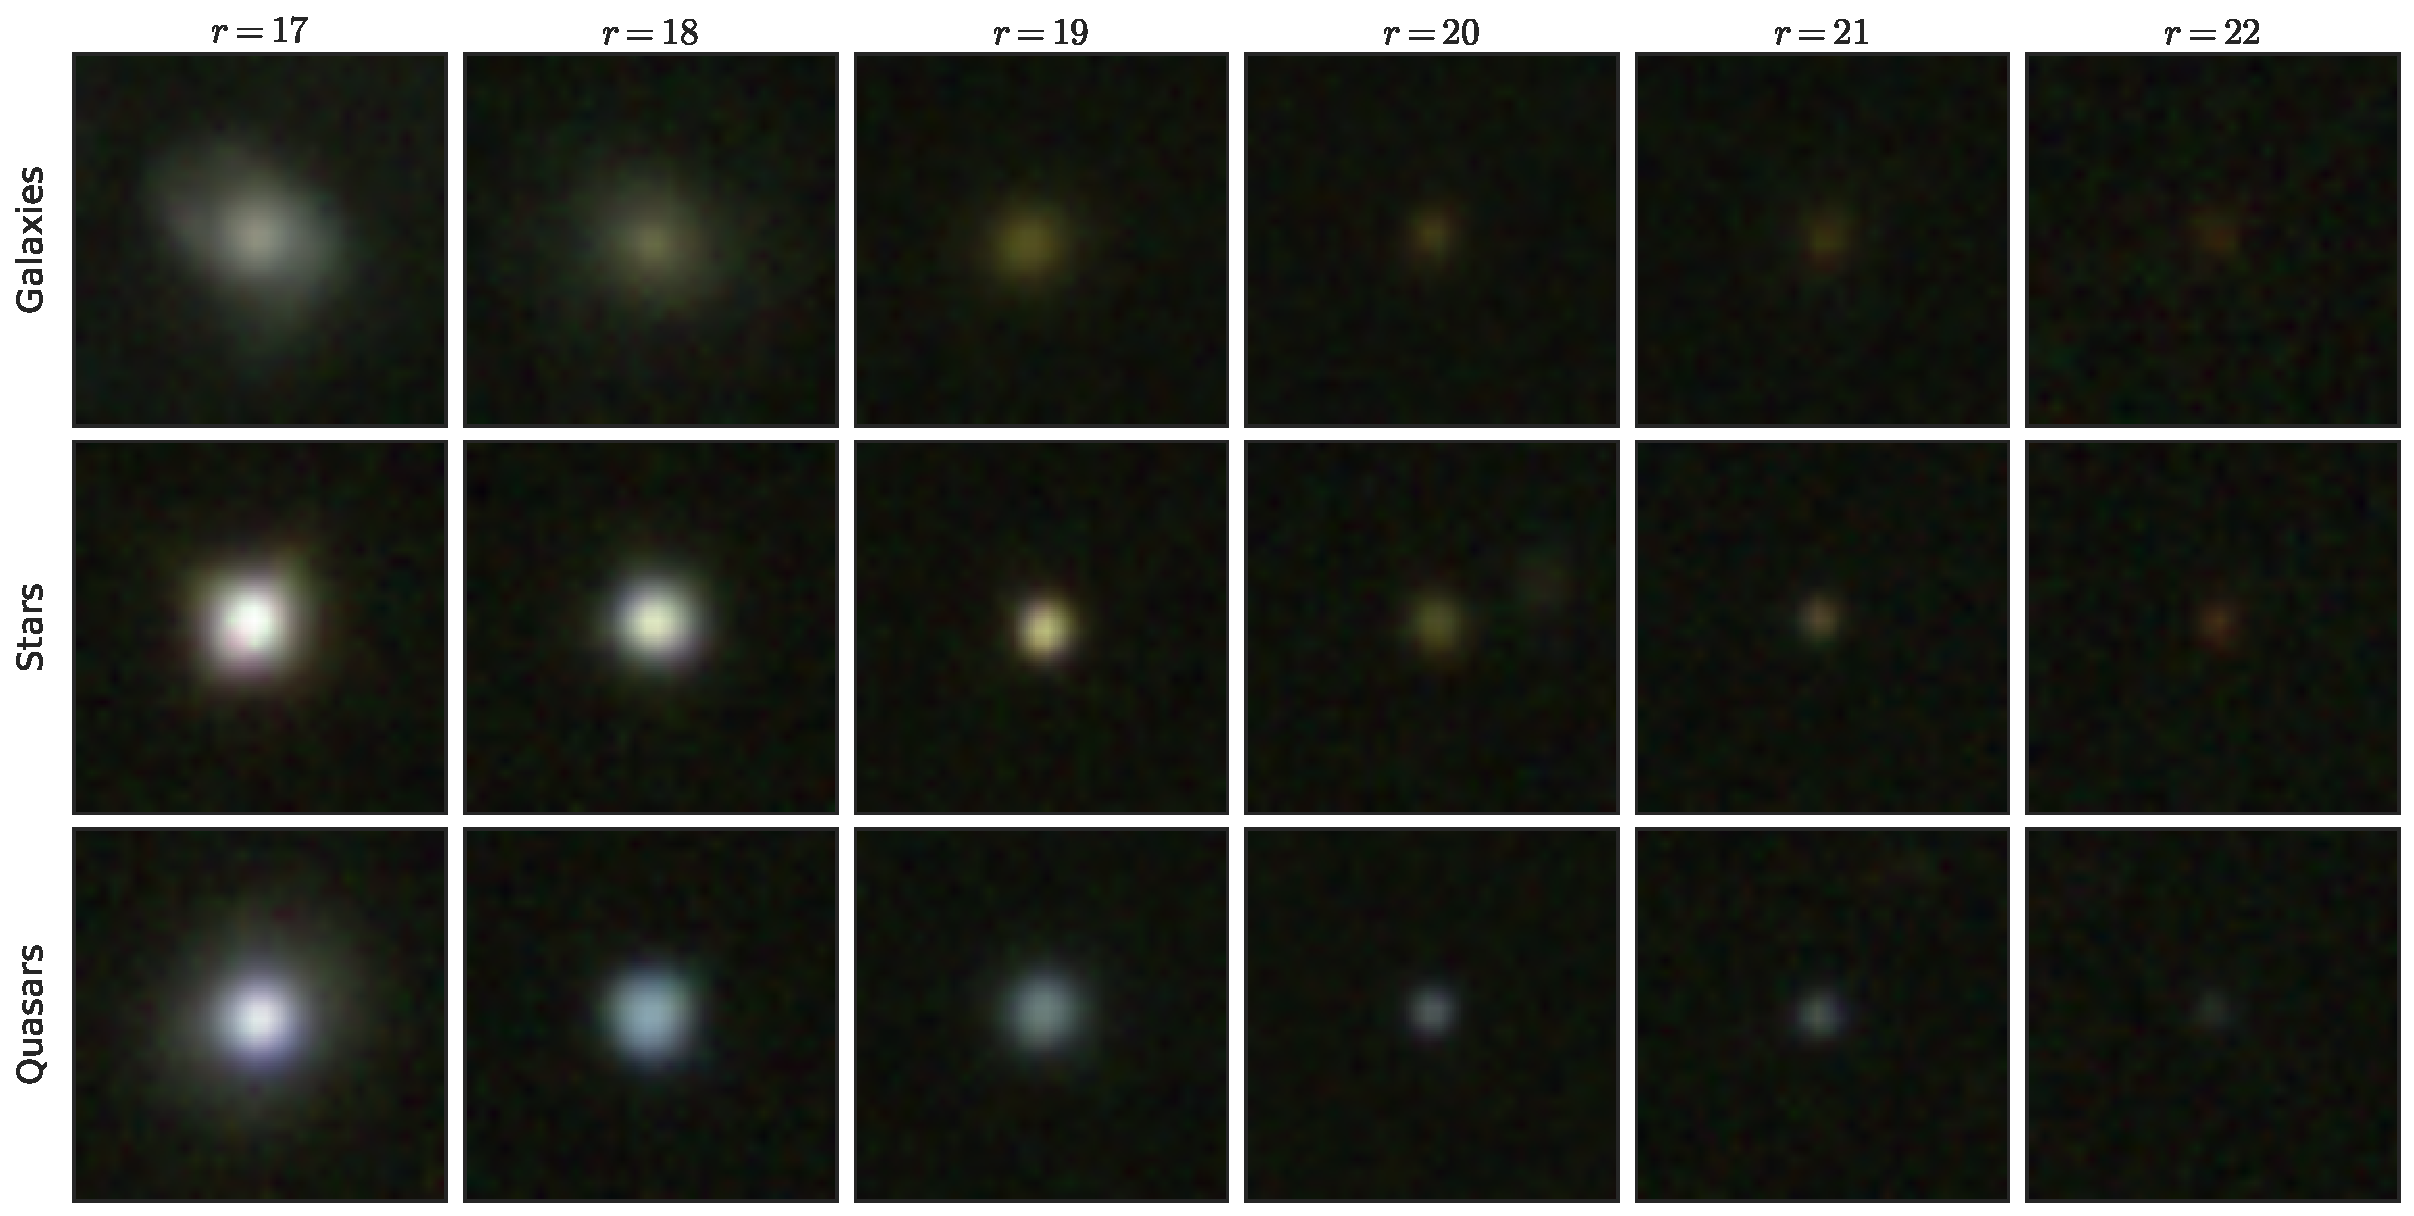
\includegraphics[width=\textwidth]{figures/sdss_stamps.pdf}
      \captionof{figure}{
        Postage stamp images showing typical stars, galaxies, and quasars in SDSS as a function of $r$-band magnitude.
        The magnitude corresponds to \texttt{SExtractor}'s \texttt{MAG\_AUTO} (Kron-like elliptical aperture magnitude).
        Each image is $32 \times 32$ pixels and centered on the source of interest.
        The RGB image is created by mapping the R channel values to the $i$ band magnitude, G channel to $r$ band, and B to $g$ band.
        Each image is individually normalized for visualization purposes.}
      \label{fig:sdss_stamps}
    \end{minipage}}
\end{center}

\begin{center}
  \rotatebox[origin=c]{90}{
    \begin{minipage}{0.9\textheight}
      \includegraphics[width=\linewidth]{figures/gan_stamps.pdf}
      \captionof{figure}{
        Sample $32 \times 32$ RGB images generated by our feature-matching GAN model as a function of $r$ band magnitude.
        Although the generated images for bright objects are slightly blurry and lack some details,
        the model generated, faint objects appear indistinguishable from real, faint objects.
        Since most objects are faint, the magnitude and half-light radius statistics of GAN generated images are in good agreement
        with the SDSS distribution as shown in Section \ref{sec:image_stats}.
      }
      \label{fig:gan_stamps}
    \end{minipage}}
\end{center}

\begin{figure}
  \centering
  \includegraphics[width=\columnwidth]{figures/spec_phot.pdf}
  \caption{
    Number counts of SDSS objects as a function of the $r$-band magnitude as estimated by kernel density estimation (KDE).
    The blue curve shows the KDE of $1 \times 10^6$ objects in the unlabeled training set,
    which are randomly selected from the \texttt{PhotoObj} view.
    The green curve is the KDE of $2 \times 10^5$ objects in the labeled test set,
    which are randomly selected from the \texttt{SpecObj} view.
    We use the SDSS \texttt{cModelMag}, the composite model magnitude resulting from the best-fitting linear combination
    of the best-fit exponential and de Vaucouleurs fits.
    All KDEs presented here and throughout this chapter use a Guassian kernel and Silverman's rule to determine
    the kernel bandwidth \citep{silverman1986density}.
  }
  \label{fig:spec_phot}
\end{figure}

%%%%%%%%%%%%%%%%%%%%

\begin{figure}
  \centering
  \includegraphics[width=\columnwidth]{figures/mag_kde.pdf}
  \caption{
      Comparison of $r$-band magnitude distributions between real images in the SDSS photometric sample
      and GAN generated images.
      The blue curve shows the KDE of $1 \times 10^5$ objects in the unlabeled training set.
      The red curve shows the KDE of $1 \times 10^5$ objects generated by GAN.
      We use the \texttt{SExtractor}'s \texttt{MAG\_AUTO} values as an approximate total magnitude for each objects.
      }
  \label{fig:mag_kde}
\end{figure}

\begin{figure}
  \centering
  \includegraphics[width=\columnwidth]{figures/mag_qq.pdf}
  \caption{Q-Q plot comparing the distributions of $r$-band magnitudes between real SDSS images and GAN generated images.}
  \label{fig:mag_qq}
\end{figure}

\begin{figure}
  \centering
  \includegraphics[width=\columnwidth]{figures/size_kde.pdf}
  \caption{Comparison of half-light radius distributions between real images in the SDSS photometric sample
  and GAN generated images.}
  \label{fig:size_kde}
\end{figure}

\begin{figure}
  \centering
  \includegraphics[width=\columnwidth]{figures/size_qq.pdf}
  \caption{Q-Q plot comparing the distributions of half-light radius between real SDSS images and GAN generated images.}
  \label{fig:size_qq}
\end{figure}

\begin{figure}
  \centering
  \includegraphics[width=\columnwidth]{figures/loss_vs_n.pdf}
  \caption{Cross-entropy as a function of the number of labeled examples in the training set.}
  \label{fig:loss_vs_n}
\end{figure}

\begin{figure}
  \centering
  \includegraphics[width=\columnwidth]{figures/calibration_curve.pdf}
  \caption{
    Calibrations curve for galaxies (red), stars(green), and quasars (blue).
    We compare the true fraction to the probabilistic output generated by the classifier for each type
    of objects.
    The dashed line displays the ideal relationship.
    The $1 \sigma$ error bars are computed following \citet{paterno2004calculating}.}
  \label{fig:calibration_curve}
\end{figure}

\begin{figure}
  \centering
  \includegraphics[width=\columnwidth]{figures/gal_comp_pur.pdf}
  \caption{
    Galaxy completeness and purity values as functions of the $r$-band magnitude.
    The upper panel shows the differential counts for true galaxies in the test set.
    The lower panel shows the galaxy completeness and purity for the integrated counts.
    We use the threshold value of 0.826 to obtain overall completeness of $96\%$.
    The $1 \sigma$ error bars are calculated with a Bayesian method in
    \citet{paterno2004calculating}.}
  \label{fig:gal_comp_pur}
\end{figure}

\begin{figure}
  \centering
  \includegraphics[width=\columnwidth]{figures/star_comp_pur.pdf}
  \caption{
    Similar to Figure \ref{fig:gal_comp_pur} but showing completeness for stars.
    We use the threshold value of 0.977 to obtain overall completeness of $25\%$.
    }
  \label{fig:star_comp_pur}
\end{figure}

\begin{figure}
  \centering
  \includegraphics[width=\columnwidth]{figures/qso_comp_pur.pdf}
  \caption{
    Similar to Figure \ref{fig:gal_comp_pur} but showing completeness and purity for quasars.
    We use the threshold value of 0.541 to maximize $\sqrt{ c_q^2 + p_q^2 }$.
    }
  \label{fig:qso_comp_pur}
\end{figure}

\begin{figure}
  \centering
  \includegraphics[width=\columnwidth]{figures/mcmc_loss.pdf}
  \caption{
    Cross-entropy for different numbers of averaged forward passes in dropout sampling.
    The solid blue line indicates mean cross-entropy of 10 experiments, and the error bars are 1 standard deviation.
    The red dotted line shows the cross-entropy with no dropout at testing time.
    }
  \label{fig:mcmc_loss}
\end{figure}

\begin{figure}
  \centering
  \includegraphics[width=\columnwidth]{figures/uncertainty_vs_mag.pdf}
  \caption{
    Model uncertainty as a function of $r$-band magnitude for 10,000 randomly selected objects in the test set.
    Model uncertainty is measured by the standard deviation of 100 forward passes in dropout sampling.
    The red dotted line indicates the magnitude at which the number count of the SDSS spectroscopic sample peaks.
    }
  \label{fig:uncertainty_vs_mag}
\end{figure}


\clearpage
\bibliographystyle{plainnat}
\bibliography{thesisbib}
\chapter{Conclusions}
  \label{chapter5}
 
\section{Summary and Conclusions}

In Chapter \ref{chapter2}, we have presented and analyzed a novel star-galaxy classification framework
for combining star-galaxy classifiers using the CFHTLenS data.
In particular, we use four independent classification techniques:
a morphological separation method;
TPC, a supervised machine learning technique
based on prediction trees and a random forest;
SOMc, an unsupervised machine learning approach
based on self-organizing maps and a random atlas;
and HB, a Hierarchical Bayesian template-fitting method
that we have modified and parallelized.
Using data from the CFHTLenS survey,
we have considered different scenarios:
when an excellent training set is available with spectroscopic labels from
DEEP2, SDSS, VIPERS, and VVDS, and
when the demographics of sources in a low-quality training set
do not match the demographics of objects in the test data set.
We demonstrate that the Bayesian Model Combination (BMC) technique improves
the overall performance over any individual classification method
in both cases.

The problem of star-galaxy classification is a rich area for future research. It is unclear
if sufficient training data will be available in future ground-based surveys. Furthermore, in
large sky surveys such as DES and LSST, photometric quality is not uniform across the
sky, and a purely morphological classifier alone will not be sufficient, especially at faint
magnitudes. Given the efficacy of our approach, classifier combination strategies are likely
the optimal approach for currently ongoing and forthcoming photometric surveys. Future
studies could apply the combination technique described in Chapter \ref{chapter2} to other surveys
such as the DES. Our approach can also be extended more broadly to classify objects that
are neither stars nor galaxies (e.g., quasars). Finally, future studies could explore the use
of multi-epoch data, which would be particularly useful for the next generation of synoptic
surveys.

In Chapter \ref{chapter3}, we have presented a convolutional neural network for classifying stars and
galaxies in the SDSS and CFHTLenS photometric images.
For the CFHTLenS data set, the network is able to provide a classification that
is as accurate as a random forest algorithm (TPC), while the probability estimates of
our ConvNet model appear to be better calibrated.
When the same network architecture is applied to the SDSS data set,
the network fails to outperform TPC,
but the probabilities are still slightly better calibrated.
The major advantage of ConvNets is that useful features are learned
automatically from images, while traditional machine learning
algorithms require feature engineering as a separate process
to produce accurate classifications.

Deep learning is a rapidly developing field, and recent developments include
improved network architectures.
Future work could explore more ConvNet variants, such as the
Inception Module~\citep{szegedy2015going} and Residual Network~\citep{he2015deep}.
To improve the predictive performance,
we have combined the predictions of different models across multiple
transformations of the input images (Section~\ref{sec:bmc}).
To further improve the performance, we could also train several networks
with different architectures and combine the models.
For example, the winning solution of \cite{dieleman2015rotation}
for the Galaxy Zoo challenge was based on a ConvNet model,
and it required averaging many sets of predictions from models with different
neural network architectures.
It is also likely that the performance will be improved
not only by training multiple network architectures,
but also by combining them with different star-galaxy classifiers.
ConvNets could be included as a different machine learning paradigm in the
classifier combination framework to produce further improvements in
predictive performance.

Our ConvNet model is a supervised algorithm, and one of the criticisms
of supervised techniques is their difficulty in extrapolating past the limits
of available spectroscopic training data.
Since it is difficult to assess the classification performance without a deeper
spectroscopic sample, we evaluated the performance using a test set
that is drawn from the same underlying distribution as the spectroscopic sample.
However, when our ConvNet model---trained on sources from a spectroscopic sample--- is
applied to a photometric sample---which is often fainter than our training set---the
performance of ConvNet will be less reliable.
Combining our ConvNet model with unsupervised methods (\eg a template fitting
method) in the aforementioned meta-classification framework will
help improve the efficacy of star-galaxy classification
beyond the limits of spectroscopic training data.

In Chapter \ref{chapter4}, we have presented a semi-supervised generative adversarial network for classifying stars, galaxies, and quasars in the SDSS photometric images.
We have demonstrated that the brightness and size distributions of images generated by our generative model
are in good agreement with those of the SDSS photometric images.
However, unlike most work on GANs, our focus was not solely on the generation of realistic images.
By using a small number of labeled images in conjunction with a large amount of unlabeled training data,
we have shown that our semi-supervised GAN is able to provide a classification that is comparable to the state-of-the-art
supervised methods.
we have also demonstrated the use of various scientific tools to validate our deep generative model.
In astronomy, we have powerful techniques for characterizing classifications, even in the absence of spectroscopic labels.
In contrast, most of the data sets used in the deep learning community are composed of natural images and text corpuses,
which lack such statistical techniques,
and direct comparison between different generative models is often difficult 
\citep{theis2016note}.
As a result, Astronomy has the potential to provide robust frameworks for evaluation and interpretation of generative models.

We used photometry and spectra from the SDSS.
While the SDSS provides a rich data set for deep learning,
it is limited to the optical and near-infrared wavelengths.
Future studies could explore combining multiple photometry sources by matching the SDSS objects to
photometric objects in other surveys, such as GALEX, WISE, or UKIDSS.
Future studies could also explore different strategies to improve the quality of generated images.
For example, although we used feature matching in this work to obtain a strong classifier,
if the goal is to improve the quality of generated images, an alternative technique
called minibatch discrimination will likely work better \citep{salimans2016improved,dai2017good}.
Finally, future studies could investigate the application of deep generative models in other settings,
such as unsupervised classification, object segmentation, and redshift estimation.

\clearpage
\bibliographystyle{plainnat}
\bibliography{thesisbib}

%\appendix*
%\include{Appendix.tex}

\backmatter

%\bibliographystyle{plainnat}
%\bibliography{thesisbib}

\end{document}
\endinput
%%
